%%
%% edengths.tex - LaTeX2e thesis driver
%%
%% Copyright (C) 1998 George Taylor
%% Copyright (C) 2013 Mathew Topper <damm_horse@yahoo.co.uk>
%%
%% This file is part of the University of Edinburgh, Department of
%% Engineering LaTeX2e thesis template.
%% 
%% The University of Edinburgh, Department of Engineering LaTeX2e thesis
%% template is free software: you can redistribute it and/or modify
%% it under the terms of the GNU General Public License as published by
%% the Free Software Foundation, either version 3 of the License, or
%% (at your option) any later version.
%% 
%% The University of Edinburgh, Department of Engineering LaTeX2e thesis
%% template is distributed in the hope that it will be useful,
%% but WITHOUT ANY WARRANTY; without even the implied warranty of
%% MERCHANTABILITY or FITNESS FOR A PARTICULAR PURPOSE.  See the
%% GNU General Public License for more details.
%% 
%% You should have received a copy of the GNU General Public License
%% along with the University of Edinburgh, Department of Engineering
%% LaTeX2e thesis template.  If not, see <http://www.gnu.org/licenses/>.
%%
%%
%%   ABOUT
%%
%% This is the driver file for a Latex2e template which corresponds to the
%% regulations regarding layout of a thesis submitted within the University
%% of Edinburgh school of Engineering. It is not `official', but conforms
%% as best as possible to the regulation as detailed at:
%%
%% http://www.ed.ac.uk/schools-departments/science-engineering/current-students/
%% research/submitting-thesis
%%
%% Please feel free to alter the template to your own liking, but note that
%% the template is made available under the GNU GPL and must be similarly
%% licenced should you wish to release your modified template.
%%
%%
%%   CREDITS
%%
%% This template is an amalgamtion of an existing Edinburgh University,
%% Electrical Engineering PhD Thesis class file (jthesis-v1.cls) authored by
%% George S Taylor which was released under the GNU GPL.
%% Code is included from the dmathesis class Written by M. Imran
%% for a thesis according to the university of Durham regulation, which was
%% released without copyright. It also contains ideas (possibly code) from the
%% Princeton thesis class file (PrincetonThesis.cls), authored by Mike Nolta.
%% Mathew Topper, Eoghan Maguire and Bill Edwards forsaw the need to maintain a
%% more recent latex implementation of the thesis regulations and thus, this
%% project was born. It is hoped that the template will be maintained by the
%% Edinburgh Engineering PhD community once released.
%%
%%
%%   RECORD OF REVISIONS
%%
%%     Date      Programmer         Description of change
%%     ====      ==========         =====================
%%   21/06/10    Mathew Topper      First Try.
%%
%%   22/06/10                       Removed pdf option in favour of
%%                                  ifpdf package.
%%
%%   23/06/10                       Can now include appendix files
%%                                  rather than input. Need to include
%%                                  the file appendix/edengapp.tex
%%
%%                                  Added includeonly command.
%%
%%   13/10/10                       Removed the input of packages.tex
%%                                  this is now dealt with in the class
%%                                  file.
%%
%%   20/10/10                       Added 'nobib' option to stop the
%%                                  bibliography being printed and now
%%                                  the frontmatter is also entered in 
%%                                  an include statement.
%%
%%   29/10/10                       Added 'hyper' option to use hyperref
%%                                  to add clickable links.
%%
%%   04/04/11                       Set a qualification command to set
%%                                  a custom qualification on the front
%%                                  page.
%%
%%                                  Added 'nomencl' option to use the
%%                                  nomencl package to build a nomenclature.
%%                                  You need to run ./makenomencl.sh to build
%%                                  the nomenclature in linux
%%
%%   19/04/13                       Added some commented ``part'' definitions
%%

%%%% LOAD DOCUMENT CLASS

\documentclass[11pt,twoside,nopardent,notitlepage,fancychap,hyper]{edengths}

%% Class options go in the square brackets above
%% i.e. \documentclass[options]{edengths}

%% Default report class options are:
%% (These are automatically included)
%%
%% a4paper
%% openright - Start chapters on righthand side pages
%% titlepage - Title should be on it's own page
%%


%% Standard available report class options are:
%%
%% 10pt
%% 11pt
%% 12pt
%% draft
%% final
%% fleqno
%% leqno
%% oneside
%% twoside

%% edengths class specific options:
%%
%% subsubnos - Enable numbering of subsubsections (note: these don't
%%             appear in the contents)
%% nosans    - Don't use the sans serif headers and captions
%% nopardent - Remove paragraph indent and add a line skip
%% msfonts   - Use MS fonts rather than latex default
%% fancychap - Use fancy chapter headings like jthesis
%% crest     - Use a crest on the front page
%% labels    - Print labels in spine margin.
%% nobib     - do not print the bibliography
%% hyper     - Use the hyperref package to put clickable links into 
%%             the document. Use \autoref{fig:example} now instead of,
%%             say, figure~\ref{fig:example}. Settings are in
%%             edengfmt.tex.
%% nomencl   - Use the nomencl package. Example of it's usage are in
%%             front/nomencl.tex. The Nomenclature is called from
%%             front/frontmatr.tex

%% ADDITIONAL FORMATTING can be done in 'edengfmt.tex' where the page
%% dimensions, header/footers, table of contents and the names of 
%% the bibliography and other formatting settings can be altered.
%% IN PARTICULAR THE LINE SPACING IS SET IN 'edengfmt.tex' AND
%% THE HYPERREF OPTIONS ARE SET HERE TOO. THIS SETS THE NAME OF
%% THE PDF, FOR EXAMPLE.

%% The class file should automatically detect pdflatex and provide
%% the right options.

%%%% LOAD USER DEFINED PACKAGES.

%% These are in ``packages.tex'' file and is automattically loaded
%% by the class file

%%%% LOAD USER DEFINED COMMANDS.

%%
%% defintns.tex - User defined commands for edengths.tex
%%
%% Copyright (C) 2012 Mathew Topper <damm_horse@yahoo.co.uk>
%%
%% This file is part of the University of Edinburgh, Department of
%% Engineering LaTeX2e thesis template.
%% 
%% The University of Edinburgh, Department of Engineering LaTeX2e thesis
%% template is free software: you can redistribute it and/or modify
%% it under the terms of the GNU General Public License as published by
%% the Free Software Foundation, either version 3 of the License, or
%% (at your option) any later version.
%% 
%% The University of Edinburgh, Department of Engineering LaTeX2e thesis
%% template is distributed in the hope that it will be useful,
%% but WITHOUT ANY WARRANTY; without even the implied warranty of
%% MERCHANTABILITY or FITNESS FOR A PARTICULAR PURPOSE.  See the
%% GNU General Public License for more details.
%% 
%% You should have received a copy of the GNU General Public License
%% along with the University of Edinburgh, Department of Engineering
%% LaTeX2e thesis template.  If not, see <http://www.gnu.org/licenses/>.
%%
%%
%%   ABOUT
%%
%% This file contains the user defined commands for a Latex2e template which
%% corresponds to the regulations regarding layout of a thesis submitted within
%% the University of Edinburgh School of Engineering. It is not `official',
%% but conforms as best as possible to the regulation as detailed at:
%%
%%   http://www.scieng.ed.ac.uk/Postgraduate/PhD/settingoutyourthesis.htm
%%
%% Please feel free to alter the template to your own liking, but note that
%% the template is made available under the GNU GPL and must be similarly
%% licenced should you wish to release your modified template.
%%
%%
%%   CREDITS
%%
%% This template is an amalgamtion of an existing Edinburgh University,
%% Electrical Engineering PhD Thesis class file (jthesis-v1.cls) authored by
%% George S Taylor which was released under the GNU GPL.
%% Code is included from the dmathesis class Written by M. Imran
%% for a thesis according to the university of Durham regulation, which was
%% released without copyright. It also contains ideas (possibly code) from the
%% Princeton thesis class file (PrincetonThesis.cls), authored by Mike Nolta.
%% Mathew Topper, Eoghan Maguire and Bill Edwards forsaw the need to maintain a
%% more recent latex implementation of the thesis regulations and thus, this
%% project was born. It is hoped that the template will be maintained by the
%% Edinburgh Engineering PhD community once released.

%%%%%%%%%%%%%%%%%%%%%%%%%%%%%%%%%%%%%%%%%%%%%%%%%%%%%%%%%%%%%%%%%%%%%%%%%%
%%%%%%%%%%             Define your commands here              %%%%%%%%%%%%
%%%%%%%%%%%%%%%%%%%%%%%%%%%%%%%%%%%%%%%%%%%%%%%%%%%%%%%%%%%%%%%%%%%%%%%%%%

%% New commands can be written using
%%    \newcommand{command}[inputs]{definition}.
%% In the definition the inputs are accessed with #1, #2, etc.
%%
%% If you want to override an existing command use \renewcommand instead
%% of \newcommand. \newcommand with give an error if command is already
%% defined.

%% If you are concerned that your command might override a default
%% you can use \providecommand which will ignore the new command if
%% a command of that name already exists.

%%%%% Some Example Maths Definitions (only use in maths mode)

\newcommand{\pdif}[2]{\frac{\partial #1}{\partial #2}}
%% ie \pdif{x}{t} would give partial x over t.

\newcommand{\dpdif}[2]{\dfrac{\partial #1}{\partial #2}}
%% inline partial derivative ie for $\dpdif{x}{t}$.
%% (\dfrac needs amsmath package)

\newcommand{\Ddif}[2]{\frac{D #1}{D #2}}
%% Material derivative

\newcommand{\spdif}[2]{\frac{\partial^{2} #1}{\partial #2^{2}}}
%% second partial derivative.

\newcommand{\altspdif}[3]{\frac{\partial^{2} #1}{\partial #2 \partial #3}} 
% mixed second partial i.e. \altspdif{x}{z}{t} = d2x / dzdt

\newcommand{\ndif}[2]{\frac{\mathrm{d} \, #1}{\mathrm{d} #2}}
%% ordinary differential.

\newcommand{\sndif}[2]{\frac{\mathrm{d} \,^{2} #1}{\mathrm{d} #2^{2}}}
%% ordinary second differential.


%%%% FOR NOMENCLATURE
\usepackage[intoc]{nomencl}
\makenomenclature

\usepackage{etoolbox}
\renewcommand\nomgroup[1]{%
	\item[\bfseries
		\ifstrequal{#1}{P}{Parameters}{%
		\ifstrequal{#1}{V}{Variables}{%
		\ifstrequal{#1}{D}{Decorations}{%
		\ifstrequal{#1}{S}{Subscripts}{%
		\ifstrequal{#1}{T}{Superscripts}{%
		\ifstrequal{#1}{N}{Distributions and Mathematical Foundations}{%
		\ifstrequal{#1}{A}{Abbreviations}{%
		\ifstrequal{#1}{U}{Units}{}}}}}}}}%
	]}

% This will add the units
%----------------------------------------------
\newcommand{\nomunit}[1]{%
	\renewcommand{\nomentryend}{\hspace*{\fill}#1}}
%----------------------------------------------

%\usepackage[toc]{glossaries}
%\makeglossaries
\usepackage{makeidx}
\makeindex

\usepackage{bm}
\usepackage{comment}
\usepackage{epstopdf}
\usepackage{graphicx}
\usepackage{xfrac}
\usepackage{algorithm}
%\usepackage[ruled, vlined, linesnumbered]{algorithm2e}
\usepackage{algpseudocode}
\usepackage{setspace}
\usepackage{lscape}
\usepackage{longtable}

\usepackage{tikz}
\def\checkmark{\tikz\fill[scale=0.4](0,.35) -- (.25,0) -- (1,.7) -- (.25,.15) -- cycle;}

%\usepackage[sorting=none]{bibtex}
\usepackage[compress]{cite}

\usepackage{pgfplots}
\usepackage{array}
\usepackage{colortbl}

\usepackage{adjustbox}
\newcolumntype{R}[2]{%
	>{\adjustbox{angle=#1,lap=\width-(#2)}\bgroup}%
	l%
	<{\egroup}%
}
\newcommand*\rot{\multicolumn{1}{R{90}{1em}}}% no optional argument here, please!

\algnewcommand\algorithmicforeach{\textbf{for each}}
\algdef{S}[FOR]{ForEach}[1]{\algorithmicforeach\ #1\ \algorithmicdo}

\def\cdf(#1)(#2)(#3){0.5*(1+(erf((#1-#2)/(#3*sqrt(2)))))}%
% to be used: \cdf(x)(mean)(variance)

\DeclareMathOperator{\CDF}{cdf}

%%%% SET THE PATH FOR DIAGRAMS.

\graphicspath{{chapter1/}{chapter2/}}%{chapter4/}
% {chapter_5/}{chapter_6/}{appendix/}}

%%%% PATH TO CREST

%% If you're not using the default crest files add the path here.
%% The default files are found in the 'front' directory.
%% Note: latex needs a eps file, while pdflatex needs pdf or jpg.
% \crestfile{/path/to/crest.pdps}

%%%% TITLE DETAILS

%% Author
\author{Fabian Neumann}

%% Title
\title{Optimal Scheduling of Electric Vehicles in Distribution Networks}

%% Qualification (Defaults to \textit{Doctor of Philosphy})
 \qualification{Master of Science}

%% University (Defaults to \textsc{The University of Edinburgh})
% \university{}

%% Year of submission
\date{August 2017}

%% NOTE - IF YOUR USING hyper THEN THE ABOVE DETAILS NEED SET IN
%% edengfmt.tex AS WELL.

%%%% CHAPTERS TO INCLUDE

%% You may restrict which chapters are compiled using \includeonly
%% appendix/edengapp must be in the list if appendicies are included.
%% To not print the bibliography use the nobib class option.

%% TURN ON nobib
% \includeonly{front/frontmtr, chapter1/chapter1}
% \includeonly{chapter2/chapter2, chapter3/chapter3}

%% TURN OFF nobib
% \includeonly{chapter6/chapter6, appendix/edengapp,
%              appendix/appendx1 appendix/appendix2}

\newlength\longest

% Math Definitions
\newcommand{\pev}{P^{EV}_{k,t}}
\newcommand{\pevi}{P^{EV}_{i,t}}
\newcommand{\pevc}{P^{EV}_{k,\tau}}
\newcommand{\pevb}{P^{EV}_{k,t-1}}
\newcommand{\aev}{\hat{\alpha}^{EV}_{k,t}}
\newcommand{\aevb}{\hat{\alpha}^{EV}_{k,t-1}}
\newcommand{\lev}{\omega_{k,t}}
\newcommand{\tabitem}{~~\llap{\textbullet}~~}


\renewcommand\floatpagefraction{.9}
\renewcommand\dblfloatpagefraction{.9} % for two column documents
\renewcommand\topfraction{.9}
\renewcommand\dbltopfraction{.9} % for two column documents
\renewcommand\bottomfraction{.9}
\renewcommand\textfraction{.1}   
\setcounter{totalnumber}{50}
\setcounter{topnumber}{50}
\setcounter{bottomnumber}{50}

\clubpenalty=9996
\widowpenalty=9999

%\expandafter\def\expandafter\normalsize\expandafter{%
%	\normalsize
%	\setlength\abovedisplayskip{-5pt}
%	\setlength\belowdisplayskip{5pt}
%	\setlength\abovedisplayshortskip{-5pt}
%	\setlength\belowdisplayshortskip{5pt}
%}

%%%% START DOCUMENT

\begin{document}

% some definitions
\pgfmathdeclarefunction{gauss}{2}{%
	\pgfmathparse{1/(#2*sqrt(2*pi))*exp(-((x-#1)^2)/(2*#2^2))}%
}

%%%% FRONT MATTER

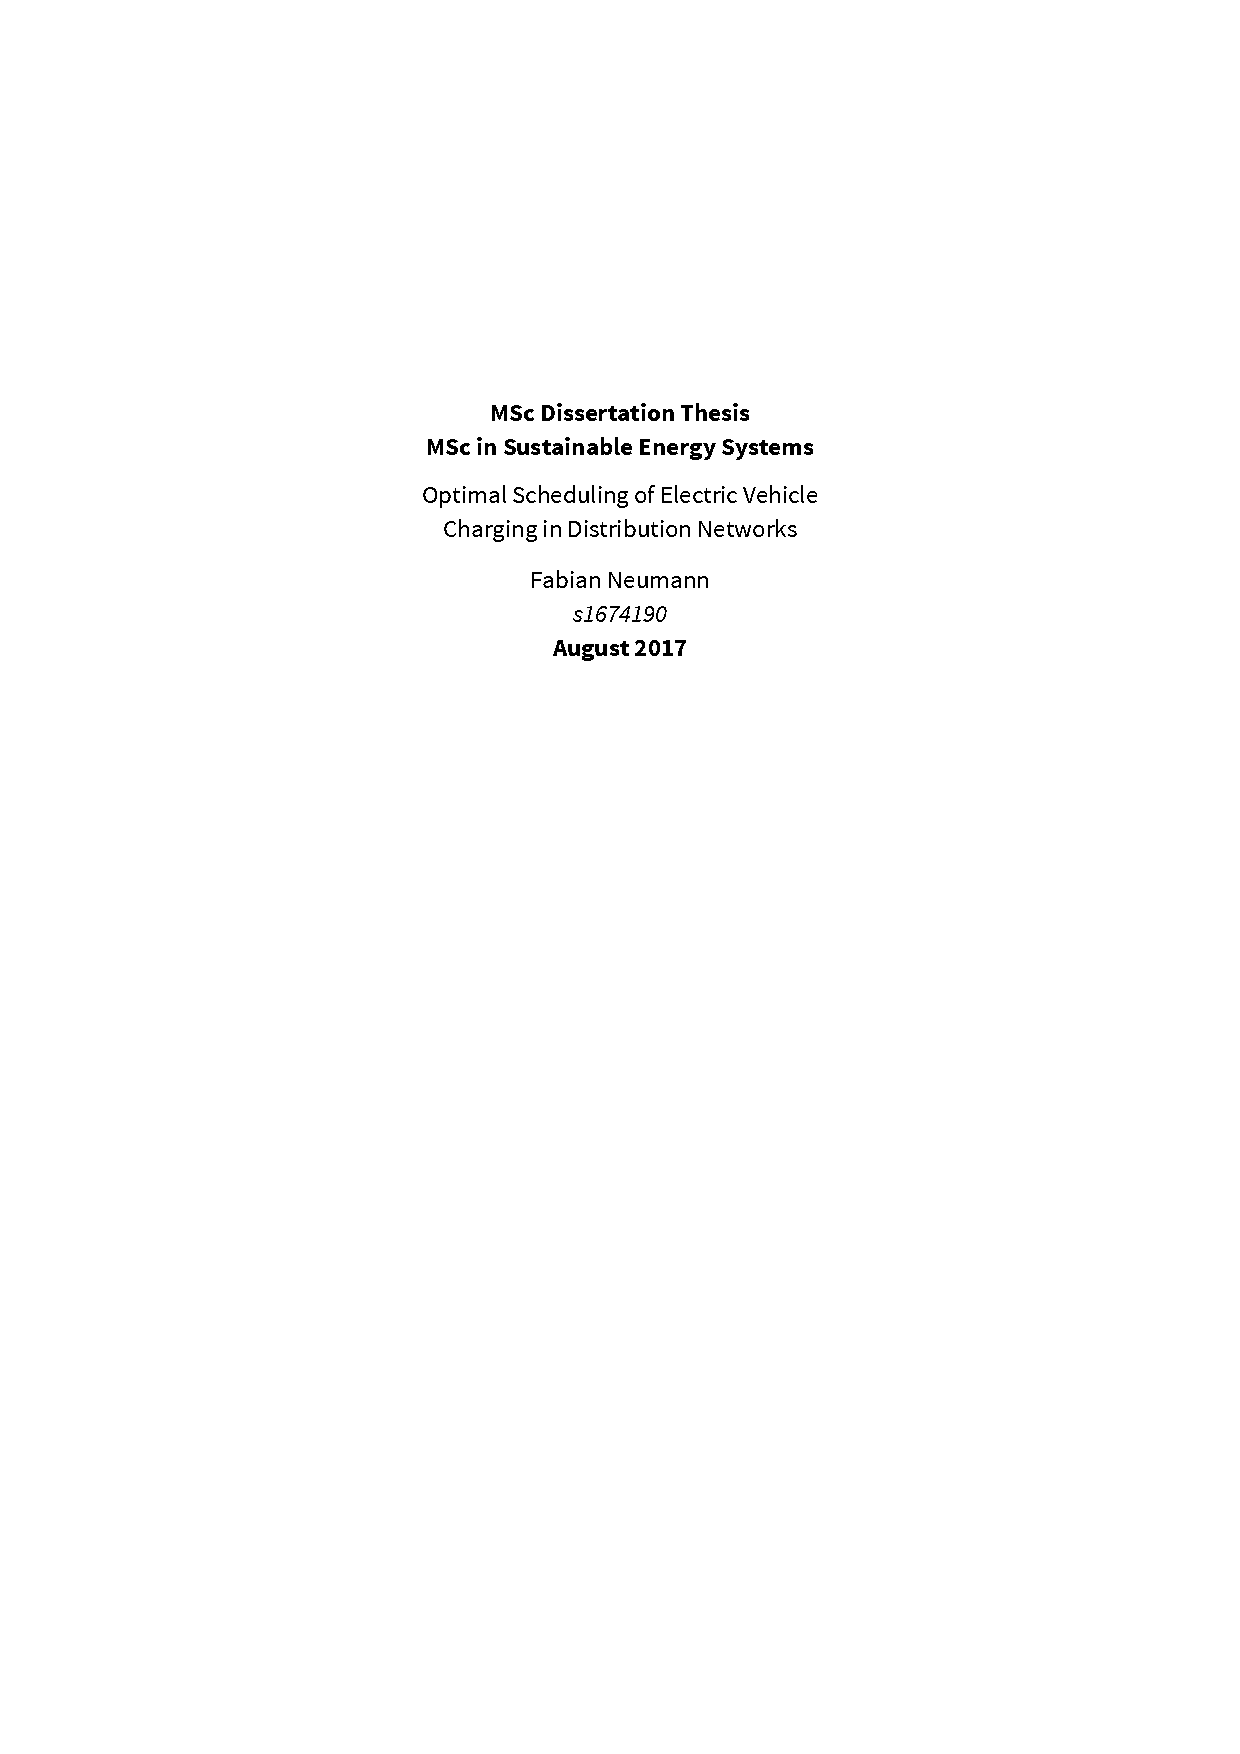
\includepdf{title}
\cleardoublepage

%%
%% frontmtr.tex - LaTeX2e thesis class
%%
%% Copyright (C) 2012 Mathew Topper <damm_horse@yahoo.co.uk>
%%
%% This file is part of the University of Edinburgh, Department of
%% Engineering LaTeX2e thesis template.
%% 
%% The University of Edinburgh, Department of Engineering LaTeX2e thesis
%% template is free software: you can redistribute it and/or modify
%% it under the terms of the GNU General Public License as published by
%% the Free Software Foundation, either version 3 of the License, or
%% (at your option) any later version.
%% 
%% The University of Edinburgh, Department of Engineering LaTeX2e thesis
%% template is distributed in the hope that it will be useful,
%% but WITHOUT ANY WARRANTY; without even the implied warranty of
%% MERCHANTABILITY or FITNESS FOR A PARTICULAR PURPOSE.  See the
%% GNU General Public License for more details.
%% 
%% You should have received a copy of the GNU General Public License
%% along with the University of Edinburgh, Department of Engineering
%% LaTeX2e thesis template.  If not, see <http://www.gnu.org/licenses/>.
%%
%%
%%   ABOUT
%%
%% This is the frontmatter file for a Latex2e template which corresponds to the
%% regulations regarding layout of a thesis submitted within the University
%% of Edinburgh School of Engineering. It is not `official', but conforms
%% as best as possible to the regulation as detailed at:
%%
%% http://www.ed.ac.uk/schools-departments/science-engineering/current-students/
%% research/submitting-thesis
%%
%% Please feel free to alter the template to your own liking, but note that
%% the template is made available under the GNU GPL and must be similarly
%% licenced should you wish to release your modified template.
%%
%%
%%   CREDITS
%%
%% This template is an amalgamtion of an existing Edinburgh University,
%% Electrical Engineering PhD Thesis class file (jthesis-v1.cls) authored by
%% George S Taylor which was released under the GNU GPL.
%% Code is included from the dmathesis class Written by M. Imran
%% for a thesis according to the university of Durham regulation, which was
%% released without copyright. It also contains ideas (possibly code) from the
%% Princeton thesis class file (PrincetonThesis.cls), authored by Mike Nolta.
%% Mathew Topper, Eoghan Maguire and Bill Edwards forsaw the need to maintain a
%% more recent latex implementation of the thesis regulations and thus, this
%% project was born. It is hoped that the template will be maintained by the
%% Edinburgh Engineering PhD community once released.
%%
%%
%%   RECORD OF REVISIONS
%%
%%     Date      Programmer        Description of change
%%     ====      ==========        =====================
%%   19/10/10    Mathew Topper     Ported from thesis.tex
%%                                 to allow the front matter
%%                                 to be included.
%%
%%   04/04/11                      Added some info about
%%                                 \frontchapter command.
%%
%%                                 Added \printglossary command
%%                                 to output nomenclature.
%%
%%

%% The special formatting in the class requires the use of
%% a particular command to call the front matter for everything
%% before the table of contents. Just supply the path to the
%% file containing the pre content front matter.

\makeprecontent{front/precntnt.tex}

%%%% TABLES AND LISTS

\phantomsection%
\addcontentsline{toc}{chapter}{Contents}%
\setstretch{1.4} 
%% Table of contents
\tableofcontents
\setstretch{1.45} 

%% Make the nomenclature. This command won't do anything if nomencl option
%% is not declared.

%\nomenclature[A, 02]{$c$}{Speed of light in a vacuum inertial system 
%	\nomunit{$299,792,458\, m/s$}}

\nomenclature[P]{$w_{max}$}{Maximum window size of demand peaks (hours)}
\nomenclature[P]{$w$}{Temporal shift of residential demand (hours)}
\nomenclature[P]{$T$}{Optimisation horizon in slots, transposition operator}
\nomenclature[P]{$K$}{Number of households}
\nomenclature[P]{$L$}{Number of transmission lines}
\nomenclature[P]{$\Delta t$}{Granularity, resolution, slot length (hours)} 
\nomenclature[P]{$D_{k,t}$}{Residential electricity demand of household $k$ in slot $t$ (kW)}
\nomenclature[P]{$\zeta$}{Consumption rate of electric vehicles (kWh/km)}
\nomenclature[P]{$B_{max}$}{Battery capacity of electric vehicles (kWh)}
\nomenclature[P]{$\eta$}{Charging efficiency} 
\nomenclature[P]{$P^{EV}_{max}$}{Maximum EV charging rate (kW)}
\nomenclature[P]{$P^{EV}_{min}$}{Minimum EV charging rate (kW)}
\nomenclature[P]{$\Delta^{EV}_{max}$}{Maximum rate of change of charging power (kW)}
\nomenclature[P]{$\delta_{mil}$}{Daily mileage of an electric vehicle (miles)}
\nomenclature[P]{$\tau_{arr}$}{Arrival time of an electric vehicle (minutes)}
\nomenclature[P]{$\tau_{dep}$}{Departure time of an electric vehicle (minutes)}
\nomenclature[P]{$\tau_{init}$}{Time of the day in minutes at which the optimisation routine starts (minutes)}
\nomenclature[P]{$\mu_{mil}$}{Average daily mileage (miles)}
\nomenclature[P]{$\mu_{arr}$}{Average arrival time (minutes)}
\nomenclature[P]{$\mu_{dep}$}{Average departure time (minutes)}
\nomenclature[P]{$\sigma_{mil}$}{Standard deviation of daily milage (miles)}
\nomenclature[P]{$\sigma_{arr}$}{Standard deviation of arrival times (minutes)}
\nomenclature[P]{$\sigma_{dep}$}{Standard deviation of departure times (minutes)}
\nomenclature[P]{$B^{arr}_{k}$}{Initial battery charge level of electric vehicle at household $k$ (kWh)}
\nomenclature[P]{$\alpha^{EV}_{k,t}$}{Vehicle availability at slot $t$ at household $k$} 
\nomenclature[P]{$\bar{\pi}$}{Average spot price (p/kWh)} 
\nomenclature[P]{$\pi$}{Input price profile (p/kWh)} 
\nomenclature[P]{$\pi'$}{Temporally extended price input profile (p/kWh)} 
\nomenclature[P]{$\pi^{EPEX}_t$}{Pure spot market price at time slot $t$ (p/kWh)} 
\nomenclature[P]{$q$}{Static price surcharge (p/kWh)} 
\nomenclature[P]{$s$}{Price spreading factor} 
\nomenclature[P]{$\xi$}{Sequence of red Gaussian noise where $\xi_t \sim \mathcal{N}(0,1)$}
\nomenclature[P]{$\kappa$}{Sequence of factors describing the severity of price uncertainty}
\nomenclature[P]{$\omega$}{Sequence of white Gaussian noise}
\nomenclature[P]{$\rho$}{Regulation service price (p/kW$\cdot$h)}
\nomenclature[P]{$\bm{\mu}$}{Network voltage sensitivity matrix (V/kW)}
\nomenclature[P]{$\bm{\lambda}$}{Network line loading sensitivity matrix (A/kW)}
\nomenclature[P]{$C$}{Objective function of problem (p)}
\nomenclature[P]{$C'$}{Objective function of problem including regulation service provision (p)}
\nomenclature[P]{$\gamma_{min}$}{Battery charge level threshold for the provision of regulation service}
\nomenclature[P]{$V_{k,t}^{bus}$}{Terminal phase voltage (V)}
\nomenclature[P]{$V_{k,t,init}^{bus}$}{Initial terminal phase voltage without electric vehicles (V)}
\nomenclature[P]{$V_{min}$}{Minimum phase voltage (V)}
\nomenclature[P]{$V_{max}$}{Maximum phase voltage (V)}
\nomenclature[P]{$I^{line}_{\ell,t}$}{Current through cable $\ell$ in slot $t$ (A)}
\nomenclature[P]{$I^{max}_{\ell}$}{Rated ampacity of cable $\ell$ (A)}
\nomenclature[P]{$S_t^{tr}$}{Apparent power flowing through the transformer (kVA)}
\nomenclature[P]{$S_{max}^{tr}$}{Maximum allowed apparent power flowing through the transformer (kVA)}
\nomenclature[P]{$\sigma$}{Indices of sorted prices in ascending order}
\nomenclature[P]{$\theta$}{Priority list (order in which electric vehicles are scheduled)}
\nomenclature[P]{$D_k^{EV}$}{Electric vehicle energy demand (kWh)}
\nomenclature[P]{$T_{viol}$}{Subset of slots $T$ with technical constraint violations}
\nomenclature[P]{$\Delta P$}{Incremental step size of load limitation (kW)}
\nomenclature[P]{$\nu_{\alpha}$}{Degree of certainty that vehicle is available}
\nomenclature[P]{$\nu_{B}$}{Degree of certainty that initial battery charge level is no less than entered}
\nomenclature[P]{$\nu_{\pi}$}{Degree of certainty that price is not higher}

% distributions
\nomenclature[N]{$\mathcal{U}(a,b)$}{Uniform distribution on the interval $[a,b]$}
\nomenclature[N]{$\mathcal{N}(\mu,\sigma)$}{Univariate normal distribution with mean $\mu$ and standard deviation $\sigma$}
\nomenclature[N]{$\mu$}{Mean, location parameter of logistic distribution}
\nomenclature[N]{$\sigma$}{Standard deviation}
\nomenclature[N]{$\Gamma(x)$}{Gamma function}
\nomenclature[N]{$f$}{Probability distribution function}
\nomenclature[N]{$F$}{Cumulative distribution function}
\nomenclature[N]{$a$}{Shape parameter of Gamma distribution}
\nomenclature[N]{$\theta$}{Scale parameter of Gamma distribution}
\nomenclature[N]{$\displaystyle e$}{Euler's number}
\nomenclature[N]{$s$}{Scale parameter of logistic distribution}
\nomenclature[N]{$\sigma^2$}{Variance}
\nomenclature[N]{$\gamma_1$}{Skewness of a distribution}
\nomenclature[N]{$\gamma_2$}{Kurtosis of a distribution}
\nomenclature[N]{$\lambda$}{Rate parameter of the exponential distribution}
\nomenclature[N]{$F^{-1}$}{Inverse cumulative distribution function}
\nomenclature[N]{$F^{-1}$}{Inverse cumulative distribution function}
\nomenclature[N]{$\mathcal{N}_i(\bm{\mu},\bm{\rho})$}{Multivariate normal distribution with means $\bm{\mu}\in \mathbb{R}^i$ and matrix of correlation coefficients $\bm{\rho}\in \mathbb{R}^{i\times i}$}
\nomenclature[N]{$Z$}{Bivariate random variable}
\nomenclature[N]{$X$}{Bivariate random variable}
\nomenclature[N]{$W$}{Univariate random variable}
\nomenclature[N]{$w$}{Realisation of random variable $W$}
\nomenclature[N]{$x_i$}{i-th realisation of random variable $X$}
\nomenclature[N]{$z_i$}{i-th realisation of random variable $Z$}
\nomenclature[N]{$r$}{Sample Pearson correlation coefficient, lag-1 autocorrelation}
\nomenclature[N]{$\mathcal{M}$}{Generic multivariate distribution}
\nomenclature[N]{$\mathcal{M}_i$}{Marginal distribution of generic multivariate distribution}
\nomenclature[N]{$\mathbb{E}[X]$}{Expectation value of a random variable $X$}
\nomenclature[N]{$\mathbb{P}(x=X)$}{Probability of $x$ being realised from a random variable $X$}
\nomenclature[N]{$\Phi$}{Cumulative distribution function of standard normal distribution $\mathcal{N}(0,1)$}
\nomenclature[N]{$\mathbb{B}$}{Set of binary numbers}
\nomenclature[N]{$\mathbb{R}$}{Set of real numbers}
\nomenclature[N]{$\mathbb{N}$}{Set of natural numbers}
\nomenclature[N]{$\bm{0}_{X,Y}$}{Zero matrix with dimensions $X\times Y$}
\nomenclature[N]{$\bm{\rho}$}{Matrix of correlation coefficients}

%subscripts
\nomenclature[S]{$k$}{Node with household connected}
\nomenclature[S]{$t$}{Time slot}
\nomenclature[S]{$\ell$}{Line identifier}

%variables
\nomenclature[V]{$P^{EV}_{k,t}$}{Charging rate of electric vehicel at household $k$ in time slot $t$ (kW)}
\nomenclature[V]{$\omega_{k,t}$}{Regulation service provision of EV at household $k$ in time slot $t$}

%decorations
\nomenclature[D]{$\tilde{}$}{Uncertain parameter}
\nomenclature[D]{$\hat{}$}{Estimate for uncertain parameter}
\nomenclature[D]{$\bar{}$}{Average value}

%glossary
\nomenclature[A]{AC}{Alternating Current}
\nomenclature[A]{EV}{Electric vehicle}
\nomenclature[A]{EPEX}{European Power Exchange}
\nomenclature[A]{UKPX}{United Kingdom Power Exchange}
\nomenclature[A]{SOC}{State of charge}
\nomenclature[A]{EU}{European Union}
\nomenclature[A]{USA, US}{United States of America}
\nomenclature[A]{MPC}{Model Predictive Control}
\nomenclature[A]{DG}{Distributed generation}
\nomenclature[A]{DSM}{Demand side management}
\nomenclature[A]{DR}{Demand response}
\nomenclature[A]{TSO}{Transmission system operator}
\nomenclature[A]{DSO, DNO}{Distribution system/network operator}
\nomenclature[A]{ICT}{Information and communication technology}
\nomenclature[A]{ADMM}{Alternating Direction Method of Multipliers}
\nomenclature[A]{UK}{United Kingdom}
\nomenclature[A]{PV}{Photovoltaic}
\nomenclature[A]{V2G}{Vehicle-to-Grid}
\nomenclature[A]{CHP}{Combined heat and power}
\nomenclature[A]{ANM}{Active Network Management}
\nomenclature[A]{PF}{Power Flow}
\nomenclature[A]{ULEV}{Ultra low emission vehicles}
\nomenclature[A]{DC}{Direct Current}
\nomenclature[A]{IEC}{International Electrotechnical Commission}
\nomenclature[A]{ISO}{International Organization for Standardization}
\nomenclature[A]{CO$_2$}{Carbon dioxide}
\nomenclature[A]{PDF}{Probability Distribution Function}
\nomenclature[A]{CDF}{Cumulative Distribution Function}
\nomenclature[A]{RPD}{Reference Price Data}
\nomenclature[A]{APX}{Amsterdam Power Exchange}
\nomenclature[A]{OLTC}{On Load Tap Changer}
\nomenclature[A]{MC}{Monte Carlo}
\nomenclature[A]{MDP}{Markov Decision Process}
\nomenclature[A]{THD}{Total Harmonic Distortion}
\nomenclature[A]{IEEE}{Institute of Electrical and Electronics Engineers}
\nomenclature[A]{LV}{Low Voltage}
\nomenclature[A]{MV}{Medium Voltage}
\nomenclature[A]{OpenDSS}{Open-source electrical power Distribution System Simulator}
\nomenclature[A]{MATLAB}{Programming Language}
\nomenclature[A]{Python}{Programming Language}
\nomenclature[A]{Scipy}{Python library for scientific computing}
\nomenclature[A]{ELEXON}{Electric utility company in London}
\nomenclature[A]{LP}{Linear Programming, Linear Programme}
\nomenclature[A]{RTP}{Real time prices (type of electricity tariffs)}
\nomenclature[U]{kWh}{Kilowatt-hour (unit of energy)}
\nomenclature[U]{kW}{Kilowatt (unit of active power)}
\nomenclature[U]{kVA}{Kilovolt-amperes (unit of apparent power)}
\nomenclature[U]{kvar}{Kilovolt-amperes reactive (unit of reactive power)}
\nomenclature[U]{V}{Volt (unit of voltage)}
\nomenclature[U]{A}{Ampere (unit of current)}
\nomenclature[U]{h}{Hours (unit of time)}
\nomenclature[U]{min}{Minutes (unit of time)}
\nomenclature[U]{\pounds}{British Pound (unit of currency)}
\nomenclature[U]{p}{British Pence (sub-unit of currency: \pounds 1 = 100 p)}


% TODO check units
\printnomenclature[2.5cm]
\cleardoublepage

%\newglossaryentry{computer}
%{%
%	name=computer,
%	description={is a programmable machine that receives input,
%		stores and manipulates data, and provides
%		output in a useful format}
%}

%\printglossaries


%% Custom front matter chapters can be added using \input{frontchapter.tex}
%% For the correct title behaviour use the \frontchapter{title} command instead
%% of \chapter{title} at the start.


%% QUOTE
%{\clearpage
%	
%	\thispagestyle{empty}
%	\null\vfill
%	
%	\settowidth\longest{\large\itshape Beginning at the beginning, the King said, very gravely}
%	\centering
%	\parbox{\longest}{%
%		\raggedright{\large\itshape%
%			``Begin at the beginning,'' the King said, very gravely, \\
%			``and go on till you come to the end: then stop.'' \par\bigskip
%		}   
%		\raggedleft\MakeUppercase{Lewis Carroll, Alice in Wonderland}\par%
%	}
%	
%	\vfill\vfill
%	
%\clearpage}

%%%% START MAIN BODY TEXT

%% Call the edengths wrapper.
\startbody

%% Input the nomencl example if package is loaded.
\ifthenelse{\boolean{nomenclflag}}{
  \chapter{Nomencl Test}

\section*{Main equations}
\begin{equation}
  a=\frac{N}{A}
\end{equation}%
\nomenclature{$a$}{The number of angels per unit area}%
\nomenclature{$N$}{The number of angels per needle point}%
\nomenclature{$A$}{The area of the needle point}%
The equation $\sigma = m a$%
\nomenclature{$\sigma$}{The total mass of angels per unit area}%
\nomenclature{$m$}{The mass of one angel}
follows easily.

}{}

%\chapter{Test}
%
%Mein Test zur Nomenklatur
%
%\nomenclature{$m$}{mass}
%\printnomenclature

%% The template will work with part definitions (starred or otherwise), but note
%% that nameref and autoref may not work properly for referencing them.
% \part{The Fellowship of the Thing}


\chapter{Introduction}
\label{sec:intro}

\section{Motivation and Problem Statement}

\subsection{Political Targets and Market Uptake of Electric Vehicles}

The transport sector accounts for a significant proportion of the UK total energy consumption and is to date mainly based on fossil fuels (\Autoref{fig:energy}). Across the EU personal and freight road transport cause 23\% of carbon emissions in equal shares \cite{Eurostat2017}. The steady rise in greenhouse gases, as well as dwindling reserves, are driving the link between the transport sector and an electricity sector that will be increasingly powered by renewable energy sources. Against the backdrop of climate change, the UK government has defined ambitious aspirations for decarbonising mobility and electricity supply following the EU's 2009 Renewable Energy Directive. By 2020, the UK aims to source 15\% of all energy and 10\% of transport fuels from renewables \cite{ECCC2016}. To date, however, only 4.23\% of transport fuels are supplied by sustainable energy including biofuels, whereas the electricity sub-target of 30\% by 2020 is projected to be surpassed by an additional 4\% \cite{ECCC2016}.

\begin{figure}[]
	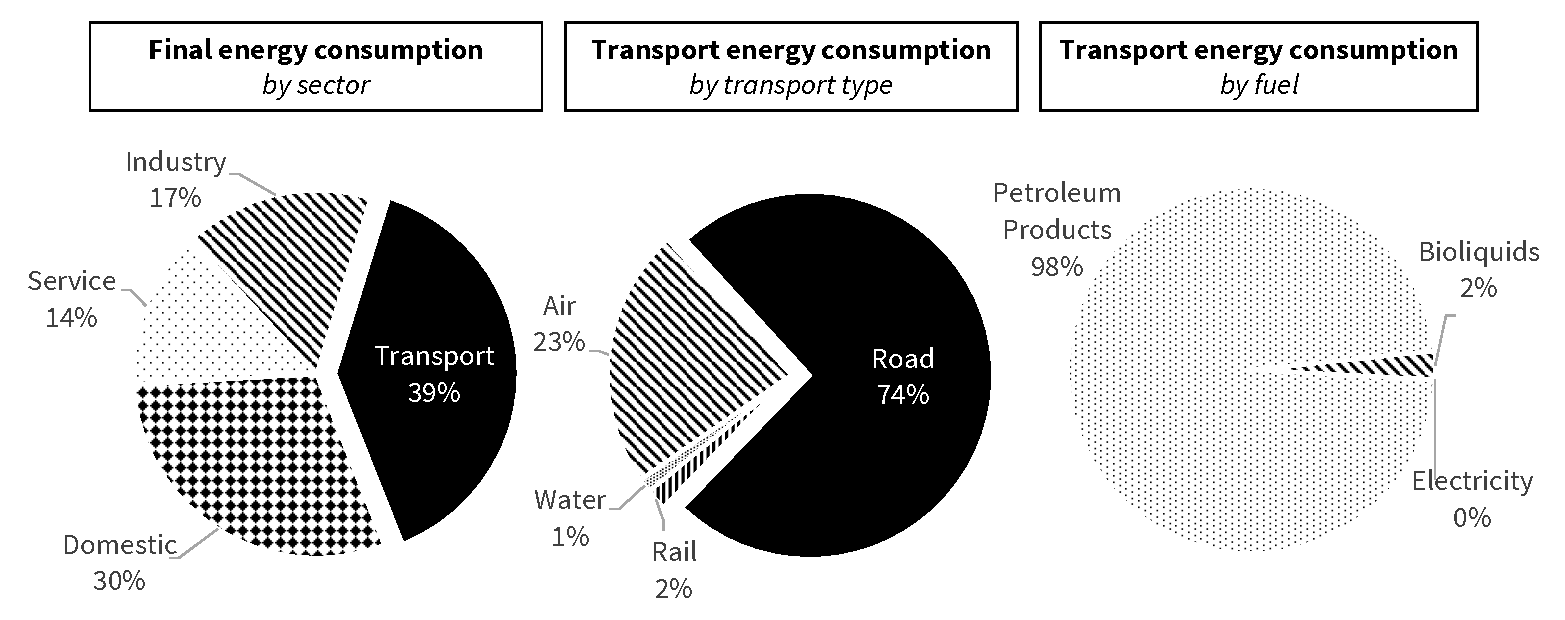
\includegraphics[width=\textwidth,trim={0cm 0cm 0cm 0cm},clip]{figures/energy.pdf}
	\caption{Final energy consumption of the UK by sector and fuel type for the year 2015 \cite{dfbei2017}}
	\label{fig:energy}
\end{figure}

The electrification of personal mobility is, nonetheless, a cornerstone of the UK's policy to reduce carbon emissions as well as air pollution in urban areas and is actively supported by government grant schemes and further incentives, which have overall been received favourably \cite{Knight2015}. The Plug-In Car Grant Scheme, operational since 2011, contributes a grant of 25\% but no more than \pounds 4,500 to the purchase cost of an eligible electric vehicle (EV). To date, more than 100,000 participants have made use of this incentive \cite{SMMT2017}. In 2013, the scheme was complemented with the Electric Vehicle Homecharge Scheme which reimburses costs for installing domestic charge points at home up to 75\%. Regional incentives such as the exemption from the London congestion charge add to the appeal of e-mobility.

Today, there are 87,000 electric vehicles on UK roads with new registrations peaking month to month \cite{ECCC2016}. While the market uptake is competitive compared to fellow European countries, electric vehicles yet only account for a marginal share of new car sales of approximately 2\% as of July 2017 \cite{SMMT2017}. However, recent news has nourished hope for progress. The car manufacturer Volvo pledged to exclusively produce electric vehicles from 2019 onwards \cite{Vaughan2017}. Tesla released its first long-range electric car Model 3 for the mass market, which has been praised for its affordability and excellent safety design \cite{Hern2017}. Most strikingly, in late July 2017 the UK government announced plans to ban all new petrol and diesel cars by 2040 in line with its previously published aspirations to have every new car powered by electricity by 2040 \cite{Knight2015}. By joining the Zero Emission Vehicle Alliance, the UK committed to a 100\% penetration rate of ultra low-emission vehicles (ULEV) in personal transport by 2050 \cite{ZeroEmissionVehicleAlliance2015}. Already for 2030, study \cite{Dof2008} predicts up to 20.6 million vehicles on UK roads in an extreme range scenario and at least 3 million under business as usual conditions.

\subsection{Challenges for Sustainable Electric Mobility}

% conditions
While the political will is a prerequisite, further conditions apply to achieve a sustainable transport sector. It must be untangled whether the transmission and distribution network capacity suffices to accommodate EV loads and how required supplemental renewable power can be integrated?

The additional load and rapid emergence of uncontrolled residential EV charging will negatively impact the low-voltage distribution network. The grid will be faced with an unprecedented energy demand, which had previously been supplied by diesel and petrol for ages. An average \mbox{3-person} household in the UK consumes \mbox{3,900 kWh} annually. With a consumption of \mbox{3,600 kWh}, an average EV with an annual mileage of \mbox{18,000 km} almost doubles overall electricity demand \cite{Knight2015}. Effects include excessive voltage drops, phase imbalances and overloading of network components, especially when many EVs charge simultaneously. Unfortunately, EV loads are likely to cluster when commuters arrive home at the end of the workday at similar times and plug-in their electric vehicles. Thus, immediate charging, especially in the evening at times of highest residual load, increases the detrimental impact. 

%% decarbonisation / renewable energy
Furthermore, a decarbonisation of electricity generation must accompany the expansion of electric vehicles since the specific CO$_2$-emissions of EVs depend largely on the composition of the generators that supply power at the time of charging current. Electric vehicles will only reveal their environmental supremacy over conventional vehicles if they are charged by renewable energy \cite{DLR2012}. Consequently, increased intermittent renewable energy generation will add to the need for smart grid management. Wind and photovoltaic power will take on an increasing share of electricity generation and are unable to follow electricity demand. Accordingly, there will be times when electricity demand is fully covered by renewable energy sources, but also those in which fossil fuels continue to dominate. For a safe power grid operation, demand and supply have to coincide exactly. Today it can be commonly observed that primarily wind turbines but also photovoltaic (PV) systems are shut down deliberately in order not to imperil grid stability in times of excess supply. For instance, the volume of unused energy by feed-in management trebled in 2014 compared to 2013 levels to 1.581 GWh in Germany as controllability on the supply side diminishes \cite{GermanysFederalNetworkAgency2016}.

\subsection{Solution Approaches for Sustainable Electric Mobility}

% Load flexibility / potential
Both aspects mandate increased levels of controllability on the demand side to reduce peak demand or match power supply; residential electricity demand becomes elastic. While investment in major network reinforcement is an intuitive measure to incorporate additional loads, it is deemed more economically efficient to encourage EV users to charge at off-peak times. Consensus exists that existing distribution networks can accommodate substantial penetration levels of electric vehicles if charging is coordinated. Exploiting typical load flexibility of parked electric vehicles by controlled charge scheduling as means of demand-side management will allow a mitigation of the network strains they evoke and can even provide a benefit to the grid integration of renewables \cite{Strbac2008}. This can be achieved by simple charge rate modulation with unidirectional power flow alone or additionally the provision of ancillary services with bidirectional power flow. Demand is fit to the current power supply by shifting loads under the umbrella of the renowned \textit{smart grid}, which \cite{Schuller2013} defines as the ``\textit{combination of enabling ICT \footnote{ICT = Information and Communication Technology} technologies that jointly make the power delivery infrastructure more reliable, versatile, secure and more accommodating for the integration of distributed and intermittent resources}''. Thereby, the electric vehicle unites aspects of an energy consumer and a regulation service provider simultaneously.

Traditionally, the network operators exercise balancing control using active and reactive power reserves offered by conventional generators and their costs are identified as intermittency costs of renewable energy generation, but under target-compliant market conditions controlled EV loads may intercept part of the demand and increase the resilience of power networks. Besides their load flexibility, electric vehicles are particularly suitable for demand side management for they can quickly respond to grid demand variation without startup or shutdown cost \cite{Han2011}. Moreover, EVs are already equipped with charge controllers and may implement profitable charging strategies \cite{Richardson2012}. \cite{Gottwalt2016} attests electric vehicles alongside stationary batteries and heat storages the most promising benefits for demand response.


%----------------------------
% Demand Side Management / Smart Grid / DR
%Definition of demand side management
%* all intentional electricity consumption pattern modifications by end-use customers, that are intended to alter the timing, level of instantaneous demand, or total electricity consumption
%Demand response (DR) can be defined as the changes in electricity usage by end-use customers from their normal consumption patterns in response to changes int he price of electricity over time or to incentive payments designded to induce lower electricity use at times of high wholesale market prices or when systems reliability is jeopardised (DoE2006, Albadi2008)
%Demand-Side Management (DSM) has traditionally been developed and centrally coordinated by utilities, often at the request of regulatory bodies seeking to minimize the operating cost base used to determine regulated tariffs for end users (Cooke2011)
% Dsm refers to classical, utility controlled meausres, while DR is the product of voluntary and independent decentralized decision-making by suppliers and customers.
%advantages \cite{Strbac2008}
%- reduction of generation reserves
%- capacity factor increase for available resources
%- reduction of emissions for power generation and balancing
%- improvement of transmission network efficiency
%- improvement of distribution network efficiency
%- improve the balancing of intermittent renewable energy sources
%- demand side elasticity in the power market
%Characteristics:
%- Low voltage grid
%- ICT to link and control devices
%- Decentral generation
%- Demand flexibility
%New Features:
%- Reliability: Due to using of Technologies for Fault-Detection
%- Efficiency: Due to Demand-Side Management
%- Load Balancing: Due to prediction algorithms for number of required generators
%- Sustainability: Due to renewable power sources
%--------------------------

% Financial Benefit
For users of electric vehicles to engage in coordinated charging and give up part of their flexibility, attractive monetary incentives, recharging reliability and low acceptance barriers are essential. Starting with simple night-time heating tariffs, time of use tariffs extend to more complex real-time pricing for price-responsive loads. Such dynamic tariffs based on day-ahead or intra-day spot markets are both, a reflection of the general network state and a source of cost minimisation potential for consumers. For the small-scale capacities of individual electric vehicles to gain access to large-scale wholesale electricity prices an intermediary is necessary to which multiple users surrender charging control. This so-called aggregator \textit{aggregates} sufficient demand and optimises electricity bill savings and revenue from the provision of regulation services by harnessing the load flexibility of the cars while observing network, equipment and demand constraints. Various organisational structures for aggregators are conceivable, but considering it as a subsidiary of the distribution network operator (DNO) reflects the technical responsibility for safe distribution network operation of the aggregator.

\begin{figure}[]
	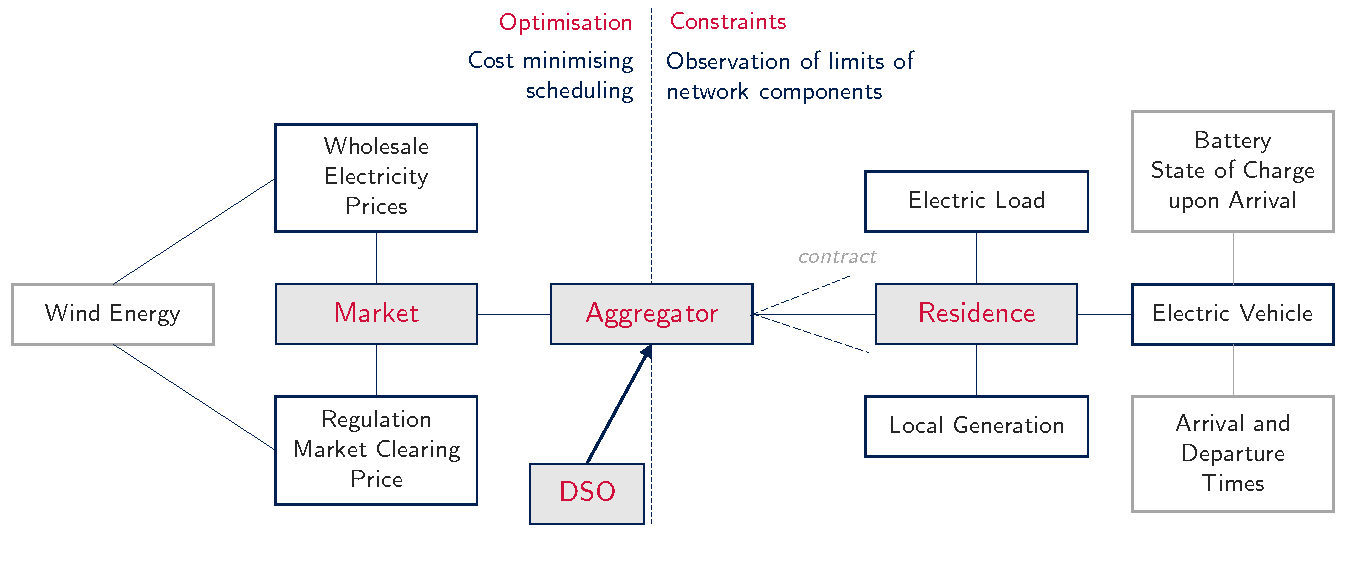
\includegraphics[width=0.9\textwidth,trim={0cm 0cm 0cm 0cm},clip]{figures/uncertainties/uncertainties.pdf}
	\caption{Overview of sources of uncertainty in EV scheduling}
	\label{fig:uncertainties}
\end{figure}

Day-ahead planning with the possibility to adapt charging schedules may be inevitable for market participation and finding the most efficient schedules. Meanwhile, the availability of electric vehicles is widely regarded as a key determinant of load shifting potential. While on an aggregate scale consumer behaviour is quite accurately predictable, forecasts on an individual level are prone to substantial deviations. A simple approach to circumvent this uncertainty is to enforce pre-set arrival/departure times by contractual obligations. Planning assumes fixed arrival and departure times. Even if the arrival times are stochastic, EV owners are often asked to specify their expected departure time and required battery charge to the aggregator for optimisation purposes \cite{Shi2011}. A relaxation of such constraints on users of electric vehicles could facilitate widespread adaptation of EV charging control, as besides preserving flexibility of use it omits inconvenient latency and diligence in communication. However, it also permits further uncertainty to the optimisation. To ensure a reliable battery charging processes, permitted uncertainty requires consideration by accurate prediction in conjunction with other, more inherent sources of uncertainty. As outlined in \Autoref{fig:uncertainties}, besides indeterminate arrival and departure times these are the battery charge levels on arrival, residential loads including the variability of local photovoltaic generation, and wholesale market prices influenced by the availability of large-scale renewable generators. Assessment of their impact on the performance of centralised charge control will be a principal contribution of this dissertation.

% other constraints / approaches
% -- Tesla power to provide link between local PV generation and EV charging -- investment? not everyone has PV but may use EV
%-- decentralised energy generation (PV), more independent power supply from the grid -- solution to both- more sustainable energy supply for EV demand and releasing local network strains

\subsection{Potential for Sustainable Electric Mobility}

% summary
In \cite{Daina2017} the preceding line of argument is shared and concisely summarised: ``\textit{On one hand electric grids capacity can be strained by an unmanaged EV load, especially at the distribution level where the capacity bottlenecks are most easily reached. On the other, if charging demand flexibility can be harnessed by implementing smart charging strategies, not only can costly grid capacity upgrades be minimised, but the operation of grid systems can be enhanced making use of a potentially very large responsive storage constituted by the batteries of grid-connected EVs.}''

% contribution
In short, electric vehicles can raise the share of renewable energy supply in a twofold manner if their charging processes are coordinated efficiently: first, they substitute fossil-fueled vehicles increasing the primary energy efficiency of the transport sector, and second, they facilitate the integration of renewable energy sources into the power grid via their load shifting capabilities.

\section{Research Questions and Objectives}
\label{sec:rq}

The primary goal of this dissertation is to develop a robust cost-minimising unidirectional day-ahead scheduling routine for charging electric vehicles overnight in residential low voltage distribution networks while observing local network, equipment and charging demand constraints in a stochastic environment under the participation in a wholesale electricity market. To build the stochastic environment in which residential electricity demand, market prices mirroring renewable energy supply and demand peaks, and the mobility behaviour of electric vehicle owners are uncertain, the secondary objective is to characterise and derive suitable models for inherent and conceded uncertainties incurred with the optimal scheduling of electric vehicles. Therefore, the contribution of this work is twofold: an \textit{optimisation study} complements the development of a stochastic \textit{simulation model}.

For the \textit{simulation model}, emphasis shall be put on investigating empirical uncertainty in the mobility behaviour of particular electric vehicle users to derive stochastic consumer behaviour about arrival and departure times as well as battery charge levels that not only addresses vagueness concerning the positioning of different user types but also uncertainty due to vehicle owners deviation from their predicted typical behaviour. This will facilitate the analysis of implications from relaxing commonly assumed contractual obligations for the consumers' EV availability and the aggregator's allocation of final battery state of charge. That is to assess how unexpected consumer behaviour limits the capability of a central scheduling entity to refill electric vehicle batteries.

The \textit{optimisation study} shall focus on the performance of multiple deterministic optimisation methods under uncertainty and approaches to mitigate the impact of individual prediction errors. It explores the possibility of attenuating the detrimental impact of uncertain parameters without the use of computationally complex stochastic programming techniques utilising critical information about parameter distributions and pre-specified degrees of conservatism. In addition to uniting consumer electricity bill savings with grid support through charge rate coordination, it aims to provide insight into the effectiveness and robustness of variants of analytical and heuristic approaches compared to na�ve reference optimisation methods, and the moderation between a customer's mobility requirements and cost savings. Furthermore, it should indicate financial benefits from participating in devised charging control schemes under today's and future market and tariff-design conditions to derive indicative policy recommendations for a frictionless transition to a sustainable electrified transport sector.

In summary, this work will address the following research questions:

\begin{enumerate}
	\item What are the major uncertainties involved in day-ahead scheduling of electric vehicles and how can they be modelled generically? In particular, how does limited knowledge on exact availability periods and battery charge levels limit the reliability of unaware scheduling approaches?
	\item How does the performance and robustness of analytical and heuristic scheduling methods compare despite uncertain inputs and how effective are proposed uncertainty mitigation options in reducing the number and severity of constraint violations?
	\item More accurately, what is the relative cost and benefit of increasing the robustness towards forecast deviations in day-ahead scheduling by applying increasing security margins to the deterministic optimisation approaches?
	\item How do tariff design and intra-day variance of prices affect the cost saving potential of devising charging control of electric vehicles to an aggregator with access to the wholesale electricity market?
\end{enumerate}

\newpage
\section{Dissertation Structure}

Having motivated the topic of electric vehicle scheduling and having defined the research questions of this work in \textbf{\Autoref{sec:intro}}, this dissertation consists of five further parts which are structured as follows:

\begin{itemize}
	\item \textbf{\Autoref{sec:found}} performs a literature review on previous approaches to electric vehicle charging coordination and categorises this work within the research field.
	\item \textbf{\Autoref{sec:model}} describes the simulation framework in which the EV scheduling is embedded and sequentially builds continuous models of required input parameters from empirical data including profound estimates of their uncertainties.
	\item In \textbf{\Autoref{sec:opt}} a deterministic optimisation problem for optimal EV scheduling in the stochastic environment is defined. It comprises an introduction to heuristic and analytical approaches implemented including simple reference optimisations and concludes with the introduction of multiple deterministic uncertainty mitigation concepts.
	\item In \textbf{\Autoref{sec:eval}} the configured optimisation methods and uncertainty mitigation approaches are evaluated in comparison to uncontrolled charging. Besides analysing resulting schedules, emphasis is put on the sensitivities of different degrees of conservatism in uncertainty mitigation and the impact of varying price spreads.
	\item \textbf{\Autoref{sec:concl}} provides a summary of results and answers obtained regarding the research questions, as well as an outlook on further research on the topic of EV scheduling.
\end{itemize}


\chapter{Foundations and Literature Review}
\label{sec:found}

This chapter provides an introduction to the academic literature on the grid integration of electric vehicles. \Autoref{sec:impact} focusses on impact assessments of uncontrolled EV loads on various power network levels and outlines the potential benefit of controlled EV loads. Consequently, \Autoref{sec:deterlr} deals with previous approaches to optimise EV charging processes and compiles a summary of the different objectives and scopes of EV scheduling. Because reliability and robustness despite numerous uncertainties in scheduling are a major concern, \Autoref{sec:stochlr} regards related work that elaborated on scheduling methods considering forecast deviations. Finally, \Autoref{sec:barr} sketches out why EV owners might be hesitant to procure electric vehicles and participate in devised charging control. It deduces the significance of high cost savings and demand satisfaction rates in EV scheduling for an accelerated, sustainable, and grid-wise benign market uptake of electric vehicles.

\section{Impact and Potential of Electric Vehicles in Power Networks}
\label{sec:impact}

% GENERAL
The adoption of EVs will introduce new demand patterns into the power network, and assessment of their impact has received much attention in research over the past decade. Reference \cite{OConnell2014} notes that a majority of EV charging will take place on low voltage unbalanced networks and consequently the distribution feeder is particularly affected and inevitably requires remediation \cite{Ochoa2012, Lakervi2007}. It is estimated that uncontrolled EV loads can be accommodated in low-voltage distribution networks up to penetration rates between 20\% and 30\% without major technical problems \cite{Taylor2009, Quiros-Tortos2016, Richardson2010}. It is further shown that network strains are most severe during periods of simultaneous charging of a vast number of electric vehicles and peak residential demand. Two comprehensive literature reviews on impact studies are published in \cite{Papadopoulos2012, Dubey2015}. They categorise three main areas of concern summarised in \Autoref{tab:concern}: electricity generation adequacy, equipment strain, and power quality.

\begin{table}[]
	\centering
	\begin{tabular}{@{}lll@{}}
		\toprule
		\textbf{Generation Adequacy}    	& \textbf{Equipment Strain}            & \textbf{Power Quality}    \\ \midrule
		\tabitem security of supply     	& \tabitem transformer life and safety & \tabitem voltage drops    \\
		\tabitem carbon intensity       	& \tabitem cable life and safety       & \tabitem phase imbalances \\
		\tabitem power reserve availability & \tabitem battery life                & \tabitem power losses     \\
		\tabitem distributed generation 	&                                      & \tabitem harmonics        \\ \bottomrule
	\end{tabular}
	\caption{Major areas of concern regarding an increasing number of uncontrolled EV loads}
	\label{tab:concern}
\end{table}

% POWER QUALITY

Power quality comprises multiple dimensions. \cite{Boulanger2011,Wu2011,Pillai2010} demonstrate detrimental impacts of uncontrolled EV loads on voltage profiles in low-voltage residential distribution networks. \mbox{\cite{Richardson2010} conduct} an impact assessment of varying penetration levels of electric vehicles and show that already for modest penetration rates between 20\% and 40\%  voltage alongside line loadings can exceed statutory limits and would force the DNO to curtail its energy supply. Besides voltage issues, \cite{Clement-Nyns2010} point towards increased power losses in distribution networks. The results are confirmed in \cite{Paudyal2011} and \cite{Papadopoulos2012} found line losses to be as high as 10\% for high EV penetrations. \mbox{\cite{Putrus2009} add} phase load imbalances and subsequently voltage imbalances to the list of power quality concerns, while \cite{Koyanagi1999} analyses the development of power system harmonics. Stochastic analyses in \cite{Leou2013} verify the results of the mostly scenario-based studies.

% EQUIPMENT STRAIN
Alongside \cite{Richardson2010}, \cite{Papadopoulos2012} report frequent cable and transformer overloads and estimate that equipment stress is even more critical than voltage violations. 
\cite{Gong2012} study how uncontrolled EV charging negatively affects transformer insulation life. Likewise, \cite{Gomez2002, Shao2009, Warweg2011} analyse overloading and deterioration of transformer life due to total harmonic distortion (THD) of battery charger currents.

% GENERATION ADEQUACY
Although insufficient generation adequacy is a commonly stated concern, \cite{Webster1999, Hadley2009, Kintner-Meyer2007} conclude that despite growing EV loads existing and planned generation capacities suffice to guarantee the security of supply. Nonetheless, \cite{Dubey2015} note that uncontrolled EV loads may entail a significant reduction in power reserve margins. In \cite{Marwitz2016, Rassaei2014} the grid impact of EV loads against the backdrop of long-term planning regarding network reinforcement is analysed and underline the prohibitive costs of upgrading network equipment.

% CONCLUSION
Most papers conclude that technical difficulties can be overcome by controlled charging, which is illustrated with more or less rigorous charging strategies and assumptions. Consensus exists that existing distribution networks can accommodate substantial penetration levels of electric vehicles if the majority of charging is restricted to slow charging rates in off-peak periods \cite{Richardson2012a}. While \cite{Schuller2015a} quantify the load flexibility of electric vehicles and attest significant degrees of freedom, \cite{Quiros-Tortos2016} show that a control algorithm with control cycles of up to 10 minutes successfully mitigates power quality and equipment strain problems. Noteworthily, networks driven by high shares of renewable energy were shown to gain the most system cost reduction \cite{Shortt2012}. This suggests that the exploitation of load flexibilities by remote scheduling bears the potential to turn EV loads from a burden to a facilitator for the grid integration of renewable energy even beyond the additional demand the widespread adoption of EVs incurs.

\section{Deterministic Approaches to EV Load Scheduling}
\label{sec:deterlr}

Consequently, a vast amount of research was already conducted on the intelligent coordination of EV charging to harvest demand flexibility. The literature comprises a multitude of optimisation objectives, constraints, techniques, hierarchies, and scenarios. Comprehensive literature reviews in \cite{Mukherjee2015, Rajakaruna2015, Tan2016a} provide detailed insights into related studies examining conceivable applications deterministically; i.e.\ their work focusses on the theoretical potential and abstracts from operational uncertainties involved.

Besides the question whether discharge capabilities of electric vehicles are profitable, often the different control and communication architectures in which scheduling is embedded are discussed. Broadly central and decentral scheduling approaches are to be distinguished, whereby hybrid hierarchical control schemes are also conceivable. 

\textit{Central control} arranges charging processes by direct load control through a central scheduling instance and primarily focusses on reliable and safe network operation \cite{Vaya2012, Schuller2013}. Although new scheduling algorithms would integrate well with existing power system control, privacy concerns due to high requirements for information exchange as well as poor scalability for complex optimisation procedures could be prohibitive \cite{Li2005, OConnell2014}. 

Conversely, \textit{decentral control} retains the charging control of EV owners. Based on price discrimination with respect to time and location owners decide on when and to what objective to schedule, while pricing mirrors the technical status of the distribution network \cite{Rajakaruna2015}. Compared to central control it requires only minimal communication infrastructure mitigating data protection concerns and primarily aspires to fulfil EV owners' desires \cite{OConnell2014}. Furthermore, the division of the scheduling problem into subsets aids the problem scalability. Consequently, a group of advocates of decentral charging control exists \cite{He2012, Contreras-Ocana2016, Xing2015, Gan2013}.

While the use of standard functions to solve mixed-integer linear and convex non-linear problems dominate the literature \cite{Wu2012,Akhavan-Rezai2016}, dynamic programming \cite{Han2010, Rotering2011} and meta-heuristics such as particle-swarm optimisation \cite{Hai-Ying2011, Arias2017, Peppanen2014, Soares2013,Celli2012, Wen2016} have received growing attention to solve scheduling problems more quickly and efficiently. Correspondingly, \cite{Sassi2016} compare the complexity between exact and heuristic methods.

%\subsection{Technical Objectives}

The literature review in \cite{Rajakaruna2015} organises optimisation objectives into technical, environmental and economic objectives. It acknowledges, however, that a sharp distinction between the categories is not always feasible.

\textbf{Technical objectives} primarily target to maintain safe grid operation despite EV loads and intermittent renewable energy supply. In the distribution system, applications for peak shaving and load reduction prevail \cite{Mets2010, Turker2013, Wang2013a}. Thereby, \cite{Lopes2010, Mets2010} could increase the number of tolerable EVs from 10\% to 52\% by reducing peak load by 40\%. Further research evolves around the minimisation of losses and equipment strain \cite{Deilami2011, Sortomme2011} or even reactive power compensation \cite{Tan2016a}. \cite{Acha2012} achieved a loss reduction by 25\% for evaluated scenarios by coordinated charging. In addition to remedying thermal line loadings, \cite{Sundstrom2012, Connell2012} aimed and succeeded at stabilising voltage levels in residential areas. Similarly, in \cite{Richardson2012,Richardson2012a} a maximisation of the toal amount of energy that can be delivered in a distribution network while ensureing that network and voltage limits are never exceeded due to high levels of coincident charging. The results are confirmed by \cite{Richardson2010, Huang2012} which additionally seek to minimise phase imbalances \cite{Richardson2012}.

Alternative strategies for superordinate transmission systems apply as \cite{Vaya2012, Salah2012} noted a discrepancy between system state of the distribution system and transmission system. Studies on the transmission system level focus on the unit commitment problem regarding the carbon intensity and operation costs on the generation site \cite{Kiviluoma2011, Sioshansi2009}. 

The vehicle-to-grid (V2G) was laid out by \cite{Kempton1997} and entails an increased need for communication infrastructure \cite{Quinn2009}. Controlled EVs provide ancillary services such as spinning reserve and frequency regulation support \cite{Lopes2010, Tomic2007, Andersson2010}. V2G services are naturally linked to revenue generation from energy feed-back, paid per unit of energy, and capacity reserve provision, paid by capacity and time\cite{Kempton2005a}. \cite{Dallinger2011, Sortomme2011} show that negative regulation, namely charging in energy surplus periods, is most profitable while positive regulation would require additional investments. In \cite{Peterson2010} it is further demonstrated that capacity services rather contains the detrimental impact on battery lifetime.

\textbf{Economic objectives} eclipse the technical benefit of V2G and prioritise profits \cite{Sortomme2012}. Many also seek to exploit the load shifting potential by minimising the procurement cost of required energy on ordinary wholesale markets. Thereby, technical constraints are often only considered on a system level given implicitly through the price-building mechanism. While \cite{Guo2016} show the financial benefit to providers of V2G services, \cite{Cao2012} demonstrate how optimised charging pattern has great benefit in reducing cost and flatting the load curve if the peak and valley time periods are partitioned appropriately. Caution is however required as purely price-responsive charging according to uniform pricing based on the wholesale market may entail new peaks of EV loads \cite{Flath2013}.

\textbf{Environmental objectives} are usually intertwined with economic and technical objectives, and target to remedy the impact of additional volatile renewables, reduce fossil fuel dependency and reduce greenhouse gas emissions. The classic goal is to increase the utilisation share of renewables when charging by coupling renewable generation with EV loads \cite{Richardson2013, Vandael2011} and predominantly focus on wind power integration \cite{Pehnt2011, Short2006, Denholm2006}. In \cite{Druitt2012} it is derived that in a scenario where 30\% of electricity in the UK is supplied by wind power, one million electric vehicles could provide half the required balancing power. This order of magnitude is verified in \cite{Ekman2011}. Study \cite{Goransson2010} achieved emission reductions and efficiency increases in thermal generation due to less frequent start-ups and part load operation as intermittency is moderated by electric vehicles. However, regarding V2G applications \cite{Kempton2005, Kempton2006} note that EVs can only provide short-term storage of less than 2 hours, but may not attenuate daily or weekly generation variation.

In conclusion, potential applications of coordinating the charge rates of electric vehicles are diverse, but market-based and network-based optimisation are often disjunct. That is, a cost-minimising algorithm may disregard network constraints, or a peak-shaving algorithm neglects potential economic benefits. 

\newpage
\section{Stochastic Approaches to EV Load Scheduling}
\label{sec:stochlr}

In light of the prevailing uncertainties, it further needs to be acknowledged that charging coordination is no static offline problem but must incorporate possible forecast errors already while optimising \cite{Aghaei2016}. As compiled in \Autoref{tab:unclr}, several papers have presented diverse approaches to tackle uncertainties in recent years primarily addressing spot market prices, intermittent renewable electricity production, and EV user behaviour individually. Other than deterministic scheduling methods, economic cost minimisation objectives dominate, although they may be intertwined with environmental objectives, for instance by targeting maximum self-consumption of renewables \cite{Mehri2017, Jin2014, Bai2015}. Further, the literature offers a broad range of solution methods and problem formulations evolving around receding horizon control, stochastic and robust optimisation. 

\textbf{Robust optimisation} is predominantly applied to hedge against uncertain spot market prices. \cite{Soroudi2014} develop a scheduling approach based on a bi-level robust optimisation formulation that is immune to worst-case price prediction errors up to a controlled degree of risk aversion while considering nonlinear power flow. \cite{Korolko2015} criticise their negligence of physical battery limitations and the tractability of the proposed formulation. Instead, they present a cutting plane method to achieve robust solutions on an unregulated electricity market considering the nonlinear state-of-charge curve of batteries. Using a mixed-integer quadratic programming model, \cite{Bai2015} underline the benefit of aggregators participating in regulation services by reducing the total cost of thermal generators and containing the uncertainty of network operation costs.

\textbf{Stochastic optimisation problems} have been solved by information gap decision theory \cite{Zhao2015, Al-Awami2012}, Lyapunov optimisation \cite{Zhou2017}, Markov decision processes \cite{Zhang2014, Shi2011} as well as Monte Carlo methods \cite{Wu2017,Al-Awami2012}, scenario tree reduction \cite{Mehri2017}, and dynamic stochastic optimisation \cite{Liu2017}. To solve the EV scheduling problem by a Markov decision process in conjunction with a \mbox{Q-learning} algorithm, \cite{Shi2011} model price uncertainty via a Markov chain with unknown transition probabilities. \cite{Zhao2015} could formulate effective strategies to guarantee a predefined profit for risk-averse aggregators and demonstrate the trade-off between desired profits and preferred risk levels. Complementary, \cite{Zhou2017} point out that for their algorithm, the trade-off between cost and average fulfilment ratio of charging requests is at most linear.

\textbf{Receding optimisation horizons} are employed in \cite{Wang2017, Vaya2015, OConnell2014} to allow using available knowledge of preceding periods and updated more accurate forecasts to adapt optimised schedules. Using sequential quadratic programming, \cite{OConnell2014} could achieve an effective reduction in forecast error impacts ascribed to a rolling optimisation horizon to limit the period of agnostic decision-making. In a decentralised scheduling approach, \cite{Vaya2015} utilise the alternating direction method of multipliers (ADMM) to mitigate user mobility uncertainty and emphasise the benefit of parallel computation of local optimisation problems for scalability. Receding horizon control is further employed in conjunction with virtual load constraints in \cite{Wang2017}. They use model predictive control (MPC) to mitigate stochastic user behaviour modelled by kernel-based estimators.

Three frequently neglected issues detected motivate the scope of this dissertation. First, among the papers addressing various domains of uncertainty, few focus on the technical constraints of distribution networks \cite{Mehri2017, OConnell2014, Soroudi2014}. This contradicts the argument in \Autoref{sec:impact} that particularly low-voltage networks are sensible to additional EV loads, and therefore, deserves more attention. Second, stochastic and robust optimisation problems add substantially to the complexity of solution methods. The question arises whether plainer deterministic optimisation procedures would facilitate the adoption of remote scheduling while achieving equal levels of robustness if conservative parameter estimates are employed. A literature review on \mbox{state-of-the-art} decision making under uncertainty in energy systems is provided by \cite{Soroudi2013b}. Their intricacy repeatedly appears to fuel the phenomenon that models are suited to allow a particular optimisation method and not vice versa. Third, the common focus on individual aspects of uncertainty and less extensive model scopes further limit the comprehensive and realistic modelling of the charging problem and impact assessment. Furthermore, the cost and benefit of robustness are only partially evaluated.

% Please add the following required packages to your document preamble:
% \usepackage{booktabs}
% \usepackage{multirow}
\begin{landscape}
	\begingroup
	%\fontsize{9pt}{10pt}\selectfont
	\small
	\singlespacing
	%\renewcommand*{\baselinestretch}{1.0}
	\begin{longtable}{@{}p{0.5cm} >{\raggedright}p{4cm} >{\raggedright}p{3cm} >{\raggedright}p{3cm}  p{0.2cm}  p{0.2cm}  p{0.2cm}  p{0.2cm}  p{0.2cm}  p{0.2cm}  p{0.2cm} >{\raggedright\arraybackslash}p{4cm}}
		\toprule
%		\multirow{2}{*}{Paper} & \multirow{2}{*}{Objective}                                                                            & \multirow{2}{*}{Problem / Model} & \multirow{2}{*}{Solution / Method}             & \multirow{2}{*}{Type} & \multirow{2}{*}{Grid Constraints} & \multicolumn{5}{l}{Consideration of uncertainty in optimisation}                                    & \multirow{2}{*}{Remarkable Findings}                                                                                     \\ \cmidrule(lr){7-11}
%		&                                                                                                                &                                           &                                                         &                                &                                            & Renewables & Res. Demand & EV demand & EV availability & Prices &                                                                                                                                   \\ \midrule
\rot{\textbf{Paper}} & \textbf{Research Objective} & \textbf{Formulation} & \textbf{Method} & \rot{\textbf{V2G}} & \rot{\textbf{Grid Constr.}} & \rot{\textbf{Renewables}} & \rot{\textbf{Demand}} & \rot{\textbf{Battery}} & \rot{\textbf{Available}} & \rot{\textbf{Price}} & \textbf{Remarkable Findings} \\ \midrule
\endhead

\rowcolor[gray]{.95} \cite{OConnell2014}                    & Minimise charging costs                                                                                        & Receding horizon                          & Sequential quadratic programming                        & $\times$                 & \checkmark                                        & $\times$                  & \checkmark                & \checkmark              & \checkmark                    & \checkmark           & Effective reduction of forecast error impacts through rolling optimisation                       \\

\cite{Wang2017}                        & Minimise charging costs                                                                                        & Receding horizon                          & Model Predictive Control                                & $\times$                 & $\times$                                         & $\times$                  & $\times$                   & \checkmark                & \checkmark                      & $\times$              & Proved benefit of utilising receding horizon control and virtual load constraints                                                 \\

\rowcolor[gray]{.95} \cite{Vaya2015}                        & Minismise cost of charging by decentralised control                                                            & Receding horizon                          & Alternating direction method of multipliers             & $\times$                 & $\times$                                         & $\times$                  & $\times$                   & \checkmark                & \checkmark                      & $\times$              & Scalable parallel computation of local optimisation problems                                     \\

\cite{Soroudi2014}                    & Minimise total operating costs of energy procurement in distribution networks.                                 & Bi-level robust optimisation              & SNOPT Solver                                            & \checkmark                  & \checkmark                                        & $\times$                  & $\times$                   & $\times$                 & $\times$                       & \checkmark             & Immunisation of schedule to prediction errors to a controlled degree of risk-aversion. \\%

\rowcolor[gray]{.95} \cite{Bai2015}                         & Minimise the total cost of all thermal generators and all PEV aggregators                                      & Robust optimisation                       & Mixed-integer quadratic programming               & \checkmark                  & $\times$                                       & $\times$                  & $\times$                   & \checkmark                & \checkmark                      & \checkmark             & Aggregators participating in regulation services benefit the power grid and contain the uncertainty of costs of network operation \\

\cite{Korolko2015}                     & Minimise charging costs in an unregulated electricity market                                                   & Robust optimisation                       & Cutting plane method                                    & $\times$                 & $\times$                                         & $\times$                  & $\times$                   & $\times$                 & $\times$                       & \checkmark             & Feasible and robust solutions are achieved close to optimality with respect to uncertain market prices                            \\

\rowcolor[gray]{.95} \cite{Zhao2015}                        & Guarantee a predefined level of charging costs                                                                 & Stochastic optimisation                   & Information gap decision theory                         & \checkmark                  & $\times$                                         & $\times$                  & $\times$                   & $\times$                 & $\times$                       & \checkmark             & effective strategies to secure a predefined profit for risk-averse decision makers                                               \\

\cite{Zhou2017}                        & Minimise charging costs at a charging station with deadline constraints.                                       & Stochastic optimisation                   & Lyapunov optimisation                                   & $\times$                 & $\times$                                         & \checkmark                 & $\times$                   & \checkmark                & \checkmark                      & \checkmark             & robust algorithm points out that trade-off between cost and average fulfilment ratio of requsts is at most linear                 \\

\rowcolor[gray]{.95} \cite{Jin2014}                         & Minimise the cost of drawing non-renewable energy from the grid                                                & Stochastic optimisation                   & Lyapunov optimisation                                   & $\times$                 & $\times$                                         & \checkmark                 & $\times$                   & \checkmark                & $\times$                       & \checkmark             & Robust reduced charging costs and delay of charging                                                                         \\

 \cite{Zhang2014}                       & Minimise average length of charging under an average cost constraint                                           & Stochastic optimisation                   & Markov decision process (MDP)                           & $\times$                 & $\times$                                         & \checkmark                 & $\times$                   & $\times$                 & \checkmark                      & \checkmark             & -                                                                                                                               \\

\rowcolor[gray]{.95} \cite{Shi2011}                         & Profit maximisation for EV owner by participation on a regulation service market                               & Stochastic optimisation                   & Markov decision process (MDP) with Q-Learning algorithm & \checkmark                  & $\times$                                         & $\times$                  & $\times$                   & $\times$                 & $\times$                       & \checkmark             & Model price uncertainty via a Markov chain with unknown transition probabilities                                                  \\

\cite{Al-Awami2012}                    & Maximize a load-serving entity's profits through V2G services while maintaining risks within acceptable levels & Stochastic optimisation                   & CVaR on mixed-integer stochastic linear programme       & $\times$                 & $\times$                                         & $\times$                  & $\times$                   & $\times$                 & $\times$                       & \checkmark             & V2G services help to lower LSE risk levels and reduce emissions by displacing thermal generation \\

\rowcolor[gray]{.95}  \cite{Mehri2017}                       & Minimise charging cost and emissions of EV charging                                                            & Stochastic scenario tree                  & MINLP with epsilon-constraint method                    & \checkmark                  & \checkmark                                        & \checkmark                 & \checkmark                  & $\times$                 & $\times$                       & $\times$              & Reliable benefit for both system operator and EV owner resulted from bidirectional scheduling.  \\

\cite{Wu2017}                          & Scheduling in public charging stations with distributed generation to minimise charging costs                  & Two-stage stochastic optimisation         & Monte Carlo sample-average approximation technique      & \checkmark                 & $\times$                                      & \checkmark                 & \checkmark                  & \checkmark                & \checkmark                      & \checkmark             & Benefits in reducing charging costs, detrimental influence on the distribution network, and unsatisfied charging demand           \\
		
\rowcolor[gray]{.95} \cite{Liu2017}                         & Minimise charging costs                                                                                        & Stochastic linear programme               & Dynamic stochastic optimisation                         & $\times$                 & $\times$                                         & \checkmark                 & $\times$                & \checkmark                & \checkmark                      & \checkmark             & Achieved near-optimal results                                                 \\		 \bottomrule
\caption[Literature review of stochastic scheduling approaches]{Literature review of stochastic scheduling approaches and which uncertainties they consider (\checkmark = yes / $\times$ = no )}
\label{tab:unclr}
	\end{longtable}

\endgroup

\end{landscape}
%\restoregeometry



\section{Barriers and Challenges to EV Emergence and Scheduling}
\label{sec:barr}

For designing an optimal EV scheduling algorithm identifying potential facilitators and prevalent barriers for both EV market uptake and owners' engagement with aggregators is pivotal. Several obstacles must be overcome for widespread grid-friendly EV adoption, whereby social and technical barriers are of equal importance. For an overview of challenges confer \Autoref{tab:barriers}.

According to a survey, the biggest social concerns about electric vehicles stem from high cost, limited battery range, battery degradation, reliability and charging infrastructure \cite{Egbue2012}. Especially, the high upfront investment cost provides a disincentive to acquiring electric vehicles, while range anxiety of users of electric vehicles is increasingly solved by the advent of modern Lithium-ion batteries \cite{Tan2016a}. The need to estimate the present value of fuel cost savings and devised charging control requires effort and yields indefinite results as estimates are based on a volatile market \cite{Sovacool2009}. It was moreover shown that compared to other domestic energy efficiency measures, electric vehicles exhibit long payback periods \cite{Sovacool2009}. But also non-financial factors such as doubt about the sustainability of electrified transport, risk-aversion and security concerns about an unproven technology and the general public perception play a vital role in shaping purchase decisions \cite{Egbue2012}.

When additionally taking remote charging control into account, further issues arise. A prerequisite of demand side management (DSM) is suitable local communication infrastructure to control distributed flexible loads, which is not widely available to date \cite{Budka2014}. Even if ICT infrastructure is provided, increasingly complex grid control (due to many tiny controllable units) and energy losses (due to storage and potential feed back to the grid) constitute a major challenge \cite{Strbac2008, Dehaghani2012}. Most importantly, the limits of usable load flexibility need to be addressed. Because the supply of ancillary services is not the primary purpose of electric vehicles, flexibility is constrained by reliably fulfilling the users' mobility demands \cite{Dehaghani2012}. 

% Please add the following required packages to your document preamble:
% \usepackage{booktabs}
\begin{table}[]
	\centering
	%\footnotesize
	\resizebox{\textwidth}{!} {%
		\begin{tabular}{@{}lll@{}}
			\toprule
			\textbf{Social barriers}                     & \textbf{Socio-technical barriers} & \textbf{Technical barriers}              \\ \midrule
			\tabitem high investment costs               & \tabitem driving range            & \tabitem lack of ICT infrastructure      \\
			\tabitem risk-aversion / security concerns & \tabitem battery degradation      & \tabitem complexity of network operation \\
			\tabitem privacy preservation                & \tabitem reliability              & \tabitem energy conversion losses (V2G)  \\
			\tabitem credibility of sustainability       & \tabitem regulatory framework     &                                          \\
			\tabitem sustainability awareness            &                                   &                                          \\
			\tabitem leniency and lack of simplicity     &                                   &                                          \\
			\tabitem public perception                   &                                   &                                          \\ \bottomrule
		\end{tabular}
	}
	\caption{Barriers and challenges to EV emergence and scheduling}
	\label{tab:barriers}
\end{table}

Consequently, the social question arises to what extent consumers are willing to contribute to the integration of electric vehicles plus renewable energy. Besides reliability issues, the utilisation of EV batteries for DSM is proven to accelerate battery degradation due to more frequent charge/discharge cycles and limit the usable battery capacity \cite{Peterson2010, Wang2013a}. Consequently, batteries must be replaced more frequently and participants must be reimbursed to make DSM attractive \cite{Dehaghani2012}. Reference \cite{Dutschke2013} conducted a survey asking participants for their preference regarding different tariff-schemes and charging control modes. While the largest group of participants favoured an extensive V2G-tariff with direct load control and bidirectional power flow yielding the greatest economic benefit, a similar amount of respondents preferred to adhere to single-rate tariffs. When asked about what would alter their decision to participate in devised charging schemes common factors were monetary compensation, the level of automation, and simplicity \cite{Dutschke2013}. A different study further highlighted concerns about privacy preservation due to the high degree of information exchange \cite{Sovacool2009}.

The studies underline that not sustainability but \textit{cost} and \textit{reliability} shape decisions to purchase EVs and engage in remote scheduling schemes. Thus, an economic not intrinsic drive to support the grid integration of renewables preponderates. In consequence, for a quick decarbonisation of the transport sector and customer acceptance of devised charging control, an aggregator should prioritise cost saving by wholesale market participation and demand satisfaction objectives under technical constraints, which optionally avoid control sequences detrimental to battery life.

%%% REGULATORY CONCERNS
%- "development of the regulatory framework needs to support more decentralized decisions and system operation, and must potentially be adapted to respond to structural changes imposed by the large numbers of distributed energy resources and adaptive loads like EVs" \cite{Schuller2013}
% - solutions: strong warranties, battery swap programs, increased tax credits, charging infrastrucutre investments
%- inappropriate market structure / lack of incentives
\addtocontents{toc}{\protect\newpage}
\chapter{Modelling and Statistical Analysis}
\label{sec:model}

% Why simulation.

Although first field tests and large-scale fleet trials aiming to develop recommendations for effective standardisation and charging management of electric vehicles have already been conducted e.g.\ in the projects CROME, iZeus, MeRegio in Germany \cite{Schauble2017}, the effort of testing experimental control and optimisation routines in physical systems is prohibitive; not least, because it includes interdisciplinary domains ranging from wholesale market participation to distribution network operation. Hence, it is common to turn to simulation to prove the resonance of novel optimisation approaches under varying market and network conditions.

A simulation is a valuable tool in domains, where real-world experiments are prohibitively costly, difficult to observe, or dangerous for technical equipment. It aims and succeeds at developing a better understanding of the problem at hand by replicating stylised patterns from real-world observations minted with the application of strategic behaviour on predicted parameters. Thereby, it can isolate the analysed problem from second-tier external influences.

The setting and scope of the developed simulation are pitched in \Autoref{sec:ssa}, while subsequent \Autoref{sec:sf} guides through the framework, the simulation study is implemented in. The meaningfulness of results obtained from any simulation highly depends on the quality of its inputs. Therefore, the models of individual input parameters are carefully introduced: \Autoref{sec:nt} gives an account of the used low-voltage test distribution network, while \Autoref{sec:rd} explains the generation and preprocessing of synthetic residential electricity demand profiles as well as its uncertainty representation. \Autoref{sec:ev} describes the choice of technical vehicle specification and provides an overview of possible charging system configurations. \Autoref{sec:tp} constitutes an essential part of modelling the uncertainty involved in EV charging coordination. Other than previous work it does not rely on historical data, but operates with continuous distribution fits for a user's expected average characteristics as well as typical deviation from this average, and is an addition to the research area. Ultimately, \Autoref{sec:ep} concludes the model with a representation of an adapted spot market for power trading.

\section{Setting and Scope of Analysis}
\label{sec:ssa}

Naturally, the scope of a simulation study mimicking complex systems is limited by its implementation and conjectures. To facilitate the classification of the presented study into related work on EV charging coordination, major assumptions and boundaries are summarised in the following bullet points:

\begin{itemize}
	\item Charging is exclusive to periods between the end of the last trip of the day and start of the first trip of the next day. 
	\item Charging occurs overnight at home, not at work. A particular focus lies on suburban low-voltage distribution networks without industrial loads.
	\item The penetration of electric vehicles in the network is 100\%. Of the 55 households considered, each has one electric vehicle.
	\item Charging control of private electric vehicles is devised to one central aggregator. Inter-aggregator communication and influences on the transmission system are omitted.
	\item The aggregator commands a sufficient number of electric vehicle to participate on a intra-day wholesale electricity market, but schedule day-ahead for coordination purposes. Other than day-ahead market participation, this keeps the option for instantaneous or repeated schedule adaptation in reaction to forecast deviations open.
	\item The aggregator schedules according to a charging cost minimisation problem under user satisfaction and technical constraints. It abstracts from the provision of ancillary services through discharging and is restricted to load shifting services only.
	\item Optimisation is performed on discrete time steps with a 15 minute resolution. Thereby, the actual control of network elements (e.g.\ OLTCs) and actual load and renewable generation intermittency is neglected.
	\item The optimisation horizon is 24 hours and optimisation is triggered daily at 1 pm. This time corresponds to the lowest availability probabilities of electric vehicles.
	\item Consequently, each vehicle entails 96 decision variables for each time slot within 24 hours, which represent continuous charging powers, constant within each time slot.
	\item Models and uncertainties in electricity price, residential electricity demand, EV availability, and daily distance travelled are represented by continuous distribution functions. In reality, this idealised representation would be substituted by more accurate information based on empirical behaviour logs of one specific customer and enquiries by user interfaces.
\end{itemize}

More detailed model assumptions designs are provided in the respective subsequent sections.

\section{Simulation Framework}
\label{sec:sf}

% Target

As outlined previously, consideration of uncertainties about EV scenarios is more prevalent in related work than the recognition of individual uncertainties in mobility patterns \cite{Soares2011, Dallinger2010a}, residential demand and market prices. The composed simulation framework seeks to unite both aspects: it comprises Monte Carlo analysis to cope with scenario uncertainty regarding the allocation of consumer types and general market conditions, while it also addresses the second-tier operational uncertainties.

% optimisation routine

The routine of the simulation study is structured as shown in \Autoref{fig:optroutine}:  After retrieving general parameters such as optimisation horizon, resolution of discrete time steps, starting time index, algorithm choice and parameters, the scenario is stochastically generated comprising behavioural as well as market models. In consequence, scenarios describe the model parameters of imaginable nights in which vehicles are scheduled on the same test network. It is important to note that a scenario refers to the allocation of e.g.\ certain user \textit{characteristics} in the network but not to the \textit{realisation} of uncertainties defined by the user type. Should information about voltages and line loadings in the distribution network be approximated by linear power flow, corresponding network sensitivities are determined beforehand and will be valid for all scenarios based on the same test network.

\begin{figure}[tp]
	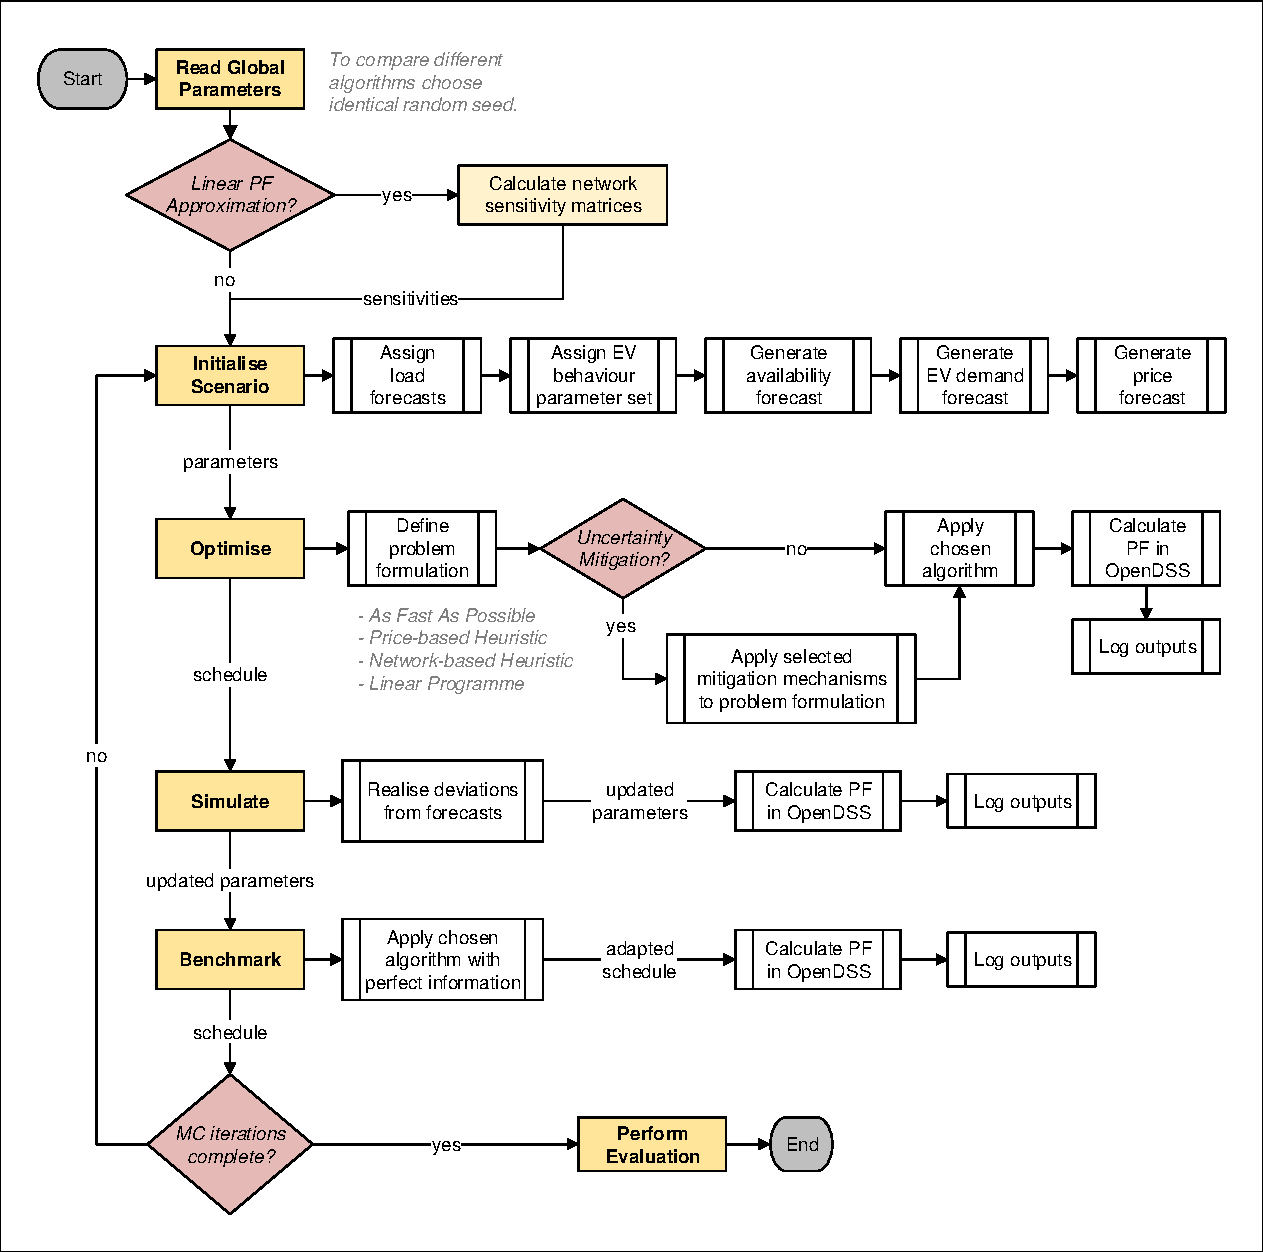
\includegraphics[width=\textwidth,trim={0.5cm 0.5cm 0.5cm 0.5cm},clip]{figures/framework/optimisationroutine}
	\caption{Flow Chart of Optimisation Routine in Simulation Framework}
	\label{fig:optroutine}
\end{figure}

The assessment of a scheduling approach for a specific scenario is based on three stages: the \textit{optimisation} schedules and coordinates EV charging processes according to the selected problem formulation, algorithm, and uncertainty mitigation options based on the forecasted parameters. Subsequently, the \textit{simulation} realises deviations from these forecasts in accordance with their uncertainty models and determines performance measures such as charging costs, fulfilment of customer demands, and observation of network constraints of the original optimised schedule. To compare these results to the optimal schedule that could have been achieved with the same algorithm had all the parameters been known \textit{ex ante}, the  \textit{benchmark} stage applies the selected algorithm with perfect information. In conjunction with the simulation results, the robustness of the optimisation algorithm to uncertainty can be assessed.

% Monte Carlo

Different optimisation algorithms and reference cases are evaluated relative to each other by running the same framework with identical parameter sequences. Because performance analysis of algorithms in a single scenario is inexpressive, the optimisation routine is coupled with a Monte Carlo (MC) simulation as applied in \cite{Navarro2013a, Navarro2013}. Arbitrary circumstances may favour one algorithm over another and, thereby, warp the evaluation. To hedge against this randomness, a series of scenarios are generated stochastically forming the basis of comparative performance assessment. Due to the multitude of scenarios optimised, a more accurate evaluation through distributions of performance measures is attained. Note that here the Monte Carlo simulation wraps the optimisation cycle and is not a component within the optimisation routine as used in e.g.\ \cite{Sandels2010}. Applied optimisation algorithms are exclusively deterministic. The many stochastic input parameters are entered either with their true expectation values or adapted through more conservative estimates.

% software architecture

The simulation framework has been implemented with an object-oriented approach in Python interfaced with the open source simulation tool OpenDSS to enable fast power flow (PF) studies of electrical distribution systems \cite{Ochoa2015}. OpenDSS origins from work by the Electric Power Research Institute and facilitates script-driven serial power flow simulations throughout a day in addition to snapshot analyses, pivotal to the impact evaluation of electric vehicle scheduling. Moreover, a series of IEEE test feeders are readily implemented in OpenDSS. It runs a three-phase unbalanced load flow using input data defined in \Autoref{sec:nt}.

\section{Network Topology}
\label{sec:nt}

Among the provided test distribution networks, the IEEE European Low Voltage Test Feeder developed in OpenDSS has been selected \cite{unknown2015}. Some studies focus on mitigating aggregated EV impacts in MV distribution networks \cite{Galus2011,GonzalezVaya2015a,Schwerdfeger2012}, but heavily loaded LV European distribution networks are likewise prone to technical issues caused by a market uptake of electric vehicles \cite{Quiros-Tortos2016}. Other than MV distribution networks, LV networks were traditionally designed with a \textit{fit and forget} attitude with little attention paid towards monitoring and operations management beyond power flows from the substation transformer. The penetration of low-carbon technologies demand a more active management approach towards low-voltage distribution circuits to avoid excessive voltage deviations, the transgression of thermal line limits, and phase unbalances of electric loads \cite{Ochoa2012}.

Many of the IEEE test cases are focused on North American 120/240 V single-phase distribution networks. Typically, these are characterised by an extensive MV system and a simple LV network, where there are only a handful of households connected to one transformer. However, European networks differ significantly as they consist of much simpler MV networks and more complex LV network structures \cite{Heinrich2012}. Fewer MV/LV transformers connect many more households via 230/400 V three-phase cables. Radial and meshed layouts are the two principal types of distribution grids. Meshed networks are prevalent in urban areas and possess multiple connections to the MV grid with interlinked feeders to hedge against the risk of outages due to maintenance operations or faults \cite{Ochoa2012}. Radial networks are more typical of rural and suburban areas. Their tree-shaped layout with a central connection to the MV network branching towards individual households is characteristic of the IEEE European Low Voltage Test Feeder. Therefore, the study will focus on suburban European distribution networks and resembles distribution networks modelled in related works \cite{Melhorn2017, Navarro-Espinosa2014, OConnell2014, Connell2012, Quiros-Tortos2016, Richardson2012a}. 

The radial distribution feeder operates at a line-to-line voltage of 400 V and a base frequency of 50 Hz. It is connected to the MV system through an 11/0.4 kV transformer at one central substation. The three-phase transformer is generously rated at 0.8 MVA with a delta/grounded-wye connection and does not provide any tap-changing capability. The MV network is modelled as an 11 kV voltage source with an impedance specified by three-phase and single-phase short circuit currents at 3 kA each. The main feeder and laterals amount to 905 three-phase lines connecting 906 buses, whose characteristics are defined by line codes including sequence impedances and admittances and lengths. Because the test feeder originally does not provide values for line ampacities, these have been acquired from a LV capacitor placement study by Electricity North West \cite{ENWL2013}. 

\begin{figure}[tp]
	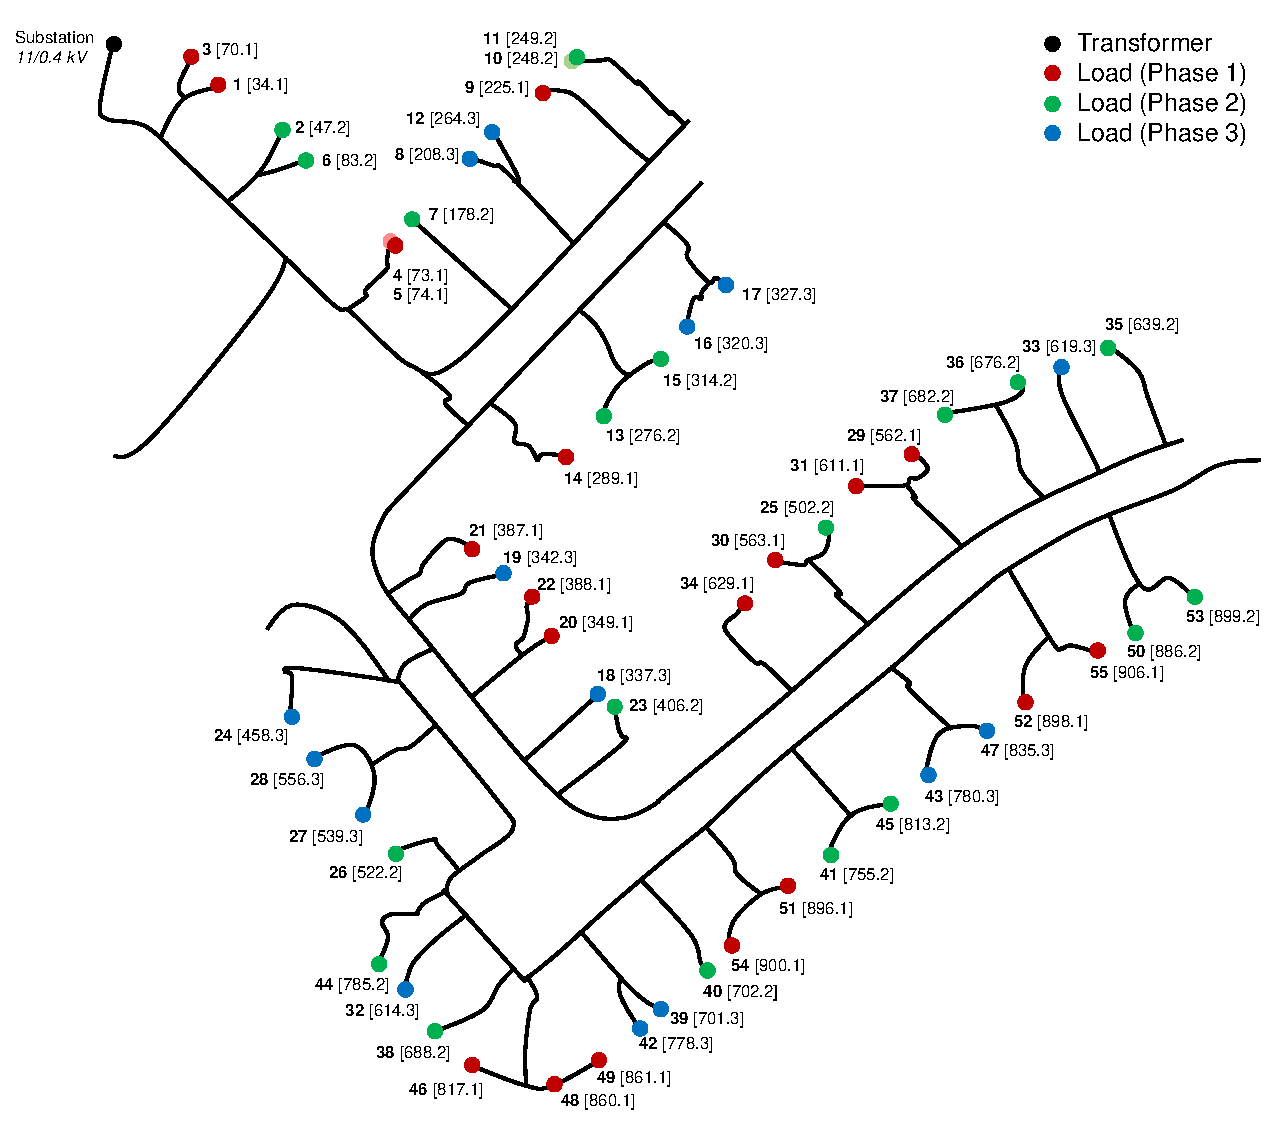
\includegraphics[width=\textwidth,trim={0cm 0cm 0cm 0cm}, clip]{figures/network/network_layout.pdf}
	\caption{Network topology and load locations of IEEE European low voltage test feeder}
	\label{fig:network}
\end{figure}

A geographical single-line diagram of the network is depicted in \Autoref{fig:network}. The test network comprises 55 numbered households connected to a single phase. The loads are rather evenly spread across the phases with 20 homes connected to each, phase 1 and phase 2, and 15 households attributed to phase 3. For simplicity, no further loads by industrial customers nor local photovoltaic generation are considered in the network.

% \cite{Bohn2017} 

\section{Residential Demand}
\label{sec:rd}

% Why?
Evaluating the functionality and impact of EV scheduling schemes in the low-voltage distribution network requires not only knowledge of EV loads but also a detailed insight into the spatial and temporal occurrence of residential loads. Considering high-resolution demand profiles that represent the variability of individual demands enables a comprehensive modelling of the network state and sensitivities to additional EV loads \cite{McKenna2016}. 

\subsection{Modelling}
% Generation of pool
A pool of 1000 individual residential electricity demand profiles, from which the stochastic scenario generation can choose, was created with the commonly used CREST demand model developed at Loughborough University \cite{Richardson2011}. Taking into account multiple factors such as the type of day, season, geographical location, and the number of occupants, it builds synthetic residential loads from individual devices and consumption activities. Consumer behaviour is modelled by Markov chains whose transition probabilities are derived from time-use surveys \cite{Richardson2010a,Richardson2008}. The output is a realistic 1-min resolution profile for domestic electricity demand of UK customers. 

To capture the sensitivity of residential loads to the number of active inhabitants in a household, the 1000 profiles were generated considering the proportion of homes with a given number of residents in the UK \cite{Figueiredo2005}. Households with one, two, three, four and five inhabitants are represented with 34\%, 40\%, 14\%, 9\% and 3\% respectively. More detailed clustering for load forecasts has been undertaken but is omitted for the sake of exposition \cite{Wu2007,Sousa2009}.

% Assumptions
Each household in the test network was assumed to maintain a constant inductive power factor of 0.96. For simplicity, no seasonal electricity demand variation is considered. Without loss of generality, the load profiles are confined to typical weekdays during winter capturing maximum demand in the UK. Furthermore, while some constituents of the residential demand might be deferrable and could be used for demand-side management, they are considered to remain static loads. 

% Assignment
For the stochastic scenario generation, electricity demand profiles were randomly assigned to each single-phase customer in the test distribution network. As the optimisation starts midday but the stored patterns are ordered from 0:00 am to 11:59 pm, the profiles are shifted by their difference of start indices. The adopted profiles are then resampled to match the chosen resolution of the optimisation routine. It is important to note that reducing the resolution will underestimate the temporal variability and, thereby, spoil the representation of instantaneous demand peaks as illustrated by three exemplary individual demand profiles for varying resolutions in \Autoref{fig:ind15min}, \Autoref{fig:ind5min} and \Autoref{fig:ind1min}.

\begin{figure*}[tp]
	\centering
	\begin{subfloat}
		\centering
		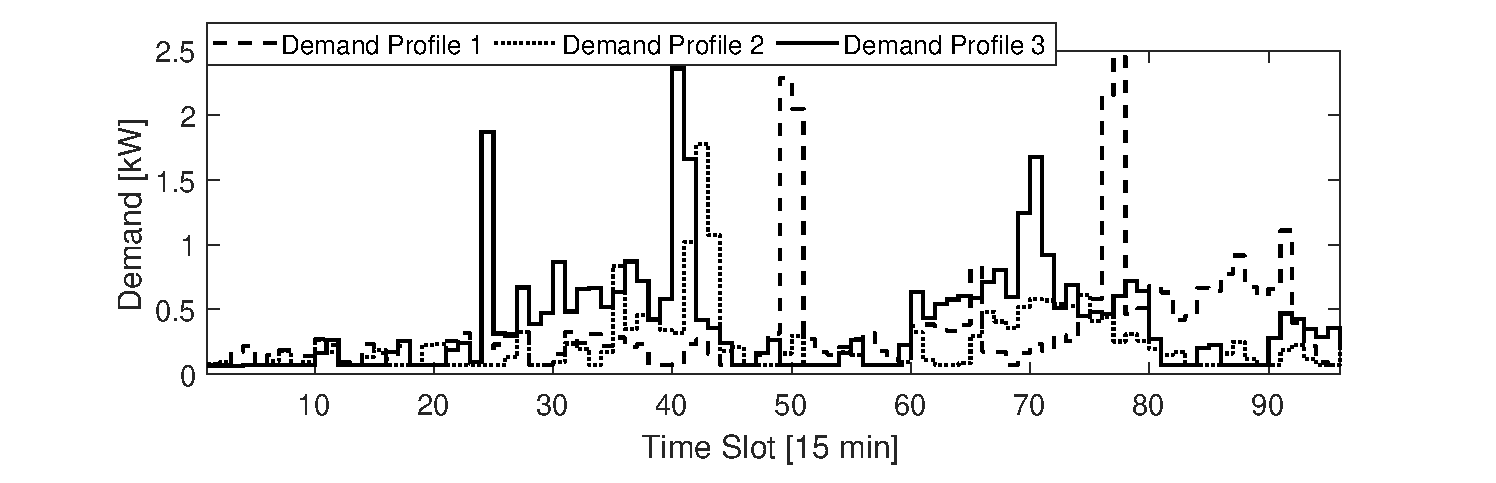
\includegraphics[width=.76\textwidth,trim={3cm 0cm 3cm 0cm}]{figures/demand/15minind.eps}
		\caption{Exemplary residential demand profiles 15-min resolution}
		\label{fig:ind15min}
	\end{subfloat}%
	\begin{subfloat}
		\centering
		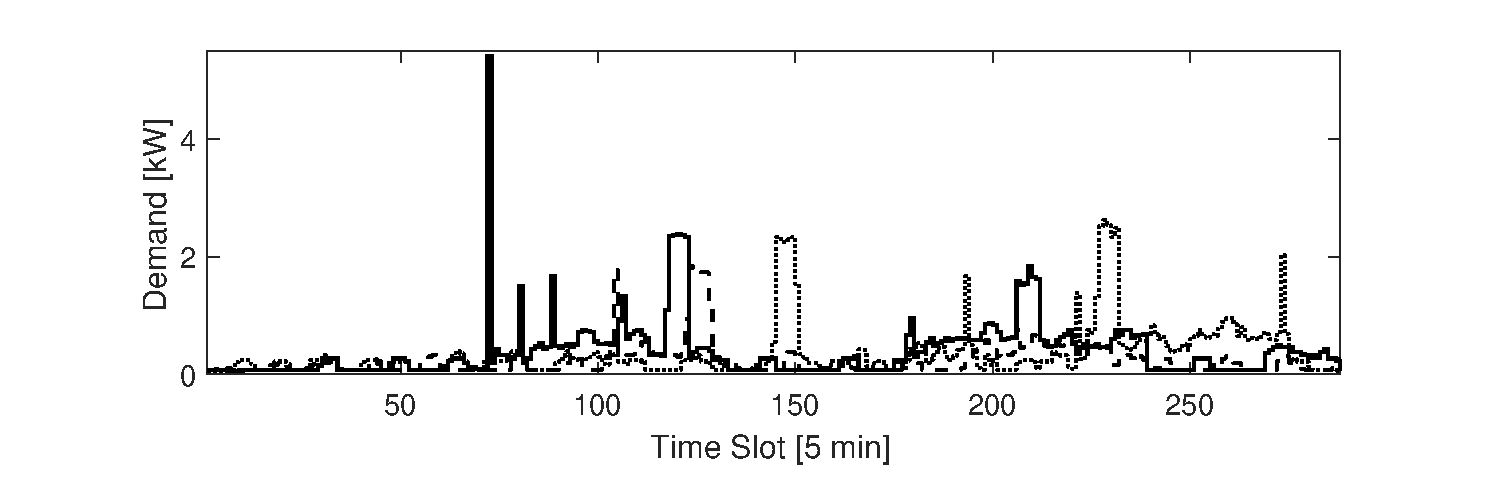
\includegraphics[width=.76\textwidth,trim={3cm 0cm 3cm 0cm}]{figures/demand/5minind.eps}
		\caption{Exemplary residential demand profiles 5-min resolution}
		\label{fig:ind5min}
	\end{subfloat}
	\begin{subfloat}
		\centering
		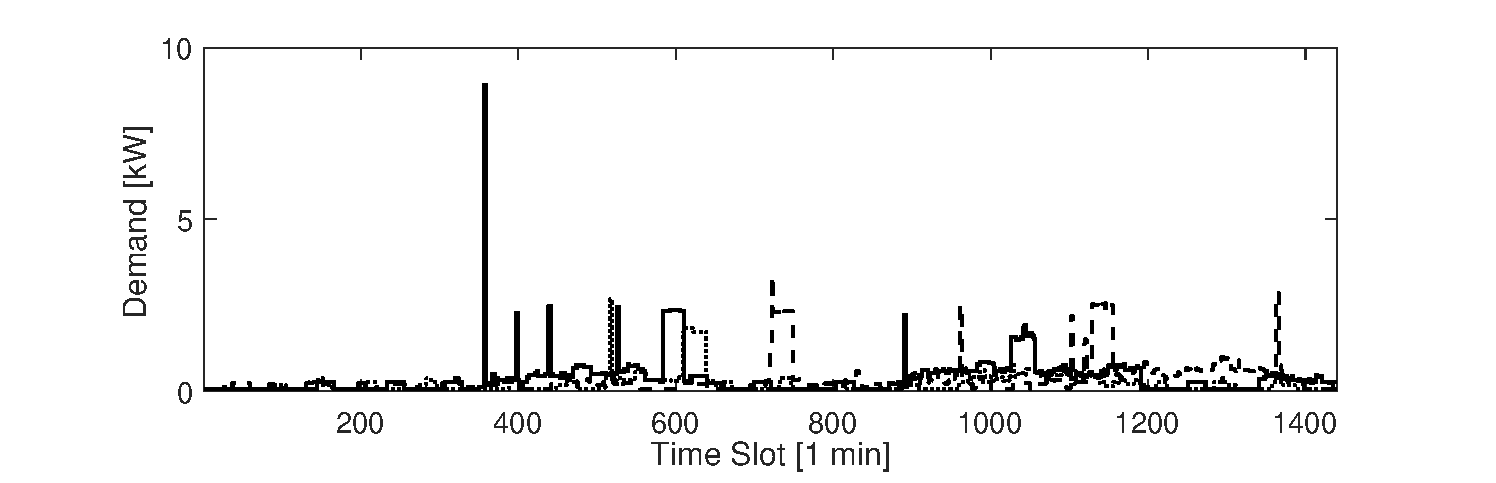
\includegraphics[width=.76\textwidth,trim={3cm 0cm 3cm 0cm}]{figures/demand/1minind.eps}
		\caption{Exemplary residential demand profiles 1-min resolution}
		\label{fig:ind1min}
	\end{subfloat}
\end{figure*}

% Figures
\Autoref{fig:demandboxplots} depicts the distribution spread of loads at each time slot via box plots highlighting both temporal correlation and the diversity of the time series. Aggregating all stored synthetic demand profiles and a comparison with the normalised ELEXON standard load profile \cite{ELEXON2017} for unrestricted domestic customers as shown in \Autoref{fig:aggregatedemandd}, confirms the approximate validity of the pool of load profiles.

\begin{figure}[tp]
	\centering
	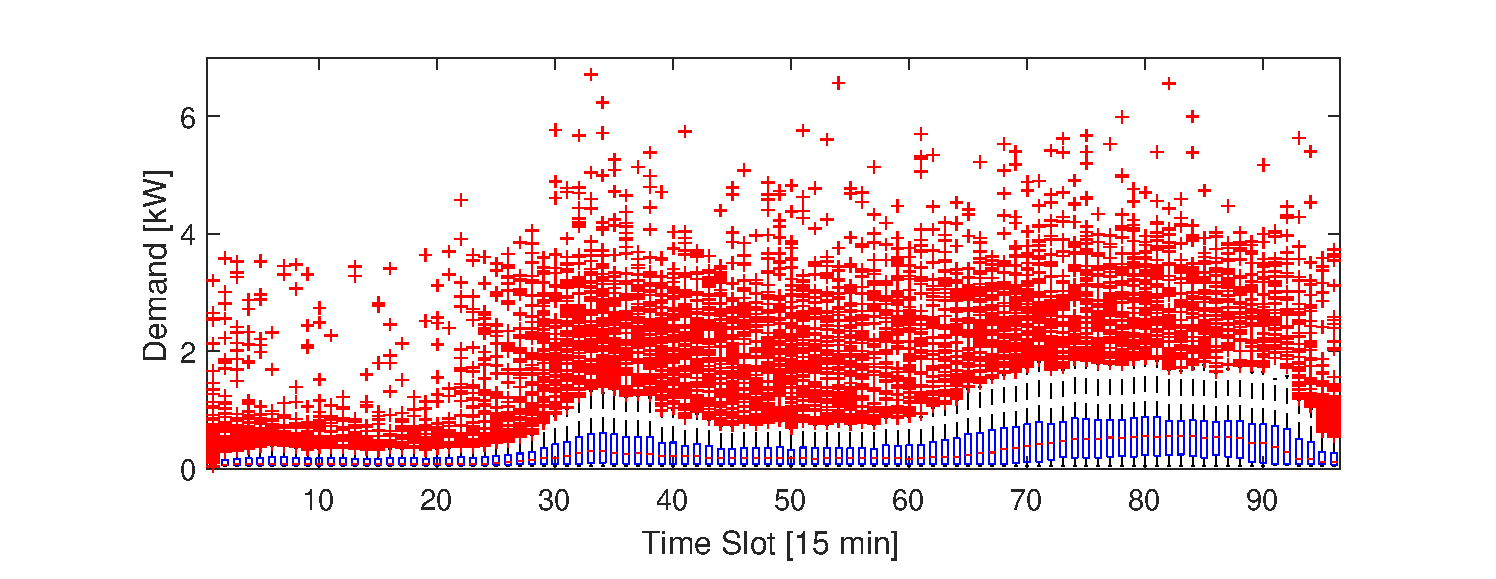
\includegraphics[width=.9\textwidth,trim={2cm 0cm 2cm 0cm}, clip]{figures/demand/indbox.eps}
	\caption{Boxplots of individual electricity demands}
	\label{fig:demandboxplots}
\end{figure}

\begin{figure}[tp]
	\centering
	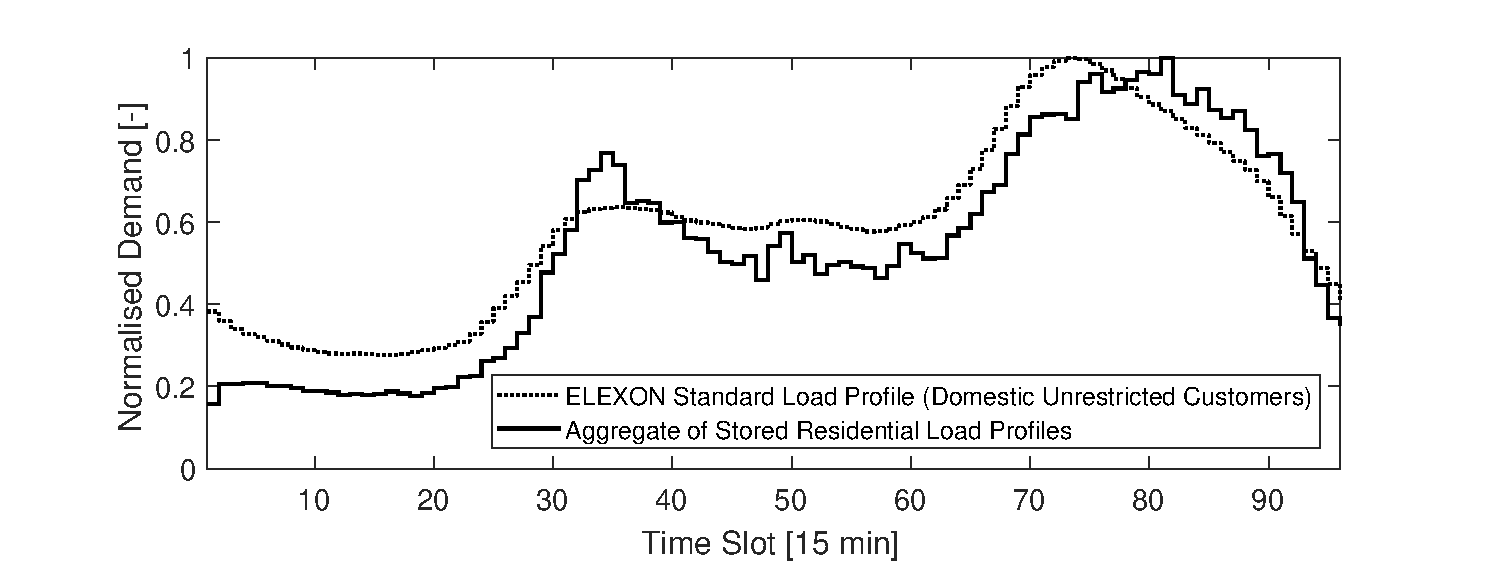
\includegraphics[width=.9\textwidth,trim={1.5cm 0cm 2cm 0cm}, clip]{figures/demand/aggdemand.eps}
	\caption{Aggregate electricity demand of stored profiles versus ELEXON average load profile}
	\label{fig:aggregatedemandd}
\end{figure}

\subsection{Uncertainty Representation}
\label{sec:rd_unc}

% Uncertainty
While on an aggregate scale consumer behaviour is quite accurately predictable, predicting individual behaviour is prone to substantial inaccuracies despite elaborate forecasting techniques \cite{Bandyopadhyay2015,Nguyen2015,Gajowniczek2017,Sevlian2014a,Riaz2007}. Multiple dimensions of uncertainty may be considered in terms of residential electricity demand; namely \textit{whether}, \textit{when}, and \textit{what amount} of electricity is required at an individual households. 

With smart metering infrastructure at the household level becoming increasingly available, more insight is obtained about the \textit{amount} of powers required in certain time frames \cite{Flath2012,Figueiredo2005}. While the exact time of an activity with a particular power demand heavily depends on customer behaviour, the prediction of the magnitude of this activity is less insecure. Most significant appliances are used on a regular basis and exhibit characteristic power signatures. Hence, deviations of simulated power demand magnitudes from their predictions are neglected.

Moreover, the uncertainty \textit{whether} a characteristic load is a second-tier problem. First, if the conservative default assumption is that an appliance is used, then unexpectedly not using this device will rarely lead to voltage or line loading problems in a heavily loaded distribution network and only marginally block network capacity for EV loads. Second, many typical cases where appliances are not used against typical behaviour -- such as holidays -- may be queried by a user interface releasing additional network capacity for EV loads.

Consequently, the uncertainty representation of residential electricity demand concentrates on \textit{when} characteristic household-level demand peaks occur. Although the deviations in the timing of different characteristic demand peaks throughout the day are likely to be independent, for simplicity they are modelled to be perfectly correlated. Thereby, the uncertainty of the demand forecast can be represented by shifting the simulated time series by a random duration. Let $w$ be the realisation of the random variable $W\sim \mathcal{U}(-w_{max},w_{max})$ denoting the uniformly distributed temporal deviation of the demand forecast $\hat{D}_t$ from the simulated demand $D_t$ within the maximum deviation $w_{max}=0.5$ h. Then the relation of predicted and simulated demand is given by

\begin{equation}
\hat{D}_t = D_{(t+w)\;\text{mod}\; T} \qquad \forall t\in T
\end{equation}

where the modulo operator assures that a continuous rolling maximum can be provided for the margins of the optimisation horizon.

\section{Electric Vehicles}
\label{sec:ev}

\subsection{Technical Vehicle Specifications}

\begin{table}[tp]
	\centering
	
	\begin{tabular}{@{}lllll@{}}
		\toprule
		\textbf{Vehicle Model}               & \textbf{Curb Weight}    & \textbf{Range}           & \textbf{Battery Capacity} & \textbf{Consumption}    \\ 
		& {[}kg{]}       & {[}km{]}        & {[}kWh{]}        & {[}kWh/km{]}   \\ \midrule
		Citro�n C-Zero              & 1,110          & 150             & 16               & 0.107          \\
		Karabag Fiat 500 E          & 2,340          & 130             & 28               & 0.215          \\
		Ford Transit Electric       & 1,120          & 140             & 20               & 0.148          \\
		Mercedes A-Class E-Cell     & 1,591          & 255             & 36               & 0.141          \\
		Nissan Leaf                 & 1,520          & 160             & 24               & 0.15           \\
		Peugeot iOn                 & 1,110          & 150             & 16               & 0.107          \\
		Renault Fluence Z.E.        & 1,610          & 185             & 22               & 0.119          \\
		Renault Kangoo Z.E.         & 1,410          & 170             & 22               & 0.129          \\
		Renault Zoe                 & 1,392          & 210             & 22               & 0.105          \\
		Smart Fortwo Electric Drive & 975            & 140             & 18             & 0.126          \\
		Tesla Roadster              & 1,220          & 393             & 53               & 0.135          \\
		Think Global Th!nk City     & 1,038          & 160             & 23               & 0.144          \\
		Tesla Modell S              & 2,108          & 335             & 60               & 0.179          \\
		Toyota RAV 4 EV             & 1,830          & 160             & 42               & 0.261          \\
		BMW i3                      & 1,315          & 183             & 33               & 0.169          \\ \midrule
		\textit{Average}            & \textit{1,446} & \textit{194.73} & \textit{29.01}   & \textit{0.150} \\ \bottomrule
	\end{tabular}
	\caption{Technical data of selected currently marketed electric vehicles \cite{Schuller2013,Salah2012,DepOfTrans2017} }
	\label{tab:evspec}
\end{table}

The relevant characteristics for modelling EV loads are the consumption rate, battery capacity and maximum range. A survey of the currently marketed electric vehicle produced the compilation of EV specifications in \Autoref{tab:evspec}. The list includes the top fully electric models of ultra-low emission vehicles (ULEV) registered for the first time in the UK in 2016 and commonly used reference vehicles in the literature \cite{DepOfTrans2017}. Noting a recent trend of increasing battery size and electricity consumption, the model assumes a single consumption rate of $\zeta=0.17$ kWh/km and a capacity of $B_{max}=30$ kWh for all modelled electric vehicles. Thereby, the consumption rate $\zeta$ creates a direct correspondence between battery capacity and vehicle range, although in reality using a singular value is a simplification; the amount of energy that an electric car consumes depends on a number of external factors such as the ambient temperature, driving speed, and the height profile of the covered track. Furthermore, neither battery degradation nor losses from storing electricity are considered in the technical EV model.

\subsection{Charging System Specification}

Details on charging infrastructure for the grid connection of electric vehicles encompass two major aspects: the physical network connection as well as communication and control ability. A multitude of connector types and charging modes exist differing in voltage and current levels, the number of phases or the type of connectors used. Which specifications prevail is largely dependent on the historical developments and traditions of both, distribution network operators and vehicle manufacturers \cite{Bossche2010}. Particular differences in specifications, as well as terminology, are noted between the USA and European countries. Regardless of location, conductive charging methods using cables and plugs can be distinguished from inductive methods transferring power magnetically. The former is current standard for EV grid connection and, thus, at the focus of subsequent analysis. Charging \textit{modes} summarise standards of connection specifications and infrastructure requirements, whereas charging \textit{levels} give a broader notion of power ranges with charging levels 1, 2, and 3 used in the context of US power systems and their European equivalents standard, semi-fast, and fast. An overview of charging modes, levels, plugs and their specifications is provided in \Autoref{tab:chargingmods}.

% Please add the following required packages to your document preamble:
% \usepackage{booktabs}
% \usepackage{multirow}
\begin{table}[tp]
	\centering
	\resizebox{\textwidth}{!} {%
	\begin{tabular}{@{}lllllll@{}}
		\toprule
		\textbf{Charging}          & \textbf{Charging} & \textbf{Charging}  & \textbf{Phases}  & \textbf{Voltage} & \textbf{Current} & \textbf{Power}    \\ 
		\textbf{Mode}              & \textbf{Levels}   & \textbf{Plug}      & \textbf{{[}-{]}} & \textbf{{[}V{]}} & \textbf{{[}A{]}} & \textbf{{[}kW{]}} \\ \midrule
		\multirow{5}{*}{Mode 1, 3} & EU Standard       & CEE7 / Type 2      & 1                & 230              & 16               & 3.7               \\
		& EU Semi-Fast      & Type 2             & 1                & 230              & 32               & 7.4               \\
		& EU Semi-Fast      & Type 2             & 3                & 400              & 16               & 11.1              \\
		& EU Semi-Fast      & Type 2             & 3                & 400              & 32               & 22.2              \\
		& EU Fast           & Type 2             & 3                & 400              & 63               & 43.6              \\ \midrule
		Mode 1, 2                  & US Level 1        & Nema 5-20 / Type 1 & 1                & 120              & 15               & 1.8               \\
		Mode 2, 3                  & US Level 2        & Type 1             & 1                & 240              & 30               & 7.2               \\ \midrule
		\multirow{2}{*}{Mode 4}    & US Level 3 DC     & Type 4 / CHAdeMO   & -                & 50-500           & 100              & 50                \\
		& EU Fast DC        & Type 2 Combo       & -                & 500              & 140-200          & 70-100            \\ \bottomrule
	\end{tabular}
	}
	\caption{Charging modes, levels, plugs and their specifications for $\cos\phi=1$ (adapted \cite{Bossche2010, Yilmaz2012, Schuller2013})}
	\label{tab:chargingmods}
\end{table} 

\textbf{Mode 1} refers to the direct connection of electric vehicles to AC networks with standard socket outlets, which do not exceed 16 A. Despite comparably low power levels, it can provide adequate energy for overnight charging. Mode 1 uses non-dedicated infrastructure for private premises that is readily available, which makes it the cheapest and most common approach. However, mode 1 does not employ protective equipment, particularly for EVs nurturing safety concerns. The sole protective elements used are a fuse or circuit breaker against overcurrents, earthing connection and, depending on the age of a building, residual current devices (RCD) to avoid detrimental leakage currents. 

\textbf{Mode 2} also uses standardised sockets but adds further protection via a control box with a control pilot conductor between vehicle and plug \cite{Bossche2010}. Although it remedies some safety concerns, it is restricted to cable protection and disregards the plug itself which may be more liable to damages during operation. Moreover, no communication protocols for control purposes are enabled.

\textbf{Mode 3} defines the direct grid connection of electric vehicles to the AC network utilising dedicated EV supply equipment \cite{Schuller2013}. According to the IEC Standard 61851-1, it mandates control pilot protection applied to enable continuous control and charge rate modulation. Its roles are summarised in \cite{Bossche2010} in four categories as

\begin{itemize}
	\item verification that the vehicle is properly connected,
	\item continuous verification of the protective earth conductor integrity,
	\item energisation and de-energisation of the system, and
	\item selection of charging rates.
\end{itemize}

While originally the IEC Standard 61851-1 demanded an additional conductor to phase(s), neutral and earth as control pilot, an update opened the standard for other means to provide this functionality. Classically, the variation of charge rate was realised through a change of the duty cycle of a pulse-width modulation (PWM) signal to convey information about the desired charging power. Mode 3 allows varying degrees of communication with other entities, ranging from no communication for mere safety purposes to intense information exchange for identification, billing, and devised charging control. Communication protocols are currently defined by standards ISO TC22 SC3, ISO TC22 SC21, and IEC TC 69.

\textbf{Mode 4} refers to the indirect grid connection of electric vehicles using off-board chargers with a communication link to the EV battery. It is most relevant for DC charging systems with high charging powers. It must be noted that mode 4 is restricted to public charging stations for it exceeds the maximum power level of EU residential connections with standard outlets of \mbox{11.1 kW}.

Taking the characteristics and costs of different charging modes and levels into account, the built model focusses on single-phase mode 3 charging following European distribution network characteristics. This is a compromise between individual investment costs for charging infrastructure resulting in acceptance barriers and the capability of information exchange and charge rate modulation. Moreover it fits well with the approach to utilise EV load flexibility in residential distribution networks overnight at single-phase connected households.

Although concepts of bidirectional power flow to and from EV batteries exist, such vehicle-to-grid (V2G) capability is disregarded in the model. While this would free up more flexibility for the provision of ancillary services, spinning reserves, reactive power support, peak shaving and energy balance services, in essence, these services may also be provided by unidirectional control. It is only expected to become available for semi-fast charging levels and require high investment costs. Moreover, it would likely add to battery degradation due to more frequent cycling and may require adapting the distribution system \cite{Yilmaz2012}.

A comprehensive technical overview of infrastructure requirements is provided in \cite{Yilmaz2012}. Although the internal resistance of EV batteries is low, the charging process is not lossless. Hence, the model assumes a constant charging efficiency of $\eta = 0.93$, following the work of \cite{Flath2013}. This abstracts from the quadratic loss scaling at increasing charging currents, whose impact has been reported limited for capacity normalised charging rates between 0.1 and 1.0 \cite{Flath2013}. The preceding discussion results in an EV model with the parameters displayed in \Autoref{tab:evmodel}.

% Please add the following required packages to your document preamble:
% \usepackage{booktabs}
\begin{table}[tp]
	\centering

	\begin{tabular}{@{}llll@{}}
		\toprule
		\textbf{Parameter}                    & \textbf{Symbol}                   & \textbf{Values} & \textbf{Unit} \\ \midrule
		Battery capacity                      & $B_{max}$                         & 30              & kWh           \\
		Consumption rate                      & $\zeta$                           & 0.17            & kWh/km        \\
		Maximum charge rate                   & $P_{max}$                         & 3.7		        & kW            \\
		Minimum charge rate                   & $P_{min}$                         & 0.0             & kW            \\
		Charging efficiency                   & $\eta$                            & 0.93            & -             \\
		Maximum charge amount per slot        & $\eta\cdot\Delta t\cdot P_{max}$  & 0.860           & kWh           \\ 
		Maximum charging power rate of change & $\Delta_{max}$                    & \{0.925,3.7\}   & kW            \\ \bottomrule
	\end{tabular}
	\caption{Summary of electric vehicle model parameters}
	\label{tab:evmodel}
\end{table}

\section{Travel Patterns}
\label{sec:tp}

Besides technical vehicle specifications, appropriate behaviour models of the daily travel patterns are essential for the analysis of efficient charging coordination. Consequently, a model of the general driving habits of individual EV owners completes the EV model primitives. The overall process is depicted in \Autoref{fig:flow} and explained in detail in following subsections.

\begin{figure}[]
	\centering
	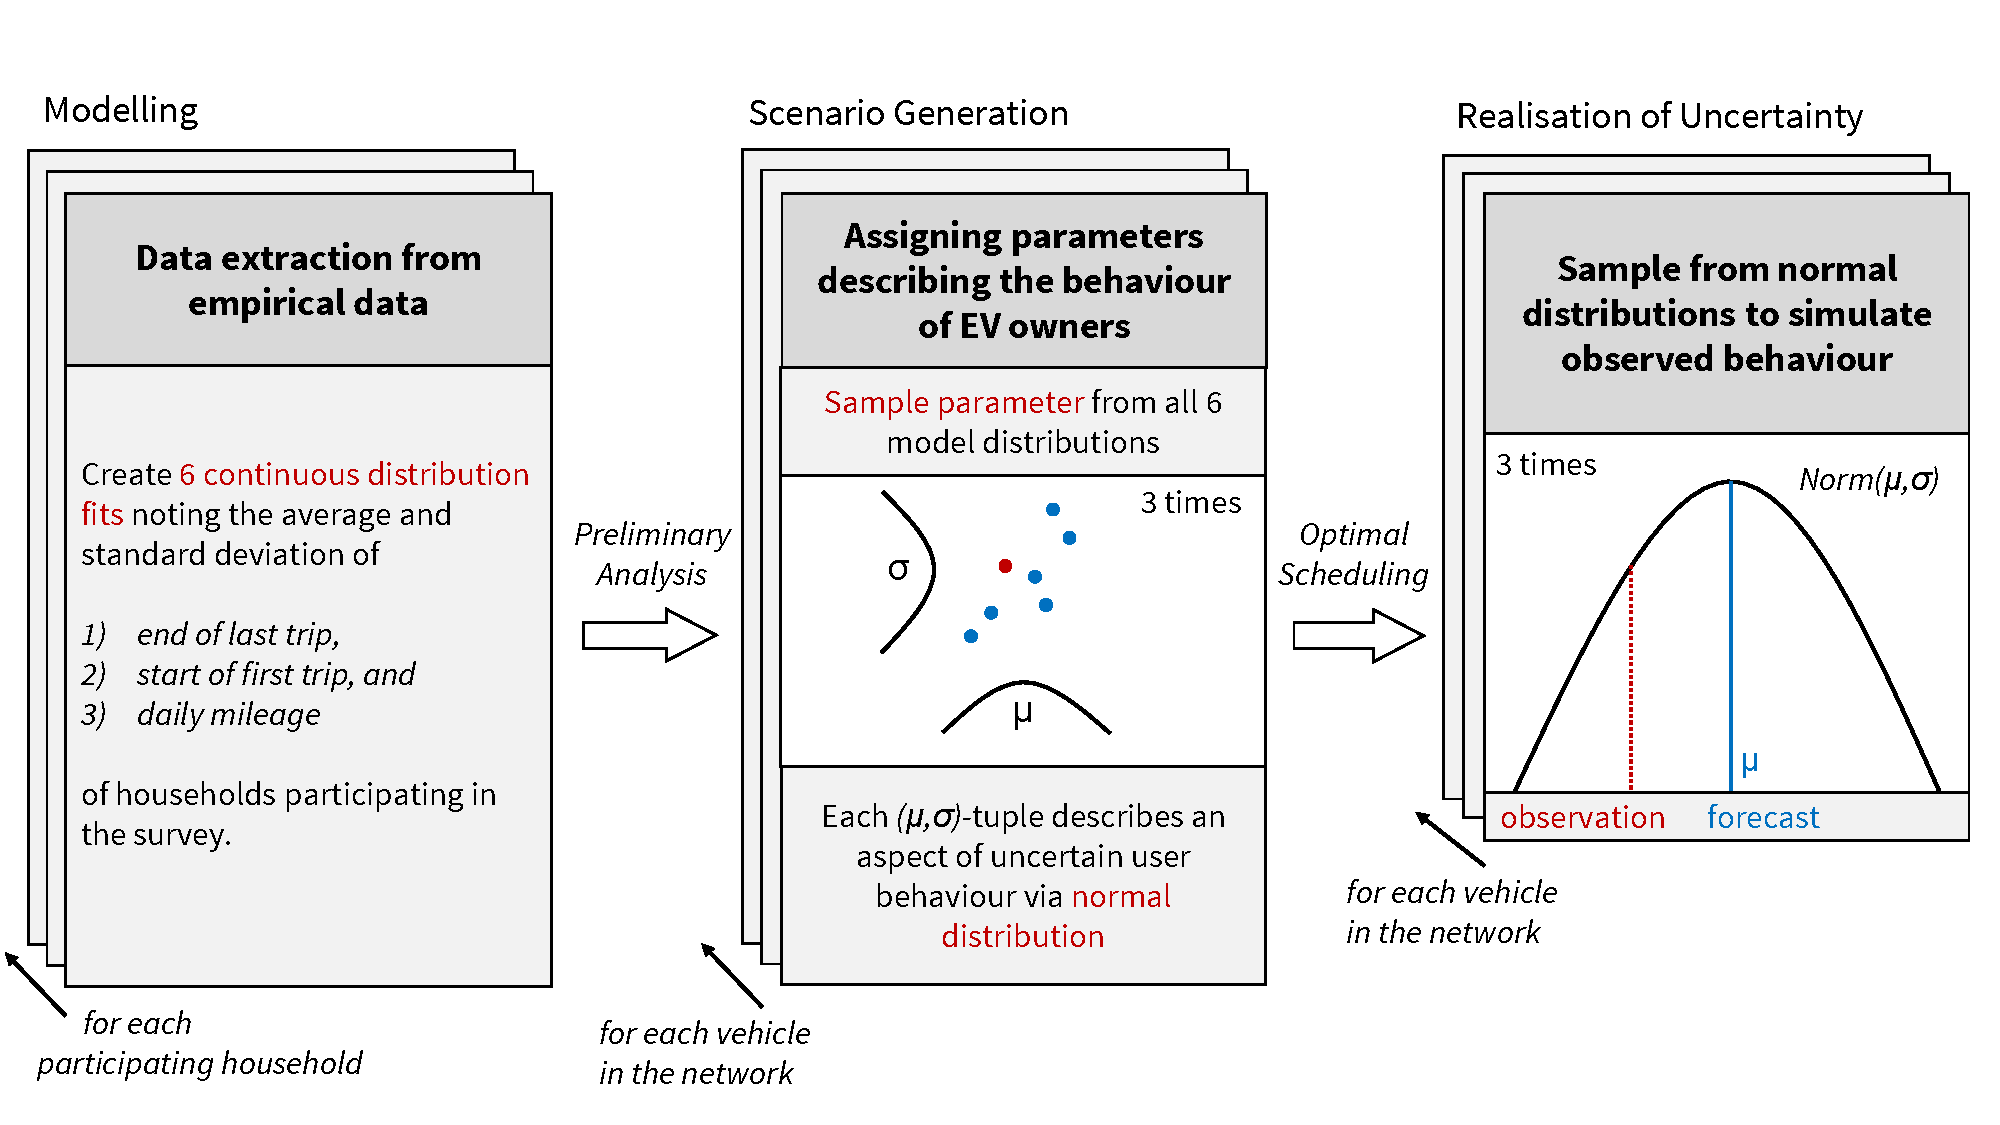
\includegraphics[width=.9\textwidth,trim={0cm 0.5cm 0cm 0.8cm},clip]{figures/mobility/flow}
	\caption{Illustration of travel pattern model derivation and application}
	\label{fig:flow}
\end{figure}

\subsection{Data Source and Extraction}

% mention possible data sources and assumptions made

Due to the limited market penetration of electric vehicles to date, appropriate data sets on the mobility of EV owners are sparse. To circumvent this problem, the developed model is based on empirical driving profiles of internal combustion vehicles. Thereby, it is assumed that a majority of travel patterns will not be influenced by a transition from conventional vehicles to electric vehicles in private transport, although this is not unquestioned \cite{Schauble2017}. Nonetheless, this approach is commonly applied in research on EV charging modelling and is deemed particularly reasonable for inferring charging requirements \cite{Schuller2013,Flath2013, Wang2017, Daina2017,Pasaoglu2013,Wu2010b}. 

To model the behaviour of UK customers, mobility data was obtained from the UK National Travel Survey \cite{NTS2017}. This extensive survey is updated annually and contains a multitude of disaggregated data about means, demographics and behaviour of personal travel based on record diaries from 2002 to 2015. Given the amount of data provided, only a sufficiently large extract of trip data of the most recent 4,000 households with a total of 30,000 trips by car logged was used. 

% simplifications regarding clustering and weekday differentiation & neglected differentiations

As trip data is quite heterogeneous regarding trip purposes, weekdays and demographic groups, clustering as undertaken in related work appears sensible and will result in a differentiated representation of the reality \cite{Schuller2013, Acha2012}. For the sake of exposition, the developed mobility model focusses on weekdays and makes no differentiation between demographic groups or trip purposes. Although this simplification lacks the sophistication achieved by clustering, it will comprise the most challenging days for EV charging and could easily be remedied by mere repetition of analysis. Hence, the trip data is filtered only to extract trips by cars on weekdays. Moreover, to avoid too small sample sizes households with less than three days logged in the record books are excluded. Subsequently, the data set was examined further to find measures for the average $\mu$ and standard deviation $\sigma$ of daily mileage, arrival and departure times of individual households. This provides an alternative to developing a stochastic mobility model based on Markov chains or agent-based methods as elaborated in i.a.\ \cite{Soares2011, Acha2012,Galus2011,Hu2016}. However, involved uncertainty has only been analysed for a limited number of studies \cite{Wang2017,Zhang2014}.

% describe method of size reduction and pre-calculations on data set 

\subsubsection*{Arrival and Departure Times}

In practice, an electric vehicle may arrive and depart at multiple locations and times of the day. But, because the assumed scenario is confined to scheduling for charging at home overnight, the ambiguity of the terms arrival and departure time can be resolved \cite{Dallinger2010a}. While the arrival time refers to arrival at home after the last trip of the day, the departure time refers to the departure from home just before the first journey of the next day. For each household, the average and standard deviation of these arrival and departure times among the logged days are determined and compiled to two sets of ($\mu$,$\sigma$)-tuples characterising the required information about a household's EV availability.

\subsubsection*{Daily Mileage}

Daily trip distances in the data set are obtained from the sum of all individual trips for each household and logged day. Given the range of modelled electric vehicles as specified through the battery capacity and consumption in \Autoref{sec:ev}, infeasible trip distances outwith the EV range of 120 miles are discarded. Then, similar to the arrival and departure times, the values for the daily mileage are recorded as a set of ($\mu$,$\sigma$)-tuples describing a car's typical driving distance.

\subsection{Analysis of Empirical Data}

% qualitatively analyse histograms of empirical data

Histograms of the acquired ($\mu$,$\sigma$)-tuples are depicted in \Autoref{fig:mobilityfits}, emphasising the heterogeneity of both average and variance values of parameters among participating households. In an average household, the first trip by car occurs at 10:30 am while the last trip ends 16:45 pm. Throughout the day this household has travelled 22 miles or 35 km. Normally, an average household deviates between 2 and 2.5 hours from its average departure/arrival times and 15 miles or 24 km from its expected daily mileage. These values are surprisingly high and exceed expectations on the uncertainty involved. A comprehensive list of shape parameters such as skewness and kurtosis are compiled in \Autoref{tab:shapeparams}.

\begin{figure}[tp]
	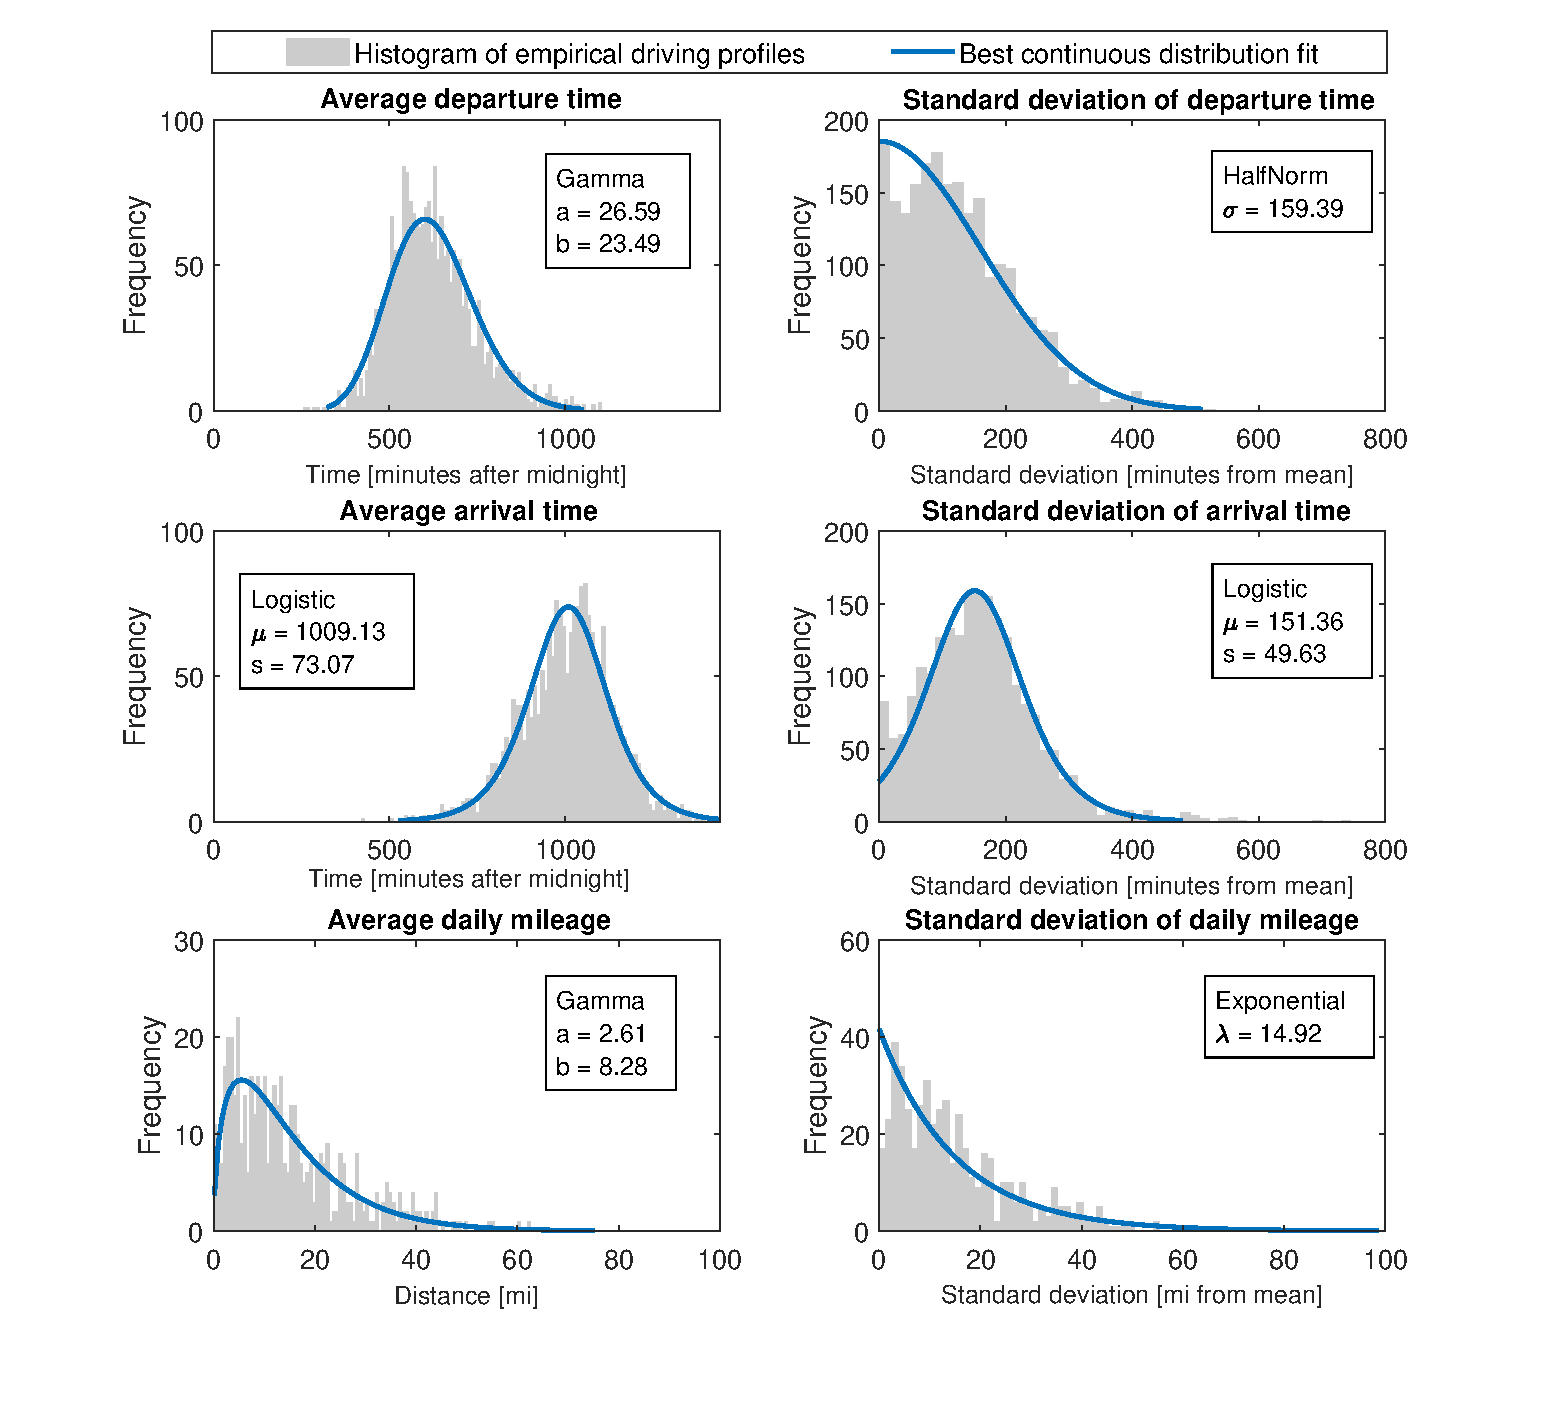
\includegraphics[width=\textwidth,trim={1.5cm 1.2cm 2cm 0cm},clip]{figures/mobility/mobilityfits.eps}
	\caption{Marginal distribution fits of ($\mu$,$\sigma$)-tuples of daily mileage, arrival and departure times}
	\label{fig:mobilityfits}
\end{figure}

% describe parameters of marginal distribution fits

\Autoref{fig:mobilityfits} moreover includes continuous distributions fitted to the empirical driving profiles. Extracting the relevant statistical information from the travel survey to build a generic EV user model without massive data sets facilitates its scalability, reproducibility and calibration. Approximating driving distances by Gamma distributions has been applied and validated in research papers \cite{Flath2013, Plotz2017}.

The distribution for each parameter is chosen based on the Akaike information criterion (AIC) which compares the relative quality of models for a given data set. This approach results in four types of distributions describing the six random variables of the mobility behaviour model, the parameters to which are complemented in \Autoref{fig:mobilityfits}.

Average departure time and daily mileage are described by a Gamma distribution denoted by the probability density function

\begin{equation}
f_{\mathrm{Gamma}}(x;a,\theta) = \begin{cases}
\frac{ \theta^{-a}}{\Gamma(a)}x^{a-1} e^{- \frac{x}{\theta}} & x \geq 0 \\
0 & x < 0
\end{cases} \quad \text{ for } a, \theta > 0
\end{equation}

The average and standard deviation of arrival times are approximated by a truncated logistic distribution with the probability density function

\begin{equation}
f_{\mathrm{Logistic}}(x; \mu,s) = \begin{cases}
\frac{e^{-\frac{x-\mu}{s}}} {s\left(1+e^{-\frac{x-\mu}{s}}\right)^2} & x \geq 0 \\
0 & x < 0
\end{cases}
\end{equation}

The standard deviation of departure times follows a half normal distribution with the probability 

\begin{equation}
f_{\mathrm{HalfNorm}}(x; \sigma) = \left|\frac{\sqrt{2}}{\sigma\sqrt{\pi}} \,\cdot\, e^{-\frac{x^2}{2\sigma^2} } \right|
\end{equation}

Finally, the standard deviation of daily mileage shows exponential characteristics with the probability density function

\begin{equation}
f_{\mathrm{Expo}}(x;\lambda) = \begin{cases}
\lambda e^{-\lambda x} & x \ge 0, \\
0 & x < 0.
\end{cases}
\end{equation}

% discuss quality and validity of marginal distribution fits

The accuracy of the fits could be confirmed neither by a Kolmogorov-Smirnov nor a $\chi^2$ statistic. The major obstacle is the heterogeneity of profiles \cite{Flath2013}. Partly, this is also not achieved due to the spikes resulting from rounding times in the log book and the truncation of the distributions to the interval $[0,\infty)$. Instead, the shape parameters of the distribution fits are compared to the underlying empirical data in \Autoref{tab:shapeparams}. While the distribution fits excel at approximating mean and variance, they tend to underestimate skewness and kurtosis.

% Please add the following required packages to your document preamble:
% \usepackage{booktabs}
% \usepackage{multirow}
\begin{table}[tp]
	\centering
	
	%\small
	\resizebox{\textwidth}{!} {%
	\begin{tabular}{@{}lllllll@{}}
		
		\toprule
		\textbf{}                                & \textbf{}                 & \textbf{}       & \textbf{Mean $\mu$} & \textbf{Variance $\sigma^2$} & \textbf{Skewness $\gamma_1$} & \textbf{Kurtosis $\gamma_2$} \\ \midrule
		\multirow{4}{*}{\textbf{Arrival time}}   & \multirow{2}{*}{$\mu$}    & empirical       & 1005.40             & 16907                        & -0.31                       & 3.48                       \\
		&                           & logistic fit    & 1009.13             & 17565                        & 0                            & 1.20                          \\
		& \multirow{2}{*}{$\sigma$} & empirical       & 156.44              & 8312                         & 1.007                        & 5.72                        \\
		&                           & logisitc fit    & 151.36              & 8105                         & 0                            & 1.20                          \\ \midrule
		\multirow{4}{*}{\textbf{Departure time}} & \multirow{2}{*}{$\mu$}    & empirical       & 624.56              & 15231                        & 0.723                        & 3.89                        \\
		&                           & gamma fit       & 624.55              & 15945                        & 0.194                        & 0.23                        \\
		& \multirow{2}{*}{$\sigma$} & empirical       & 129.76              & 8571                         & 0.994                        & 4.83                        \\
		&                           & halfnormal fit  & 127.18              & 9232                         & 0.995                        & 0.87                       \\ \midrule
		\multirow{4}{*}{\textbf{Daily mileage}}  & \multirow{2}{*}{$\mu$}    & empirical       & 21.63               & 192.83                       & 1.602                        & 7.65                        \\
		&                           & gamma fit       & 21.63               & 178.98                       & 0.619                        & 2.30                        \\
		& \multirow{2}{*}{$\sigma$} & empirical       & 14.92             & 140.35                     & 1.173                       & 4.07                       \\
		&                           & exponential fit & 14.92             & 140.35                     & 2                            & 6                            \\ \bottomrule
	\end{tabular}
	}
	\caption{Shape parameters of empirical trip data and distribution fits}
	\label{tab:shapeparams}
\end{table}

% highlight multivariate nature of sigma mu pairs --> describe method of generating multivariate distributions given the two marginal distributions of sigma and mu

So far only the marginal distributions of the ($\mu$,$\sigma$)-tuples have been addressed. However, it is far from obvious that for example the average daily mileage and its standard deviation are uncorrelated. In fact, these feature the strongest correlation coefficient\footnote{Sample Pearson correlation coefficient $$r =\frac{\sum ^n _{i=1}(x_i - \bar{x})(y_i - \bar{y})}{\sqrt{\sum ^n _{i=1}(x_i - \bar{x})^2} \sqrt{\sum ^n _{i=1}(y_i - \bar{y})^2}}$$} $r=0.681$. With $r=0.355$ the ($\mu$,$\sigma$)-tuples of departure times show a moderate positive correlation, while arrival times only exhibit a weak negative correlation with $r=-0.142$ and will therefore be regarded as independent random variables. \Autoref{fig:simmil} illustrates the correlations and underlines the importance for the model to handle the ($\mu$,$\sigma$)-tuples as multivariate random variables with their marginal distributions given by the respective distributions for $\mu$ and $\sigma$.

A simple way to realise a multivariate random variable with various marginal distributions in Scipy or MATLAB is to initially generate a sample from a multivariate standard normal distribution $\mathcal{N}_2(\bm{\mu},\bm{\rho})$ specified by its means $\bm{\mu} = (0,0)^T$ and the empirical 2-by-2 matrix of correlation coefficients $\bm{\rho}$ \cite{Waldmann2016}. Then each of the two elements is transformed to match the desired marginal distribution in two steps via an intermediary transformation to the uniform distribution $\mathcal{U}(0,1)$.

Let the random tuple $(z_1,z_2)$ be a realisation of the random variable $Z \sim \mathcal{N}_2(\bm{\mu},\bm{\rho})$ and let $F_{\mathcal{U}(0,1)}$ denote the cumulative distribution function (CDF) of $\mathcal{U}(0,1)$. Moreover, let $F_{\mathcal{M}_1}$ and $F_{\mathcal{M}_2}$ represent the CDFs of the two marginal distributions belonging to the desired multivariate distribution $\mathcal{M}$. Then, if 

\begin{equation}
	 \begin{pmatrix}
	 x_1 \\
	 x_2 
	 \end{pmatrix}^T = \begin{pmatrix}
	 F^{-1}_{\mathcal{M}_1}\left[\,F_{\mathcal{U}(0,1)}(z_1)\,\right] \\
	 F^{-1}_{\mathcal{M}_2}\left[\,F_{\mathcal{U}(0,1)}(z_2)\,\right]
	 \end{pmatrix}^T
\end{equation}

the tuple $(x_1,x_2)$ is regarded as a realisation of the random variable $X \sim \mathcal{M}$. 

\begin{figure}[tp]
	\centering
	\subfloat{
		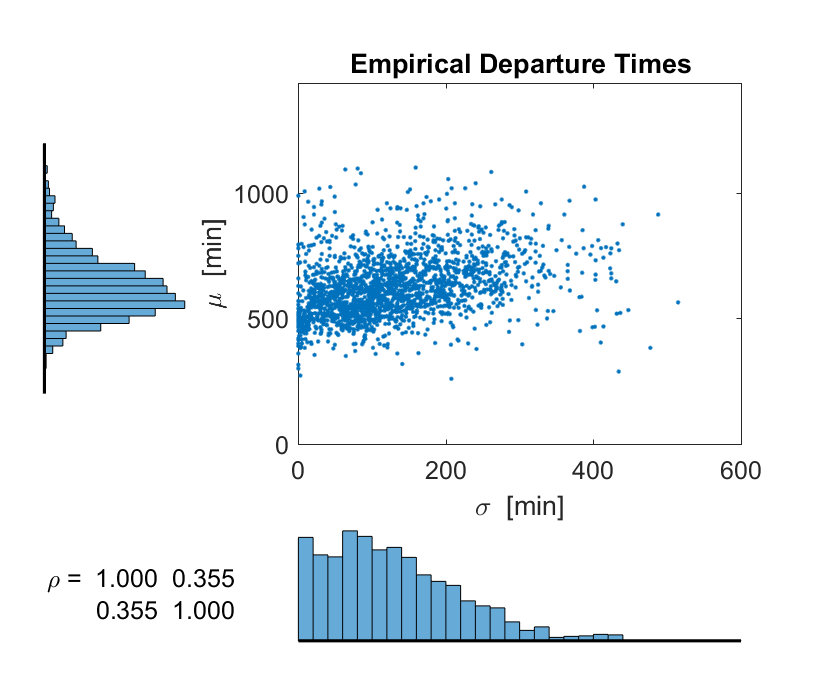
\includegraphics[width=0.48\textwidth,trim={0.4cm 0.4cm 0.4cm 0.4cm}, clip]{figures/mobility/emp_dep.eps}
	}
	\subfloat{
		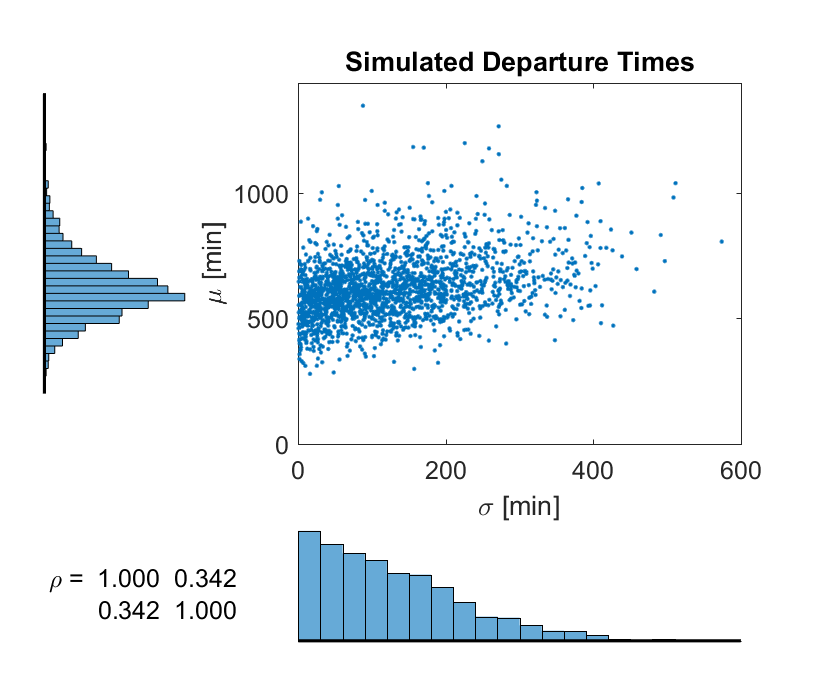
\includegraphics[width=0.48\textwidth,trim={0.4cm 0.4cm 0.4cm 0.4cm}, clip]{figures/mobility/sim_dep.eps}
	}
	\hfill
	\subfloat{
		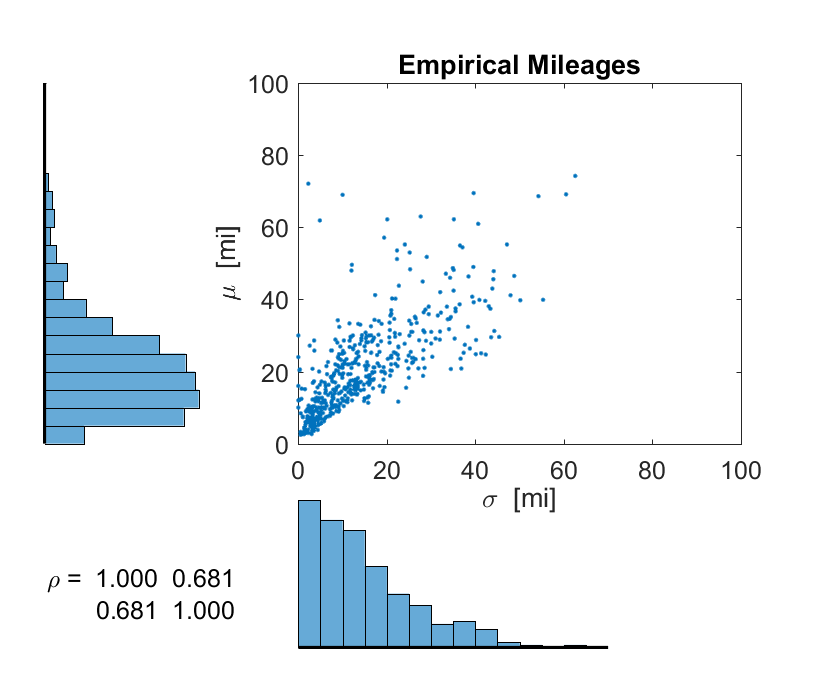
\includegraphics[width=0.48\textwidth,trim={0.4cm 0.4cm 0.4cm 0.4cm}, clip]{figures/mobility/emp_mil.eps}
	}
	\subfloat{
		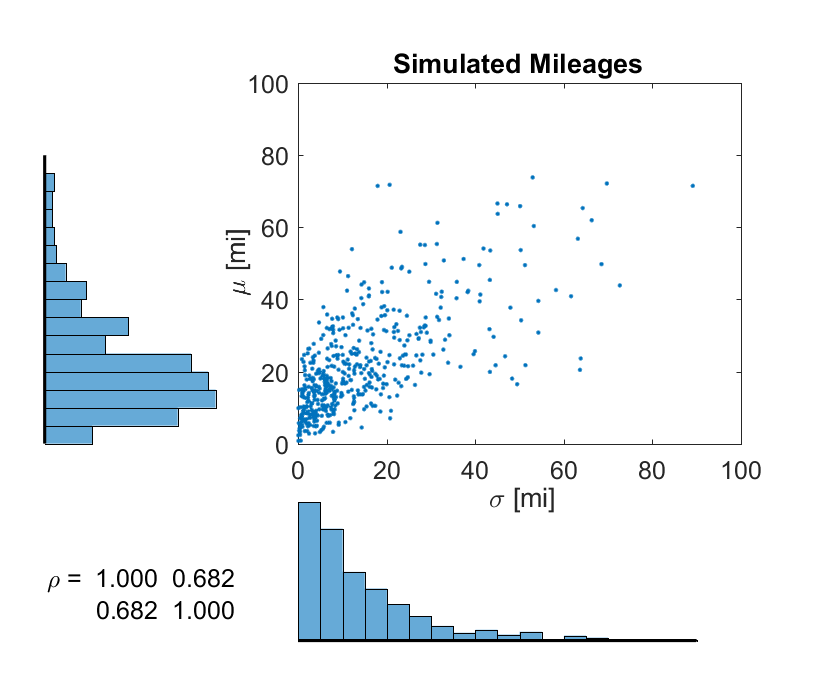
\includegraphics[width=0.48\textwidth,trim={0.4cm 0.4cm 0.4cm 0.4cm}, clip]{figures/mobility/sim_mil.eps}	
	}
	\caption{Correlation of ($\mu$,$\sigma$)-tuples in empirical and simulated driving patterns}
	\label{fig:simmil}
\end{figure}

\newpage
The validity of this approach is investigated by simulating a set of tuples with the size of the empirical data set as presented in the right column of \Autoref{fig:simmil}. The resemblance of empirical and simulated profiles is distinct and supported by similar correlation coefficients of $r=0.682$ for simulated mileages and $r=0.342$ for simulated departure times.

\subsection{Modelling User Behaviour}
\label{sec:mub}

Many studies use empirical or fitted distributions of daily mileage, arrival and departure times for a stochastic scenario generation \cite{Budenbender,Flath2013, Schuller2013, Wu2013,Contreras-Ocana2016, Guo2016, Peppanen2014, Li2014, Salah2016, Richstein2012, Garttner2016c}. Typically, after randomly assigning these parameters to households, they are regarded immutable. A representation of uncertainty involved for each user based on empirical data is, however, less widespread. The acquired knowledge from the preceding sections enables both, stochastic scenario generation and representation of operational uncertainty.

\subsubsection*{Scenario Generation}

The parameters shaping the mobility behaviour of EV owners are generated through realisations of their respective distribution functions and iteratively assigned to households in the test network. The small sample size of days at each household of the survey on which the analysis is based -- peaking at 14 days -- permits no distribution assumption other than the normal distribution $\mathcal{N}(\mu,\sigma)$ for the troika of $(\mu,\sigma)$-tuples defining daily mileage $\tilde{\delta}_{mil}$, arrival time $\tilde{\tau}_{arr}$ and departure time $\tilde{\tau}_{dep}$:

% maximum likelihood: by default forecast is mu as expectation value of normal distribution

\begin{subequations}
	\begin{equation}
		\tilde{\delta}_{mil} \sim \mathcal{N}(\mu_{mil},\sigma_{mil}) \qquad \text{and} \qquad \hat{\delta}_{mil} = \mathbb{E}[\tilde{\delta}_{mil}]= \mu_{mil}
	\end{equation}
	\begin{equation}
		\tilde{\tau}_{arr} \sim \mathcal{N}(\mu_{arr},\sigma_{arr}) \qquad \text{and} \qquad \hat{\tau}_{arr} = \mathbb{E}[\tilde{\tau}_{arr}] = \mu_{arr}
	\end{equation}
	\begin{equation}
		\tilde{\tau}_{dep} \sim \mathcal{N}(\mu_{dep},\sigma_{dep}) \qquad \text{and} \qquad \hat{\tau}_{dep} = \mathbb{E}[\tilde{\tau}_{dep}] = \mu_{dep}
	\end{equation}
\end{subequations}

Simulation under uncertainty will treat $\hat{\delta}_{mil}$, $\hat{\tau}_{arr}$, and $\hat{\tau}_{dep}$ as forecasts and use a realisation of the random variables $\tilde{\delta}_{mil}$, $\tilde{\tau}_{arr}$, and $\tilde{\tau}_{dep}$ to emulate a deviation from predicted parameters.


\subsubsection*{EV Charging Demand}

% tranlate daily mileage to energy consumption / charging demand

Due to the one-to-one correspondence of daily mileage and EV battery discharge linked by the consumption $\zeta = 0.17$ kWh/km and the conversion factor 1.609 km/mi, the battery state of charge upon arrival $\tilde{B}^{arr}$ also follows a normal distribution \cite{Flath2013}. Assuming a full battery at the beginning of the day with a charging level $B_{max} = 30$ kWh and the user does not charge anywhere but at home overnight

\begin{equation}
	\tilde{B}^{arr} = B_{max} - 1.609 \cdot \zeta \cdot \tilde{\delta}_{mil} \qquad \text{and} \qquad \hat{B}^{arr} = B_{max} - 1.609 \cdot \zeta \cdot \hat{\delta}_{mil}.
\end{equation}

If no vehicle belongs to a household, $\tilde{B}^{arr} = \hat{B}^{arr} = {B}^{arr} = B_{max} = 30$ kWh.

\subsubsection*{EV Availability}

The availability of an electric vehicle $\tilde{\alpha}^{EV}\in \mathbb{B}^T$ throughout the optimisation horizon $T=96$ is determined by $\tilde{\tau}_{arr}$, $\tilde{\tau}_{dep}$ and their conversion to time slots $t\in T$:

\begin{equation}
	\tilde{\alpha}^{EV}_t =
	\begin{cases}
	1 & \text{if } \left\lfloor \max \left(0,\; \frac{\tilde{\tau}_{arr}\,-\,\tau_{init}}{\Delta t \cdot 60}\right) \right\rfloor \leq t < \left\lfloor \min \left(T,\; T + \frac{\tilde{\tau}_{dep}\,-\,\tau_{init}}{\Delta t \cdot 60}\right) \right\rfloor\\
	0 & \text{else} 
	\end{cases} \qquad \forall t \in T
\end{equation}

where $\tau_{init} = 660$ min is the time of the day in minutes after midnight at which the optimisation routine starts and $\Delta t$ denotes the granularity. Note that if $\tilde{\tau}_{arr}>\tilde{\tau}_{dep}$ the electric vehicle did not return that night and will not be available for charging at all. The expected availability $\hat{\alpha}^{EV}$ is defined analogously. If no vehicle belongs to a household, $\tilde{\alpha}^{EV}_t = \hat{\alpha}^{EV}_t = {\alpha}^{EV}_t = 0$.

% availability: build availability probabilities 

The probability $\mathbb{P}_t(\alpha^{EV}=1)$ that a vehicle is available in time slot $t$ is calculated using the CDF of the tabulated standard normal distribution $\Phi$ involving the conversion of time slots $t\in T$ to minutes after midnight.

\begin{equation}
\begin{split}
	\mathbb{P}_t\left(\alpha^{EV}=1\right) = \min &\overbrace{\left\{\Phi\left(\frac{ (t \cdot \Delta t \cdot 60 + \tau_{init})-\mu_{arr}}{\sigma_{arr}}\right)\right.}^{\text{probability that vehicle has arrived}},\;\\
& \:\:\,\underbrace{\left.\Phi\left(\frac{ (t \cdot \Delta t \cdot 60 + \tau_{init} - T\cdot \Delta t \cdot 60)-\mu_{dep}}{\sigma_{dep}}\right) \;\right\}}_{\text{probability that vehicle has departed}} \qquad \forall t \in T
\end{split}
\end{equation}

The obtained time series is expedient for the mitigation of availability uncertainty in \mbox{\Autoref{sec:av_unc}}. Exemplary availability probability curves, as well as an average availability probability curve of 55 vehicles, are illustrated in \Autoref{fig:ex_av}. Clearly, the availability of an EV is most likely in the early morning hours and as required reduces towards noon.

% something about average parking duration... 17.5 hours seems so long!

\begin{figure}[b]
	\centering
	\subfloat{
		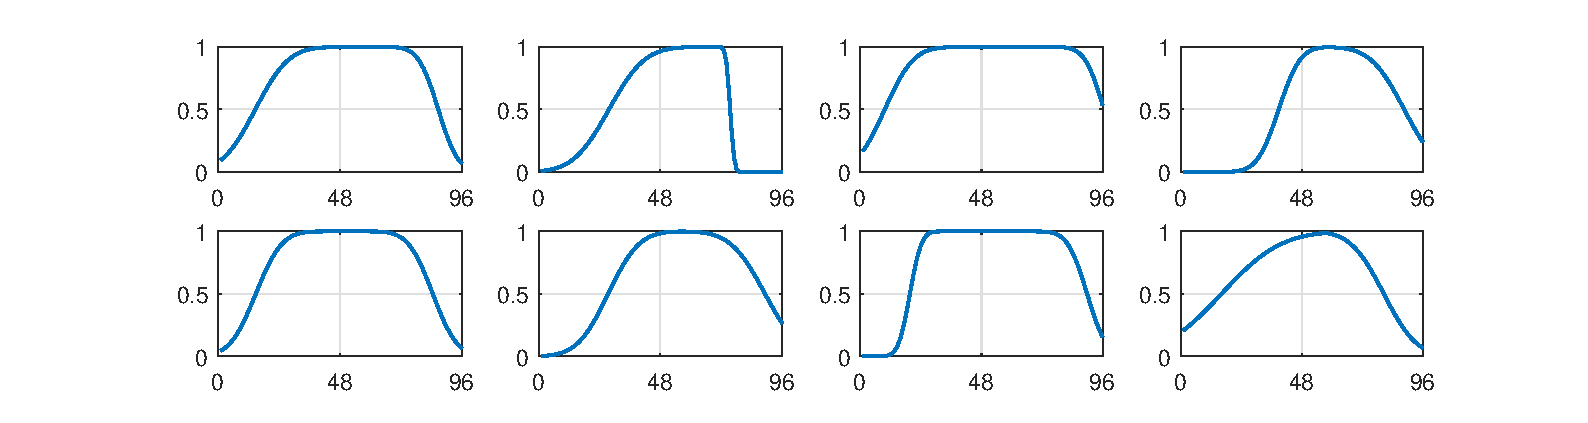
\includegraphics[width=\textwidth,trim={1.5cm 0cm 1.5cm 0cm}, clip]{figures/availability/ex_av.eps}
	
	}
	\vspace{-.5cm}
	\hfill
	\subfloat{
		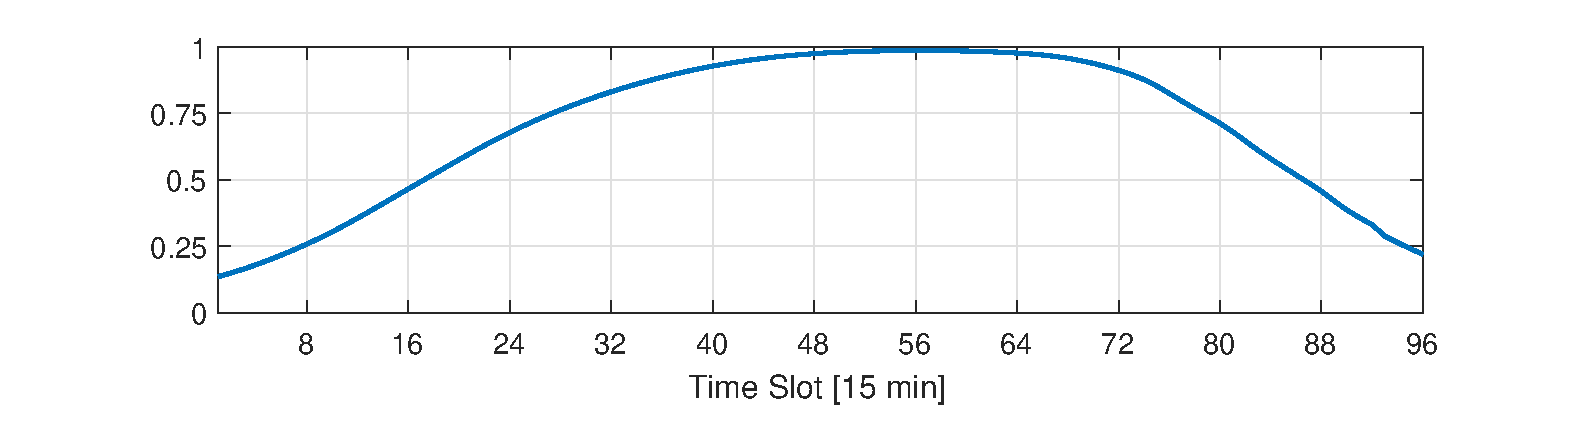
\includegraphics[width=\textwidth,trim={1.5cm 0cm 1.5cm 0cm}, clip]{figures/availability/av_av.eps}
	}
	\caption{Illustration of availability probabilities on an individual (top) or aggregate level (bottom)}
	\label{fig:ex_av}
\end{figure}

\section{Electricity Prices}
\label{sec:ep}

% dynamic tariffs

Dynamically adjusted, time-varying electricity prices as an incentive for stimulating demand-side management are uncommon at the consumer level. Most energy providers offer their customers single or dual rate tariffs, where the latter normally offers a lower price during off-peak periods at night in exchange for a higher price during on-peak hours. 

% support

Support for the integration of intermittent generation by DR or DSM is assumed to be incentivised via wholesale electricity prices. Due to the merit-order effect, the wholesale electricity prices may be used as a proxy for the network state \cite{Kirschen2004}. While low prices indicate low demand or a high share of renewable energy generation and call for an increase in demand, high prices signal peak demand coupled with low renewable generation and urge for a deferral of power demand.

Consequently, the rationale for scheduling approaches seeking to relief network strain and expedite the integration of renewables is to shift deferrable loads to periods with low prices.

\subsection{Modelling}

% data source and illustration, justify choice

To reflect UK power market characteristics, the model for price time series is based on the reference price data (RPD) indices for the EPEX SPOT UK\footnote{formerly APX Power UK / UKPX; first independent power exchange in the UK operating since 2001} energy exchange market, providing a volume-weighted reference price for each half-hourly settlement period. A pool of the 1,000 most recent price profiles is stored from which the stochastic scenario generation picks randomly. \Autoref{fig:var_price} illustrates the diversity of stored price profiles and underlines the tendencies for lower prices at night and price peak during peak demand. Noteworthily, at night outliers below the median dominate while early evening hours exhibit significant outliers above the median concerning both, frequency and magnitude.

\begin{figure}[tp]
	\centering
	\subfloat[Boxplots of stored price profiles]{
		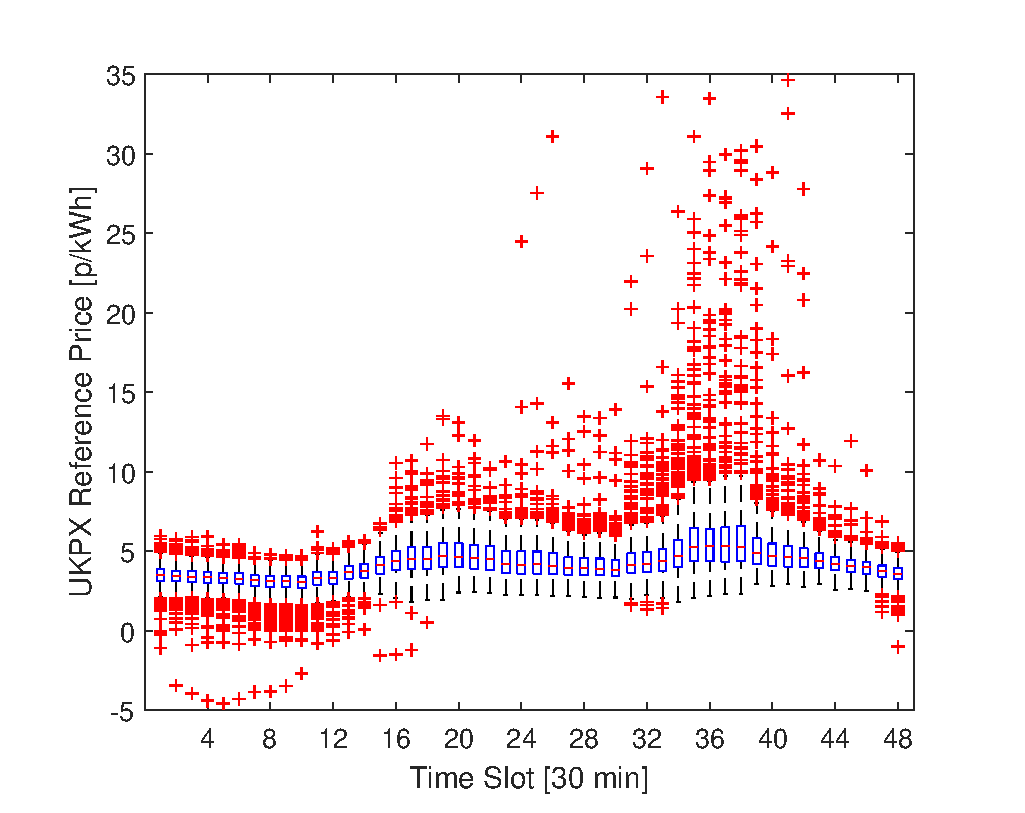
\includegraphics[width=0.48\textwidth]{figures/prices/boxplots_prices.eps}
		\label{fig:pricebox}
	}
	\hfill
	\subfloat[Exemplary price time series (p/kWh)]{
		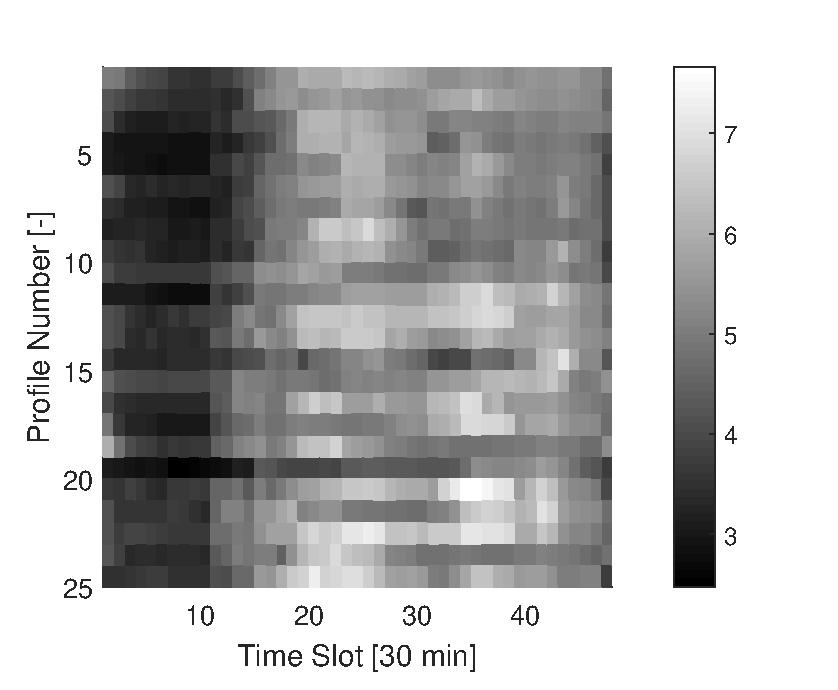
\includegraphics[width=0.48\textwidth]{figures/prices/exemplary_prices.eps}
		\label{fig:exampleprice}
	}
	\caption{Illustration of the variety in price profiles}
	\label{fig:var_price}
\end{figure}

% accessibility - adaptations

In order to unfold the control effect of time-variable pricing, accessibility to customers is essential. This is provided by the aggregator participating in the wholesale market on behalf of the economic interest of its customers. The EPEX SPOT market, however, neither includes license and transmission fees nor taxes, which the aggregator undoubtedly would be charged for selling electricity and pass these costs on. Such charges and fees are mostly constant. The problem with constant charges and fees is that they distort the characteristics of the market price and reduce the signal function for DSM \cite{Jansen2015}. The price of generation and supply is only a fraction of the final electricity price. While static surcharges preserve the ranking of the original price signal and are therefore inconsequential for price-based scheduling approaches, it limits the potential savings of charging coordination. One approach to turn the premiums from a barrier into a driver of demand-side management is to couple the grid charges to the flexible price signal using a multiplicative factor; equivalent to variable fees or taxes. This way the absolute difference of prices is increased and the price signal is amplified. Hence, control agents are further nudged to act market-compliantly through corporate or government incentives \cite{Jansen2015}. 

To simulate the price signal with both variable and static surcharges that on average corresponds to the average retail electricity price of UK single-rate tariffs, the expected price profile is spread around its mean

\begin{equation}
\bar{\pi} = \frac{1}{48}\sum_{t=1}^{48}\hat{\pi}^{EPEX}_t
\end{equation}

by the factor $s=5$ and a constant price addition of $q = 14$ p/kWh is added

\begin{equation}
\hat{\pi}_t = \left(\hat{\pi}^{EPEX}_t-\bar{\pi}\right) \cdot s + \bar{\pi} + q \qquad \forall t \in \{1,\dots,48\}
\end{equation}

to yield the price profile $\hat{\pi}= \left(\hat{\pi}_1,\dots,\hat{\pi}_{48}\right)\in \mathbb{R}^{48}$.

% market power of EV aggregators

\newpage
For simplicity, the influence of additional EV loads on electricity prices is disregarded, and aggregators are not significant enough to exert any market power; i.e.\ all aggregators act as price-takers on the wholesale market \cite{Balram2014, GonzalezVaya2015, Hu2016, Koch2012, Rotering2011}. Moreover, to add variety to the model, the price profiles may be used as a representation of day-ahead or intraday spot market prices depending on the chosen scenario.

% locational marginal prices?

% technical adaptation

To match the number of time intervals of the optimisation routine, the price time series $\hat{\pi}$ is expanded such that for a 24-hour optimisation at 15-minute intervals the price profile becomes

\begin{equation}
\hat{\pi}' = \left(\hat{\pi}_1,\hat{\pi}_1,\dots,\hat{\pi}_{48},\hat{\pi}_{48}\right) \in \mathbb{R}^{96}
\end{equation}

This eschews interpolation and preserves the half-hourly interval of price changes.

\subsection{Uncertainty Representation}
\label{sec:pr_unc}

% general model

The uncertain price profile $\tilde{\pi}\in \mathbb{R}^{48}$ is modelled by a sequence of factors $\kappa \in \mathbb{R}^{48}$ describing the severity of price uncertainty of a time slot as the standard deviation of the forecasted prices $\hat{\pi}$ and a sequence of Gaussian noise $\xi\in \mathbb{R}^{48}$ where $\xi_t\sim \mathcal{N}(0,1)$, such that

\begin{equation}
\tilde{\pi}_t = \hat{\pi}_t + \kappa_t \cdot \xi_t
\end{equation}

and $\tilde{\pi}_t\sim \mathcal{N}\left(\hat{\pi}_t, \kappa_t\right)$. Because the price deviations are likely to be serially correlated in time \cite{Wu2010}, independent Gaussian white noise is unsuitable for the error sequence $\xi$. So-called red noise considers the lag-1 autocorrelation $r$ between two successive elements, and better reflects the dependence of forecast errors in consecutive time steps \cite{Bretherton2014}. A sequence of red noise is generated from a $\mathcal{N}(0,1)$ white noise sequence $\omega\in \mathbb{R}^{48}$ by setting

\begin{subequations}
	\begin{equation}
	\xi_1 = \omega_1
	\end{equation}
	\begin{equation}
	\xi_{t+1} = r\cdot \xi_t + \sqrt{1-r^2} \cdot \omega_{t+1} \qquad \text{for } t > 1.
	\end{equation}
\end{subequations}

Thereby, a strong lag-1 correlation coefficient $r=0.7$ of $\xi_{t}$ and $\xi_{t+1}$ is achieved while maintaining that $\xi_{t}$ follows $\mathcal{N}(0,1)$ \cite{Bretherton2014}. 

% kappa
\newpage
Using the sequence $\kappa$ to define the standard deviation of uncertainty relies on the assumption that a statement not only about the range but also about probability distribution of errors can be obtained from price forecasting mechanisms \cite{Niimura2006,Weron2014a}. For the model, the factor $\kappa_t$ consists of three distinct terms:

\begin{equation}
\kappa_t \;=\; 0.5 \;+\; \frac{|\xi_t|}{4} \;+\; \frac{\left|\hat{\pi}_t-(\bar{\pi}+q)\right|}{\max\left\{\,\left|\hat{\pi}_t-(\bar{\pi}+q)\right| ;\; t \in \{1,\dots,48\}\,\right\} }
\end{equation}

The first summand is the minimum standard deviation of any forecast, the second summand introduces a minor red noise error term to distort the ranking of the simulated price profile compared to its projections, and the third summand normalises the deviation of the price forecast from its mean. This reasonably assumes that price extremes tend to be burdened with particular uncertainty compared to prices closer to the average due to peak demand in one case and an expected high share of intermittent generation in the other. The term weightings were chosen arbitrarily and may be adapted to suit different assumptions about price uncertainty. Approximating the maximum of $\xi_t$ by three standard deviations and noting that the third term lies in the interval [0,1], this configuration maintains $\kappa_t$ in a range between 0.5 and 2.25 p/kWh, which results in reasonable error bands as illustrated in \Autoref{fig:priceuncertainty} \cite{OConnell2014}.
 
\begin{figure}[tp] % TODO update!
	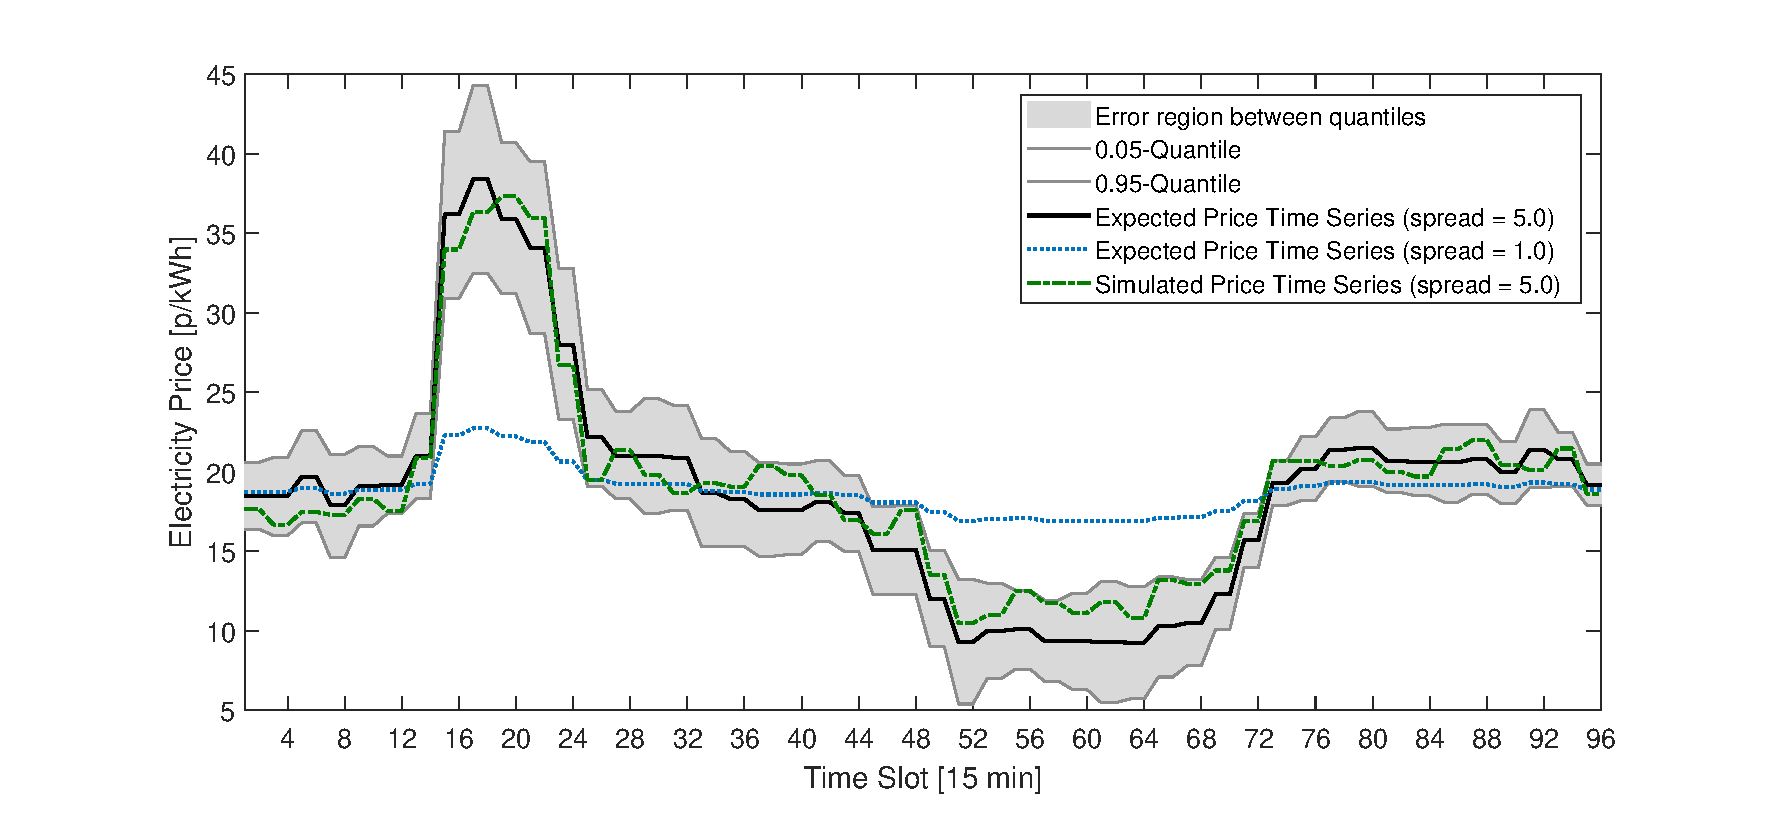
\includegraphics[width=\textwidth,trim={2cm 0cm 2cm 0cm},clip]{figures/prices/price_uncertainty.eps}
	\caption{Exemplary illustration of uncertainty in price time series}
	\label{fig:priceuncertainty}
\end{figure}
\chapter{Optimisation under Uncertainty}
\label{sec:opt}

This chapter is dedicated to introducing applied optimisation and modification concepts. It commences with the mathematical problem formulation in \Autoref{sec:pf} building on the parameters presented in \Autoref{sec:model}, where objectives and constraints are categorised and complemented with an explanation of their purpose. Furthermore, a method for linear power flow approximation to enable solutions obtained from quick linear programming. Subsequently reference charging approaches are introduced in \Autoref{sec:rc} against which coordinating scheduling algorithms are held as a benchmark. These are presented and discussed in \Autoref{sec:chargecoordination} before addressing various methods of uncertainty mitigation in \Autoref{sec:uncmitigation}.

\section{Problem Formulation}
\label{sec:pf}

Following a time discretization to avoid formal representations by differential equations, constant charging powers within each time slot are assumed. Across time slots $\Delta t = 0.25$ hours, the charging rates are continuous and are denoted by the matrix of decision variables  $P^{EV}\in \mathbb{R}^{K\times T}$.

\subsection{Objectives}

The objective function is designed to find a set of schedules $P^{EV}$ which minimise the costs of charging a pool of electric vehicles in discrete time steps $\Delta t$. Primarily, it is a customer-focused objective providing an incentive for EV users to devise charging control to the aggregator. However, it may also be regarded as beneficial from a system point of view as the price forecasts mirror the expected overall demand and supply situation. With the expected electricity prices given by $\hat{\pi}_t$, the objective function $C$ is

\begin{equation}
	\label{eq:obj1}
	\min_{\{P^{EV}\}} C=\sum_{t=1}^T \sum_{k=1}^{K} \quad \hat{\pi}_t \cdot \Delta t \cdot \pev 
\end{equation}

The objective function $C$ from \Autoref{eq:obj1} can be extended to include revenues from the provision of regulation capacity subject to further constraints about the battery state of charge described in \Autoref{eq:reg_constraint}, yielding

\begin{equation}
	\label{eq:obj2}
	\min_{\{P^{EV},\omega\}} C'=\sum_{t=1}^T \sum_{k=1}^{K} \quad \hat{\pi}_t \cdot \Delta t \cdot \pev \quad - \quad \rho \cdot \eta \cdot P^{EV}_{max} \cdot \lev 
\end{equation}

where $\rho$ is the reward, in p/kW$\cdot$h for the provision of capacity available for regulation, $\eta$ denotes the discharging efficiency, and $\omega_{k,t}$ is the decision variable indicating the current provision of regulating capacity. % Positive control and feeding back electricity are not found to be promising options due to the costs in terms of battery degrada- tion and for the bidirectional power electronics. Dallinger2010a

\subsection{Constraints}

The objective function is subject to a number of constraints. These can be broadly split into constraints concerning the observation of electric vehicle technical limitations, the satisfaction of users' requirements or network-related constraints. Each of the constraints is applied for all households $k \in K$, time slots $t \in T$, and lines $\ell \in L$.

First, the charging rate is constrained by the limits of the applied charging mode. Disabling discharge capabilities of the EV battery the constraint forms as
\begin{equation}
0  \leq \pev \leq P^{EV}_{max},
\end{equation}
where due to exclusive standard single-phase connections $P^{EV}_{max} = 3.7$ kWh.

Moreover, an electric vehicle may only be scheduled to charge when it is expected to be available and plugged in. Therefore,

\begin{equation}
\left(1-\aev\right)\cdot \pev = 0 
\end{equation}

where $\aev \in \mathbb{B}$ is the parameter denoting the presumed availability of an electric vehicle at household $k$ in time slot $t$.

The primary user satisfaction constraint is charging EVs to provide an adequate driving range. Hence, starting from a vehicle's expected battery state of charge upon arrival $\hat{B}^{arr}_{k} \in [0,B_{max}]$, the charged energy over all slots $t \in T$ of the optimisation horizon under consideration of the charging efficiency $\eta=0.93$ must accumulate to a full battery state of charge $B_{max} = 30$ kWh.

\begin{equation}
\hat{B}^{arr}_{k}+\sum_{t=1}^{T} \eta \cdot \pev \cdot \Delta t = B_{max}
\end{equation}

Other target values for the battery state of charge are conceivable and may already satisfy a majority of mobility requirements, but a full battery target contributes the least to range anxiety and does not alter the daily charging demand.

Battery degradation due to high-frequency charge rate modulation is expected to intensify when intelligent control is applied \cite{Peterson2010,Dogger2011} To avoid significant variations in the charging rate over consecutive time steps, the rate of change of charging power is limited by

\begin{equation}
\label{eq:crm}
-\Delta^{EV}_{max} \leq \left(\aev\cdot\aevb\right)\cdot\left(\pev-\pevb\right) \leq \Delta^{EV}_{max}
\end{equation}

where $\Delta^{EV}_{max} = 0.925$ kW denotes the maximum power by which the charging rate can vary in relation to the previous time step. Thereby, undesirable frequent on/off cycles are prohibited. To allow EVs with unusually short parking times to recharge completely, the constrained is not applied to slots when the vehicle just arrives or just departs.

Regulating capacity may only be provided if the battery state of charge is greater than a threshold $\gamma_{min}=0.5$ and the theoretical possibility of discharge is given.

\begin{equation}
\gamma_{min} \cdot B_{max} \leq \lev \cdot \left(\hat{B}^{arr}_{k} + \sum_{\tau = 1}^{t} \eta \cdot \pevc \cdot \Delta t\right) \leq B_{max}
\label{eq:reg_constraint}
\end{equation}

Note that this constraint -- if activated -- makes the problem quadratic adding to the computational complexity of optimisation.

% Lv statutory limits are 0.94 pu to 1.10 pu of 230V nominal voltage

Technical constraints relate to voltage deviations as well as the transgression of thermal line limits and the transformer rating. The phase voltage at $V_{k,t}^{bus}$ each household $k$ must be maintained within statutory limits

\begin{equation}
V_{min} \leq V_{k,t}^{bus} \leq V_{max}
\label{eq:v_constr}
\end{equation}

where according to the Electricity Safety, Quality and Continuity Regulations (ESQCR) the voltage must range between +10\% and -6\% of the nominal single-phase voltage of 230 V. Hence, $V_{min}=216.2$ V and $V_{max}=253$ V \cite{DepartmentofTradeandIndustry2002}. Narrower voltage ranges may be required as security margins for unexpected events. 

Similarly, the current $I_{\ell,t}^{line}$ through any cable $\ell \in L$ may not exceed its rated ampacity $I_{\ell}^{max}$:

\begin{equation}
I_{\ell,t}^{line} \leq I_{\ell}^{max}
\label{eq:i_constr}
\end{equation}

Furthermore, the apparent power $S_t^{tr}$ flowing through the transformer must not surpass the transformer rating $S^{tr}_{max}=0.8$ MVA:

\begin{equation}
S_t^{tr} \leq S^{tr}_{max}
\label{eq:s_constr}
\end{equation}

The values of $V_{k,t}^{bus}$, $I_{\ell,t}^{line}$ and $S_t^{tr}$ can be calculated through non-linear power flow equations. 

\subsection{Linear Power Flow Approximation}
\label{sec:lpf}

% Motivate linear power flow approximation / Prior work

While the nonlinear power flow equations assure the most accurate calculation of network conditions, their nonlinearity prevents the optimisation of EV charging under consideration of network constraints by linear programming. However, the complexity of scheduling problems rises quickly with fine resolutions and large pools of electric vehicles and linear programs outrun nonlinear programs regarding computation speed; particularly if the nonlinear problem is not convex. To achieve solutions quickly, a method for the linear approximation of critical information about household voltages and line loadings for the constraints in Equations \ref{eq:v_constr}, \ref{eq:i_constr} and \ref{eq:s_constr} is proposed extending upon prior work performed in \cite{Richardson2012, OConnell2014, Richardson2012a}. Although much simpler than more elaborate approaches to linearize power flow in \cite{Marti2013,Ahmadi2015,Ahmadi2016}, they have been shown to suffice for EV scheduling.

% Describe method of linear power flow approximation

Network sensitivities of household voltages and line loadings in response to additional loads elsewhere are determined experimentally without any prior knowledge about the exact consumption patterns of customers. They are calculated by a series of unbalanced three-phase power flow calculations on the test network, starting off a static base load of 2 kW at each household, which alludes to the maximum average household demand in winter. Alternatingly, one home's load is increased by 1 kW, and changes in all household voltages and line loadings are recorded. The obtained data is then processed to produce one sensitivity matrix each for voltages and line currents. Consequently, the optimisation algorithm utilises only one set of sensitivities for all time slots, which reduces computational efforts. Although the sensitivities may not match exactly the continuously varying loads in the network, the approximation is expected to rather overestimate the impact of additional loads as high base loads are assumed.

This approach produces the voltage sensitivity matrix  $\bm{\mu} \in \mathbb{R}^{K \times K}$ and the line current sensitivity matrix $\bm{\lambda} \in \mathbb{R}^{L\times 3 \times K}$. The element $\bm{\mu}_{i,j}$ denotes the voltage sensitivity, in V/kW, of household $i$ towards changes in power at household $j$. Equivalently, the element $\bm{\lambda}_{\ell,r,j}$ denotes the current sensitivity, in A/kW, of phase $r$ of line $\ell$ towards changes in power at household $j$.

To reduce computational expenses induced by calculating current sensitivities of all 905 transmission cables towards load changes at 55 households, $\bm{\lambda}$ is limited to the analysis of the main feeder cable $\ell = 1$, which preliminary experiments have identified as most susceptible to overloads. Likewise, potential voltage violations at buses without household connections are neglected to confine the matrix size to $K\times K$ elements. This is justified by the typical positioning of home connections at the end of feeders, which will usually comprise the actual lowest voltages in the network.

\begin{figure}[]
	\centering
	\subfloat[Voltage sensitivity matrix]{
		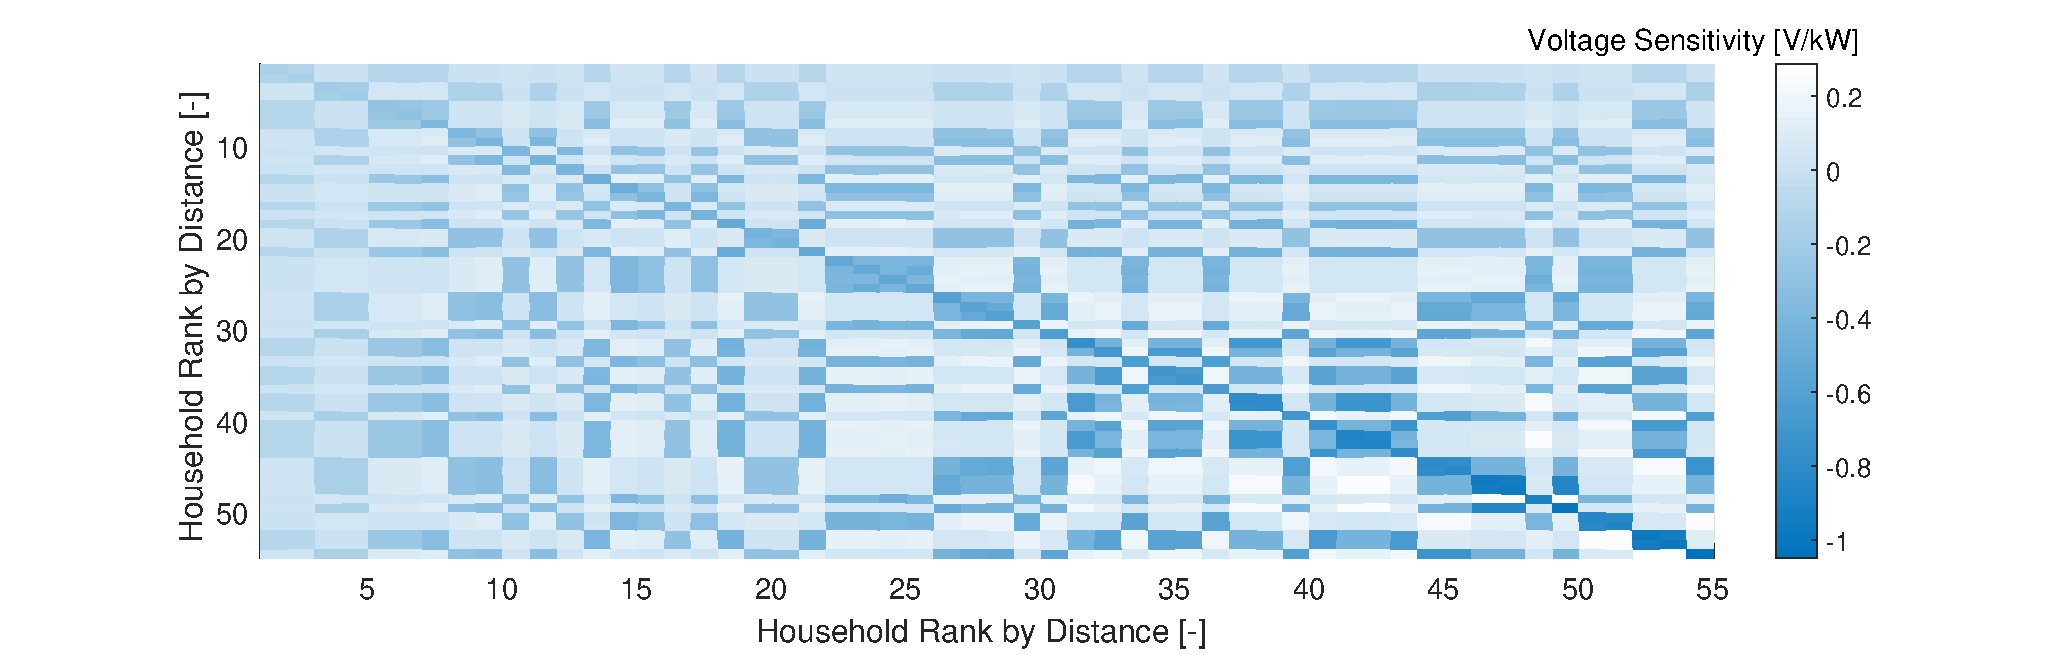
\includegraphics[width=\textwidth,trim={2cm 0cm 2cm 0cm}, clip]{figures/linear/v_sensitivity.eps}
		\label{fig:v_sensitivity}
	}
	\hfill
	\subfloat[Sensitivities of main feeder loading]{
		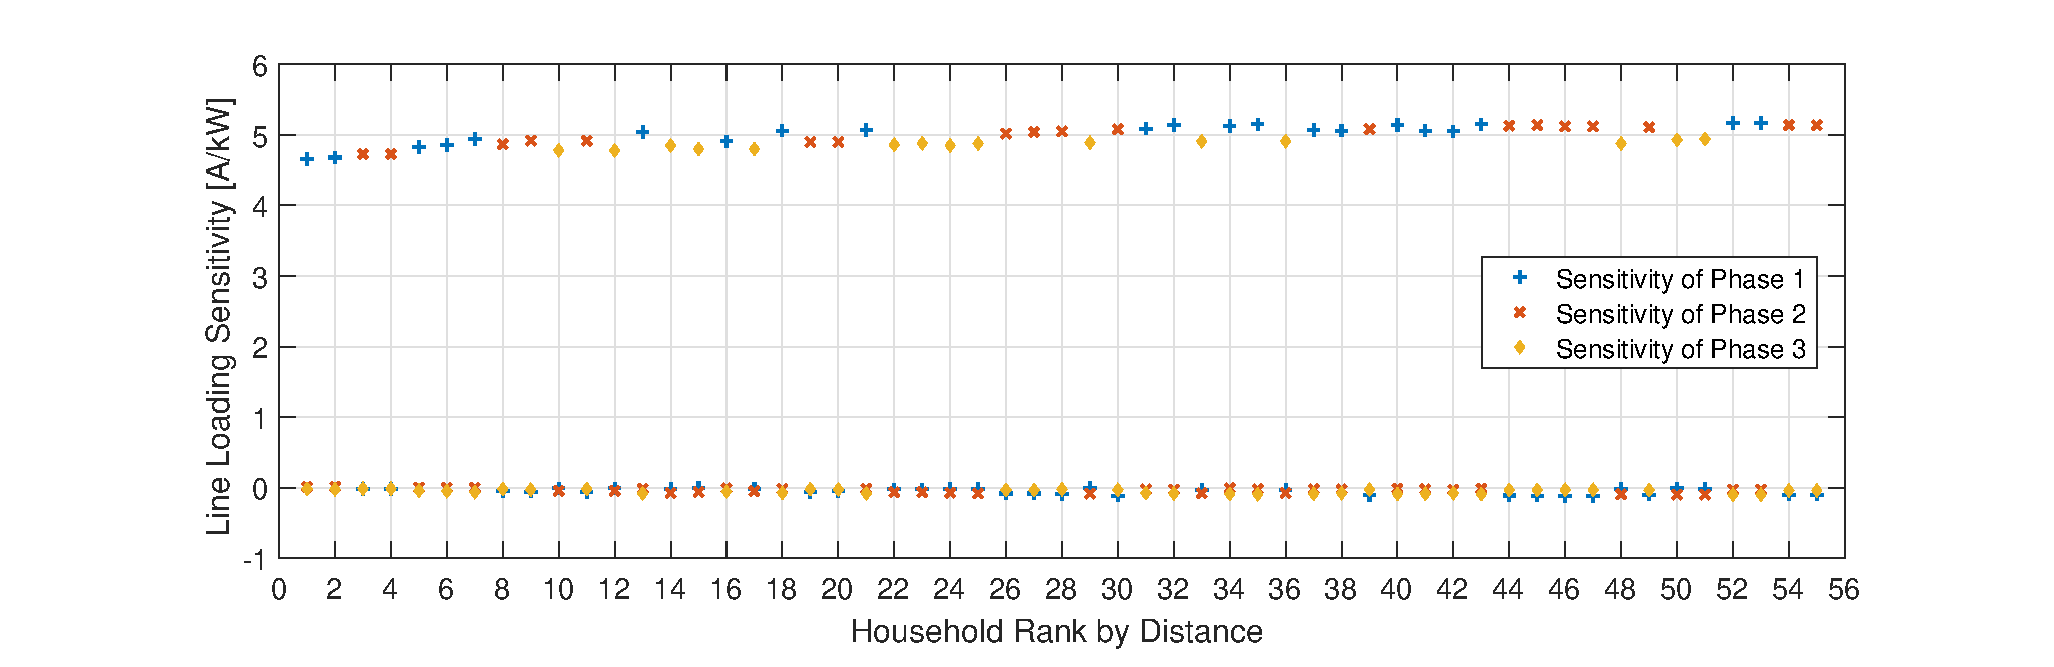
\includegraphics[width=\textwidth,trim={2cm 0cm 2cm 0cm}, clip]{figures/linear/s_sensitivity.eps}
		\label{fig:s_sensitivity}
	}
	\caption{Network sensitivities}
	\label{fig:sensitivities}
\end{figure}

% Describe sensitivity matrices
The sensitivity matrices obtained from this approach are portrayed in \Autoref{fig:sensitivities}. From \Autoref{fig:v_sensitivity} it becomes apparent that voltage drops intensify with increasing distance from the substation and focus on connections close to the location where the load is altered. The magnitude of voltage deviations ranges from -1 V/kW to 0.2 V/kW and protrude when the particular household is connected to the same phase as the point of load variation. The observed increase in phase voltages due to additional load in another phase is not uncommon in unbalanced distribution networks \cite{Richardson2012}. Similarly, the sensitivity of the primary feeder loading portrayed in \Autoref{fig:s_sensitivity} is limited to the phase at which the load is varied. Due to losses and voltage drops along the feeder a slight increase in current sensitivities can be noted with increasing distance from the substation. 

\newpage
% Describe how constraints are reformulated.
Using the voltage sensitivity matrix $\bm{\mu}$, the voltage constraint equations transform to

\begin{equation}
V_{min} \leq V^{bus}_{k,t,init}\left(\hat{D}_{k,t}\right) \;+\; \sum_{j=1}^{K} \bm{\mu}_{j,k} \cdot \pevi \leq V_{max}
\end{equation}

where $V^{bus}_{k,t,init}\left(\hat{D}_{k,t}\right)$ is the voltage resulting at the respective household and time slot due to the predicted residential demand $\hat{D}_{k,t}$ without the presence of EV loads. As this value is not altered by the decision variables, it is pre-determined as a parameter by running OpenDSS nonlinear power flow before the optimisation cycle.

Likewise, the line loading constraints are reformulated applying the line loading sensitivity matrix $\bm{\lambda}$ to each phase $r\in \{1,2,3\}$:

\begin{equation}
I_{\ell,r,t,init}^{line}\left(\hat{D}_{k,t}\right)  \;+\; \sum_{j=1}^{K} \bm{\lambda}_{j,r,\ell} \cdot \pevi \leq I_{\ell}^{max}
\end{equation}

where again $I_{\ell,r,t,init}^{line}\left(\hat{D}_{k,t}\right)$ is the current of the respective line, phase and time slot due to the predicted residential demand $\hat{D}_{k,t}$ without the presence of EV loads. Like the initial household voltages, the line loadings are calculated beforehand as parameters through OpenDSS nonlinear power flow.

% Show validity of approximation

The validity assessment of the approximation is presented in \Autoref{fig:validation_linearPF}. The data is obtained from a simulation of uncontrolled charging (cf.\ \Autoref{sec:dumbcharging}), where vehicles simply start charging upon arrival until their battery is full. The disaggregate voltage errors displayed in \Autoref{fig:voltageerrors} reveals a maximum error of only 0.3\%, prevalent underestimation of actual voltages, and naturally no errors in the absence of EV charging demand.

Additionally, analyses of the average voltage errors per time slot unveil a moderate correlation between the mean error of approximated voltages and the aggregated charging rate (\Autoref{fig:corr_schederror}). Furthermore, they show a divisive correlation between the cumulative voltage error of a household and its electrical distance from the substation (\Autoref{fig:voltageerror_hd}), reiterating the nonlinearity of power flow.

\begin{figure}[]
	\centering
	\subfloat[Disaggregate voltage error matrix]{
		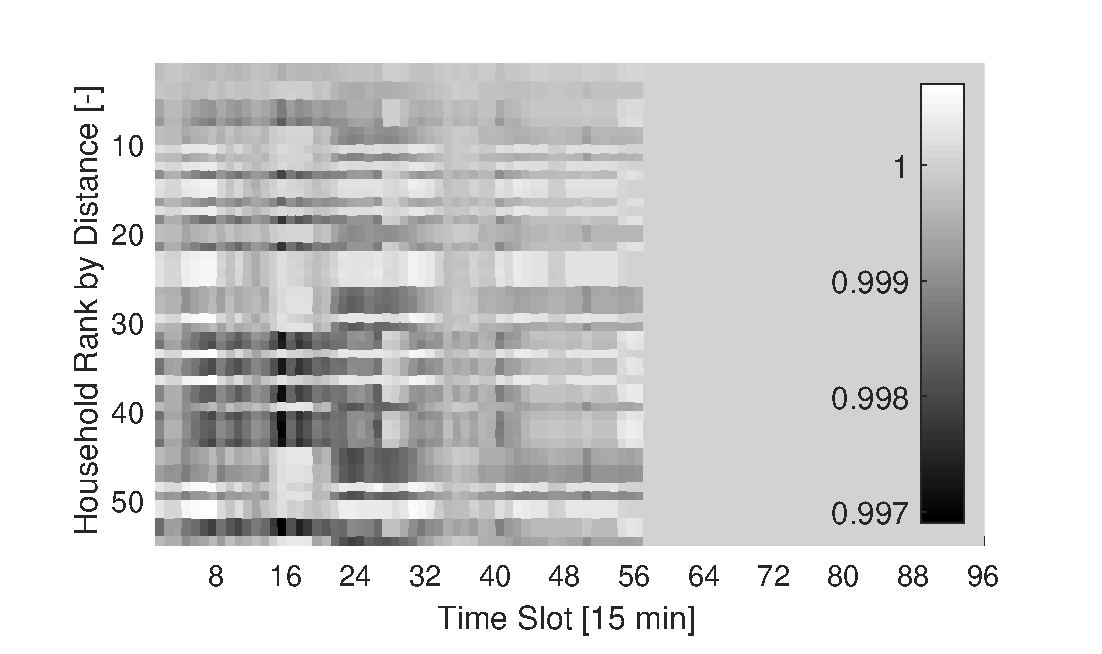
\includegraphics[width=0.48\textwidth,trim={.5cm 0cm .5cm 0cm}, clip]{figures/linear/voltageerrors.eps}
		\label{fig:voltageerrors}
	}
	\subfloat[Line loadings and errors]{
		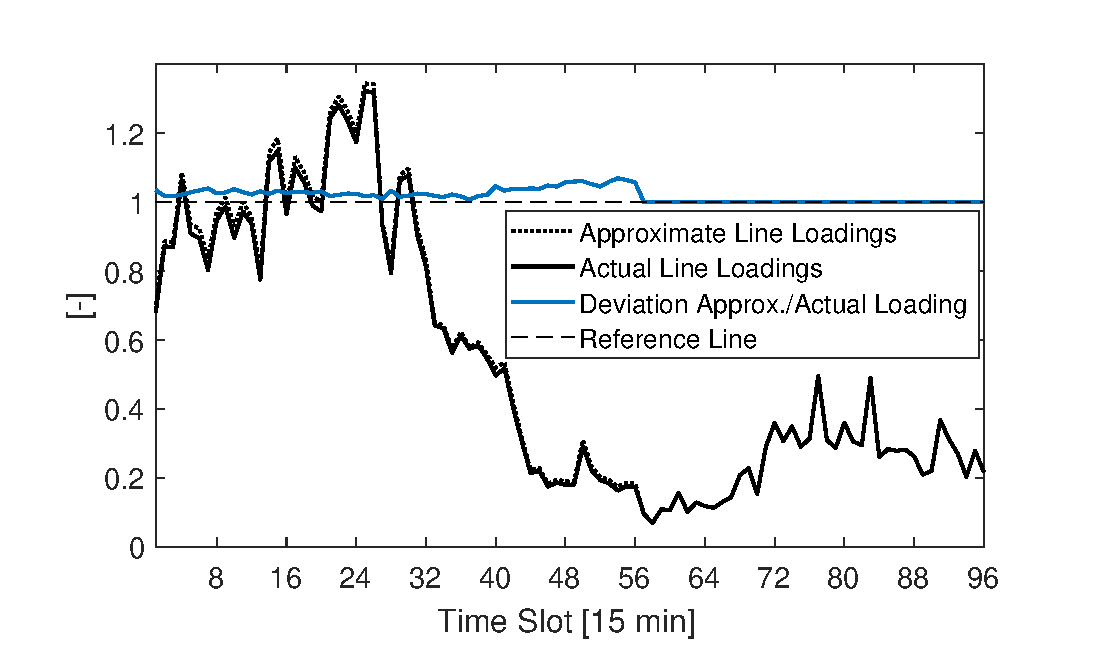
\includegraphics[width=0.48\textwidth,trim={.5cm 0cm .5cm 0cm}, clip]{figures/linear/line_error.eps}
		\label{fig:line_error}
	}
	\hfill
	\subfloat[Correlation between schedule and voltage errors]{
		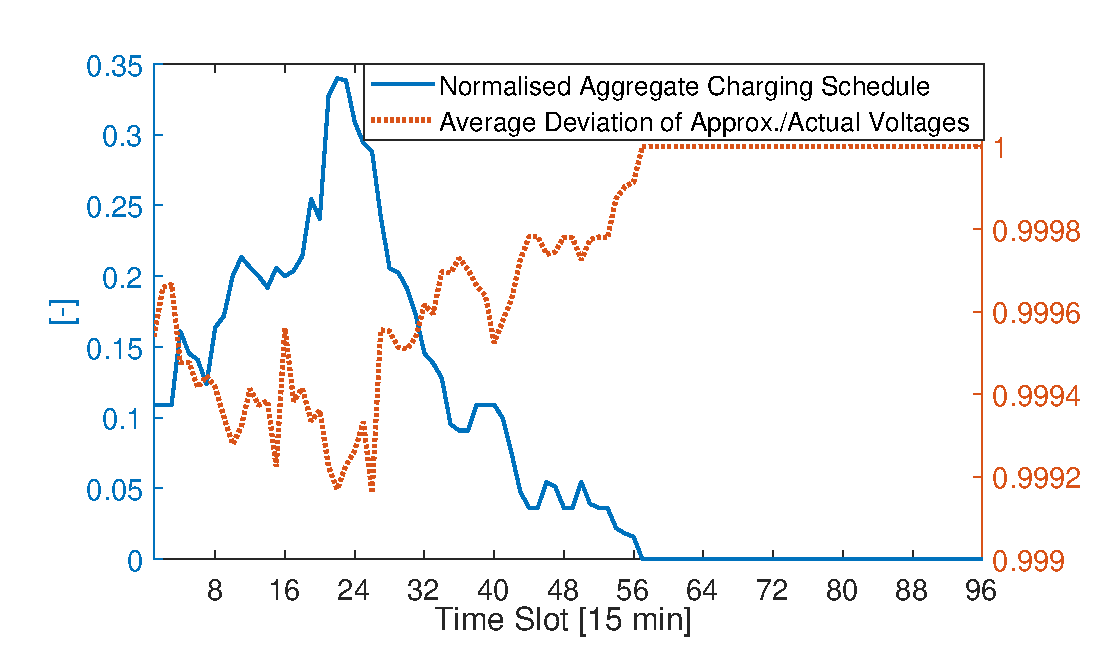
\includegraphics[width=0.48\textwidth,trim={.5cm 0cm .5cm 0cm}, clip]{figures/linear/corr_schederror.eps}
		\label{fig:corr_schederror}
	}
	\subfloat[Cumulative voltage error over time]{
		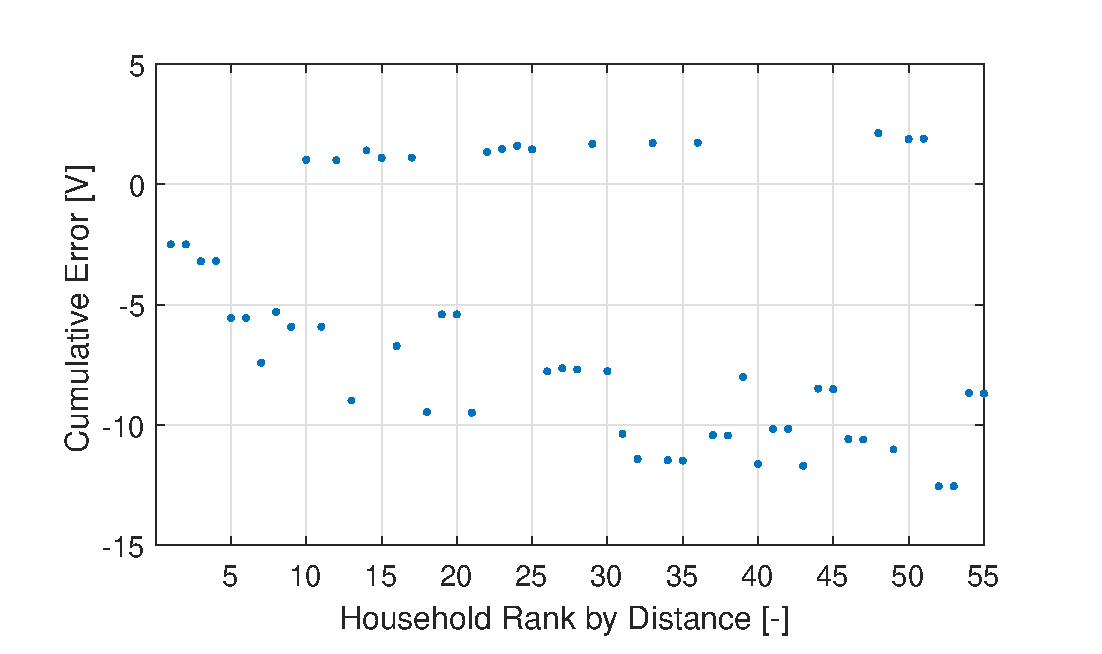
\includegraphics[width=0.48\textwidth,trim={.5cm 0cm .5cm 0cm}, clip]{figures/linear/voltageerror_hd.eps}
		\label{fig:voltageerror_hd}
	}
	\hfill
	\caption{Validation of linear power flow approximation}
	\label{fig:validation_linearPF}
\end{figure}

In line with the voltage approximations, line loadings depicted in \Autoref{fig:line_error} are slightly overestimated throughout the simulation horizon peaking at 6.8\% deviation. Overall, despite small inaccuracies the sensitivity matrices meet the requirements of a conservative approximation and are consistent with expectations, justifying their application. 

\begin{figure}[]
	\includegraphics[width=\textwidth,trim={1.5cm 0cm 2cm 0.2cm},clip]{figures/reference/dumb_ex.eps}
	\caption{Comparison of reference cases: uncontrolled charging and price-based optimisation}
	\label{fig:dumbprice}
\end{figure}

\begin{figure}[]
	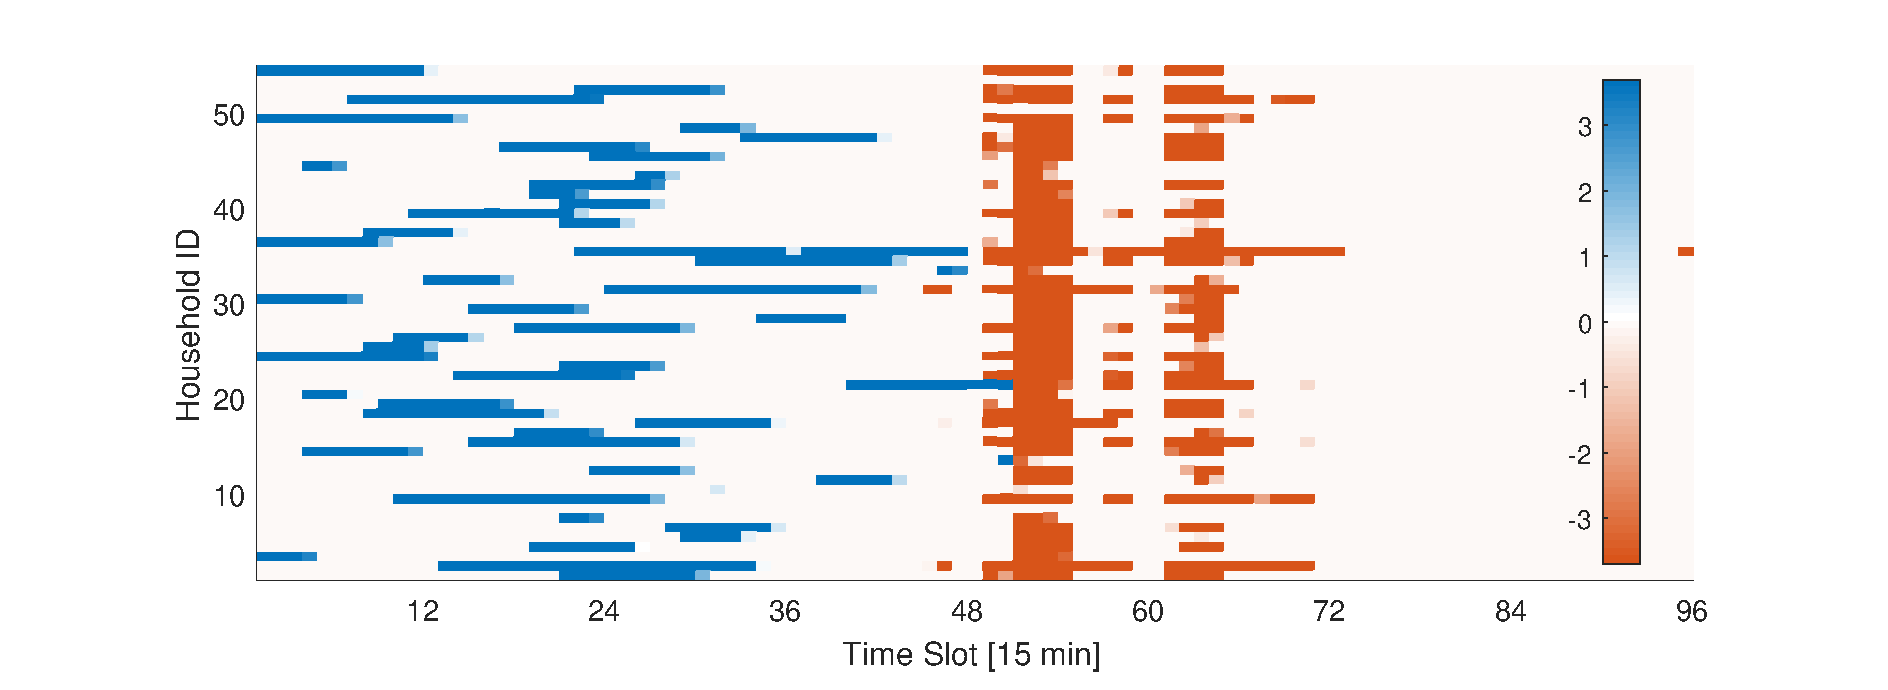
\includegraphics[width=\textwidth,trim={1.5cm 0cm 2cm 0.2cm},clip]{figures/reference/ref_scheds.eps}
	\caption{Comparison of reference cases: schedules (kW/-kW)}
	\label{fig:ref_scheds}
\end{figure}

\section{Reference Charging Approaches}
\label{sec:rc}

Two central reference charging approaches are implemented to assess the performance of the EV scheduling strategies presented in \Autoref{sec:chargecoordination}. The simulation of uncontrolled charging, commonly dubbed `dumb charging', provides a reference case for investigating the economic and technical benefits of charging coordination. Purely price-based optimisation serves as a benchmark for the costs of introducing technical network constraints.

\subsection{Uncoordinated Charging}
\label{sec:dumbcharging}

Uncoordinated charging refers to the situation where no form of control is applied, and EV loads behave as passive loads. It seeks to minimise the time to recharge the battery completely and thereby maximise the driving range available at each time slot. It is a benchmark that commonly complements the evaluation of EV scheduling approaches \cite{GonzalezVaya2015a, Galus2011, Papadopoulos2012, Wu2013, Schuller2013}.

Charging starts directly after grid connection after the last trip of the day and continues at the maximum charging rate until the battery is fully charged unless the vehicle is disconnected prematurely by the user. This `plug and charge' strategy disregards economic incentives to defer EV loads and the network state for its charging decisions.

Charging costs are evaluated based on two scenarios. First, the aggregator is obliged to purchase the inflexible aggregate demand in the market and passes the cost determined by the price time series $\pi$ on to the customers \cite{GonzalezVaya2015a}. Second, the average price $\bar{\pi}$ emulates a single-rate tariff offered by the energy utility for static loads. The latter case mirrors best the benefit an EV user would have from switching from a conventional single-rate electricity tariff to a contract with a coordinating aggregator with access to the wholesale market.

The general impact of uncontrolled EV loads has been investigated in multiple studies as summarised in  \Autoref{sec:impact}. A run of uncontrolled charging in the built model matches the analyses of previous work: \Autoref{fig:dumbprice} exposes that EV charging is centred upon periods of high residential demand, thereby causing occasional overloads and voltage violations when the aggregate of residential and EV load peaks. The coincidence of EV loads with high spot prices makes uncontrolled charging a liability for the grid integration of renewable energy sources.

\subsection{Price-Based Optimisation}
\label{sec:pbh}

A purely price-based heuristic scheduling approach serves as a reference optimisation, first, to illustrate the need for coordination of EV charging processes when access to the wholesale market is granted and, second, to quantify the cost of applying network constraints.

The scheme the heuristic follows is outlined in Algorithm \ref{alg:price}. Electricity prices are initially sorted in ascending order from lowest to highest values, and a charging schedule is determined independently for each electric vehicle. No coordination between EVs takes place, and schedules can be achieved without information exchange to a third-party agent. Among the slots in which a particular vehicle is plugged in, starting with the cheapest slot charging rates are set to their maximum in the next cheapest slot until the battery is completely charged.

\begin{algorithm} 
	\caption{Price-based Heuristic Scheduling}
	\begin{spacing}{1.2}
		\begin{algorithmic}[1]
			%\Require $\pi\in\mathbb{R}^T$, the simulated price time series
			\State Sort prices $\pi\in\mathbb{R}^T$ in ascending order $\sigma \in \mathbb{N}^T$
			\State Initialise empty vehicle charge schedules: $P^{EV} = \bm{0}_{K,T}$
			\ForEach {household $k \in K $}
			\State {Determine vehicle energy demand: $D^{EV}_k \gets B_{max} - B^{arr}_k$}
			\ForEach {time slot $t \in T $}
			\While {$D^{EV}_k > 0$}
			\If{$\alpha^{EV}_{k,\sigma(t)} = 1$}
			\State {$P^{EV}_{k,\sigma(t)} \gets \min\left\{P_{max}, \frac{D^{EV}_k}{\eta \cdot \Delta t}\right\}$}
			\State {$D^{EV}_k \gets D^{EV}_k - P^{EV}_{k,\sigma(t)} \cdot \eta \cdot \Delta t$}
			\EndIf
			\EndWhile
			\EndFor
			\EndFor
			\State \Return {complete vehicle charge schedules: $P^{EV}\in \mathbb{R}^{K\times T}$}
		\end{algorithmic}
	\end{spacing}
	
	\label{alg:price}
\end{algorithm}

This greedy heuristic, when applied with perfect forecasts, produces a schedule causing the least charging costs possible to satisfy user demands given the EV availability periods. Because prices may be the same in multiple time slots, different optimal schedules are conceivable but would ultimately result in the same minimal charging costs for the given model. These costs are a lower bound against which any charging costs obtained by algorithms considering additional constraints (e.g.\ concerning network state or conservation of EV batteries) can be assessed.

The comparison with the uncontrolled charging approach in \Autoref{fig:dumbprice} reveals a tendency for high concentration of loads in cheap time slots. This is because every EV agent is assumed to act rationally towards her maximum economic benefit and low prices happen to intersect with the availability periods of EVs. In comparison to uncontrolled charging, this may lead to even more severe voltage violations and mains cable overloading. Consequently, without local adaptation of electricity prices to reflect the state of the low-voltage distribution network by means such as locational marginal pricing (LMP), purely price-based charging might balance the volatility of renewable generation and electricity demand but not foster high capacity exploitation and load accommodation in distribution networks. New load peaks due to low price signals in distributed optimisation may be alleviated by applying physical constraints.

\section{Charge Rate Coordinating Scheduling Methods}
\label{sec:chargecoordination}

%Explain need for coordination

Evidently, both uncontrolled EV charging and price-based heuristic scheduling fail to observe statutory voltage limits and thermal line ratings at all times and are inept to guarantee a safe network operation. However, the dual role of the aggregator not only entails a commitment to the economic benefit and demand satisfaction of individual consumers but also the technical requirements of the distribution network operator. While the two reference cases excel at reliably re-charging batteries, by violating network constraints the aggregator puts its obligation to the distribution system operator in second place. Thus, two methods incorporating system constraints were developed: a linear program and a heuristic optimisation extending upon the price-based reference methods. 

\subsection{Linear Programming}

Thanks to the linear power flow approximation through network sensitivities introduced in \Autoref{sec:lpf} the EV scheduling problem can be easily and quickly solved by a linear program. In this work, Gurobi is used as a solver and embedded in the simulation framework. Except for the limitations induced by possible prediction errors and the linear power flow approximation, the solver will produce the best coordination of EV charging processes regarding both \textit{when} and \textit{which} EVs should charge. Due to the centralised approach to scheduling, it requires significant information exchange of input parameters between customer and aggregator and likely entails poor scalability.

\subsection{Network-Constrained Price-Based Heuristic Optimisation}

Other than the centrally organised linear program, in the extended price-based heuristic (\Autoref{sec:pbh}) cost-minimising schedules are determined locally without prior knowledge of the network conditions and submitted to the aggregator. Subsequently, the aggregator checks whether the new schedule in addition to previously committed schedules and demand forecasts causes any voltage issues or exceeds network capacities. If violations occur, the aggregator rejects the schedule and imposes a suitable load limitation signal according to which the vehicle is rescheduled locally. Otherwise, the schedule is adopted, and the aggregator awaits the schedule proposal of the next electric vehicle. This process is repeated iteratively until all electric vehicles are scheduled. Full insight into the functioning principle of the heuristic is provided in Algorithm \ref{alg:ncpbh}.

Because the order by which EV schedules are taken influences the performance of the heuristic, several cases are examined where the priority list $\theta \in \mathbb{N}^K$ is determined

\begin{itemize}
	\item by EV arrival time in ascending order,
	\item by EV availability period in ascending order,
	\item by EV battery state of charge upon arrival in ascending order,
	\item by electrical distance of household from substation in ascending order, or
	\item by electrical distance of household from substation in descending order.
\end{itemize}

Prioritising by \textit{arrival time} constitutes an easy escape from arrival and battery state of charge uncertainty if power can be traded on an intraday market and schedules are proposed and checked by the aggregator upon arrival in real time.

Sorting by the expected \textit{availability period} or the \textit{initial battery state of charge} of an electric vehicle ranks the vehicles by their degree of load flexibility. It avoids that an inflexible electric vehicle cannot be fully loaded because all its charging options are exhausted as limits in the network are reached. The primary motive is to achieve a high demand satisfaction rate.

Sorting by \textit{ascending electrical distance} aims at accommodating the maximum amount of EVs in inexpensive time slots. This makes use of the observation that due to the radial layout of the distribution network voltage levels are less sensitive to the addition of loads near the substation \cite{Richardson2012}. Conversely, A priority list based on \textit{descending electrical distance} should expose significantly lower energy delivery in the cheapest slots. This approach makes price reduction a priority and might result in electric vehicles at the end of the feeder paying higher rates for charging due to load limitation signals in already fully exploited inexpensive slots. This inequality would require a fair cost redistribution through the aggregator.
 
\begin{algorithm}[h]
	\caption{Network- and Price-Based Heuristic Scheduling}
	\label{alg:ncpbh}
	\begin{spacing}{1.2}
	\begin{algorithmic}[1]
		%\Require $\pi\in\mathbb{R}^T$, the simulated price time series
		\State Sort prices $\hat{\pi}\in\mathbb{R}^T$ in ascending order $\sigma \in \mathbb{N}^T$
		\State Determine order $\theta\in  \mathbb{N}^K$ by which vehicles are scheduled
		\State Initialise empty vehicle charge schedules: $P^{EV} = \bm{0}_{K,T}$
		\ForEach {household $k \in K$}
		\State {Determine vehicle energy demand: $D^{EV}_{\theta(k)} \gets B_{max} - B^{arr}_{\theta(k)}$}
		\State {Initialise set of charging rate limits induced by network state: $P_{max}'= (P_{max})_{K,T}$}

		
		\While {$\neg\forall \ell\in L, t\in T, k\in K\; V_{min} \leq V_{k,t}^{bus} \leq V_{max} \text{ and } I_{\ell,p,t}^{line} \leq I_{\ell}^{max}$}
		\ForEach {time slot $t \in T $} %\Comment{Calculate greedy schedule proposal}
		\While {$D^{EV}_{\theta(k)} > 0$}
		\If{$\alpha^{EV}_{{\theta(k)},\sigma(t)} = 1$}
		\State {$P^{EV}_{{\theta(k)},\sigma(t)} \gets \min\left\{P_{max}, \frac{D^{EV}_{\theta(k)}}{\eta \cdot \Delta t}\right\}$}
		\State {$D^{EV}_{\theta(k)} \gets D^{EV}_{\theta(k)} - P^{EV}_{{\theta(k)},\sigma(t)} \cdot \eta \cdot \Delta t$}
		\EndIf
		\EndWhile
		\EndFor
		
		%\Comment{Check proposed schedule for infeasibilities and mitigate}
				
		\If {$\neg\forall \ell\in L, t\in T, k\in K:\; V_{min} \leq V_{k,t}^{bus} \leq V_{max} \text{ and } I_{\ell,p,t}^{line} \leq I_{\ell}^{max}$}
		\State Find set of slots $T_{viol}\subset T$ with technical violations
		\ForEach {$\tau \in T_{viol}$}
		\State {$P_{max,\theta(k),\tau}' \gets P^{EV}_{\theta(k),\tau}-\Delta P$} \Comment {$\Delta P$ denotes step size of load limitation}
		\If {$P_{max,\theta(k),\tau}' \leq 0$}
		\State {$\hat{\pi}_\tau \gets \infty$}
		\EndIf
		\EndFor
		\State Re-sort prices $\hat{\pi}\in\mathbb{R}^T$ in ascending order $\sigma \in \mathbb{N}^T$
		\State Reset schedule: $P^{EV}_{{\theta(k)},\sigma(t)} \gets 0$ for all $t \in T$
		\EndIf
		
		\EndWhile
		

		\EndFor
		\State \Return {complete vehicle charge schedules: $P^{EV}\in \mathbb{R}^{K\times T}$}
	\end{algorithmic}
	\end{spacing}
	\label{alg:network}
\end{algorithm}

Other than the linear program, the network-constrained heuristic does not require a linear power flow approximation but can retrieve accurate voltage and line loading measurements directly from the OpenDSS simulation. Moreover, it constitutes a slightly more decentralised approach involving less information exchange improving privacy preservation and scaling-induced complexity because schedule proposals are now determined locally, and the aggregator only monitors the status of the distribution network. Due to the lack of formality in heuristic optimisation, there is no guarantee for an optimal solution. Nevertheless, the evaluation of priority lists will support the understanding of the primary determinants affecting the optimal charging coordination of electric vehicles, which the linear program lacks to illustrate.

\section{Approaches to Uncertainty Mitigation}
\label{sec:uncmitigation}

% uncertainties involved and assumptions

Because EV charging coordination is embedded in a highly stochastic environment but most decisions may have to be taken before observing realisations of uncertain parameters, optimisation based solely on expectation values is not robust and offers potential to extenuate sensitivities towards forecast deviations. Consequently, this section introduces uncertainty mitigation options which are subsequently evaluated in \Autoref{sec:saunc}. Note that the presented concepts rely on the assumption that based on the empirical data of a user, probabilities for input parameters can be defined similarly to the modelled distribution functions, conscious that this was yet another modelling approximation. 

Classical \textit{robust optimisation} is a method for risk-averse decision making yielding the least worse outcome. It is commonly applied when parameters are known only within certain bounds, and uncertainty preponderates in constraints. Its primary goal is to find undoubtedly feasible solutions, whereas optimisation is just the secondary objective. The high level of conservatism involved may incur substantial cost increases \cite{Bertsimas2004}. 

Quantifying the uncertainty in the true value of a parameter by empirical or idealised probability distributions allows \textit{stochastic programming}. This method requires much more insight into historical consumption patterns and extends robust optimisation \cite{Sim2017}. Other than robust optimisation, however, its goal is to find an optimal solution that is feasible for almost all possible parameter sets, relaxing the usually expensive worst case consideration. For heavily interwoven uncertainties, where the interlink between parameters is unknown, it is common to reduce complexity via a scenario tree by extracting at random some instances of the uncertain parameters and find a feasible solution for these samples. For the scheduling of electric vehicles, the adversity of parameter uncertainties can largely be quantified and identified separately, so that individual security margins for unfavourable cases of a particular parameter can be defined. Although no financial weighting between constraint satisfaction and cost minimisation is assumed, applied security margins provide the ability to mimic appropriate weightings. Further, it should be noted despite attempting to mitigate uncertainty, the optimisation routine is deterministic and recognises the stochasticity of the problem by adapting its input parameters only according to the pre-calculated probability distributions.

% TODO check and cite some things

\subsection{Availability Uncertainty}
\label{sec:av_unc}

Uncertainty about the arrival and departure times of electric vehicles can be defused using the historical mobility profile of an EV owner. Instead of using the expectation values as forecasts, $\hat{\alpha}^{EV}_{t}$ may indicate time slots in which the availability probability $\mathbb{P}\left(\alpha_t^{EV}=1\right)$ is larger than a given threshold. As outlined in \Autoref{sec:mub}, the availability probability is calculated from the CDFs of the arrival and departure time distributions and is illustrated in \Autoref{fig:av_mit}. While choosing a high threshold demanding a degree of certainty of $\nu_{\alpha}$ reduces charging flexibility by narrowing the predicted availability period, it also reduces the chances of an electric vehicle scheduled to charge in times where it is not available. At the cost of missing cheap slots where the car actually turns out to arrive earlier or depart later than predicted, the robustness to forecast deviations is increased in terms of fulfilling customer demand for a full battery. Thus,

\begin{equation}
\hat{\alpha}'^{EV}_{t} = \begin{cases}
1 & \text{if  }\mathbb{P}\left(\alpha^{EV}_{t}=1\right) \geq \nu_{\alpha} \\
0 & \text{else}
\end{cases}
\end{equation}

% An alternative to (penalty) defines the cost of 

\begin{figure}[]
	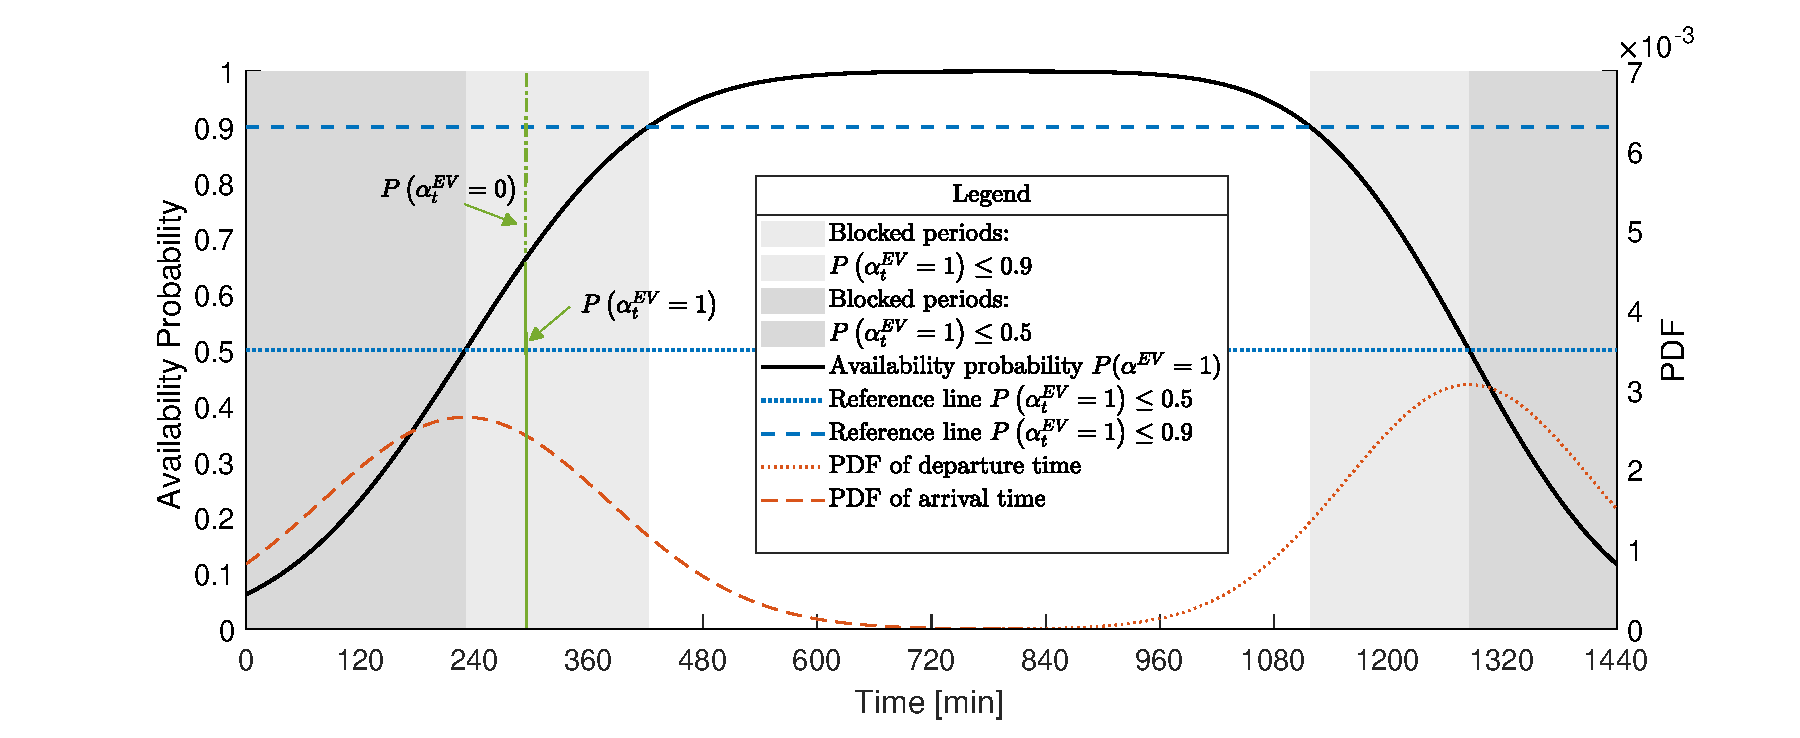
\includegraphics[width=\textwidth,trim={1.5cm 0cm 1.5cm 0.2cm},clip]{figures/mitigation/av_mit.eps}
	\caption{Approaches for the mitigation of availability uncertainty}
	\label{fig:av_mit}
\end{figure}

\subsection{Battery Charge Level Uncertainty}

Uncertainty mitigation concerning the battery state of charge upon arrival in day-ahead scheduling is likewise rested on historical mobility profiles of individual EV users. Deviation from the maximum likelihood estimator as a forecast value $\hat{B}^{arr}$ involves a trade-off between the risk of not fully charging a battery if the SOC is less than predicted and excessive scheduling if the SOC is higher than expected for robustness, thereby blocking eventually fallow network capacity. The issue is depicted in \Autoref{fig:soc_mit}. Assuming a state of charge exceeded in a ratio of $\nu_{B}=0.7$ of all cases instead of its actual expectation value will increase the likelihood of curtailment due to a full battery achieved prematurely. Prioritising customer satisfaction over reduced capacity and price exploitation, sensitivity analysis in \Autoref{sec:saunc} focusses on the cost of excessive scheduling.

\begin{figure}[]
	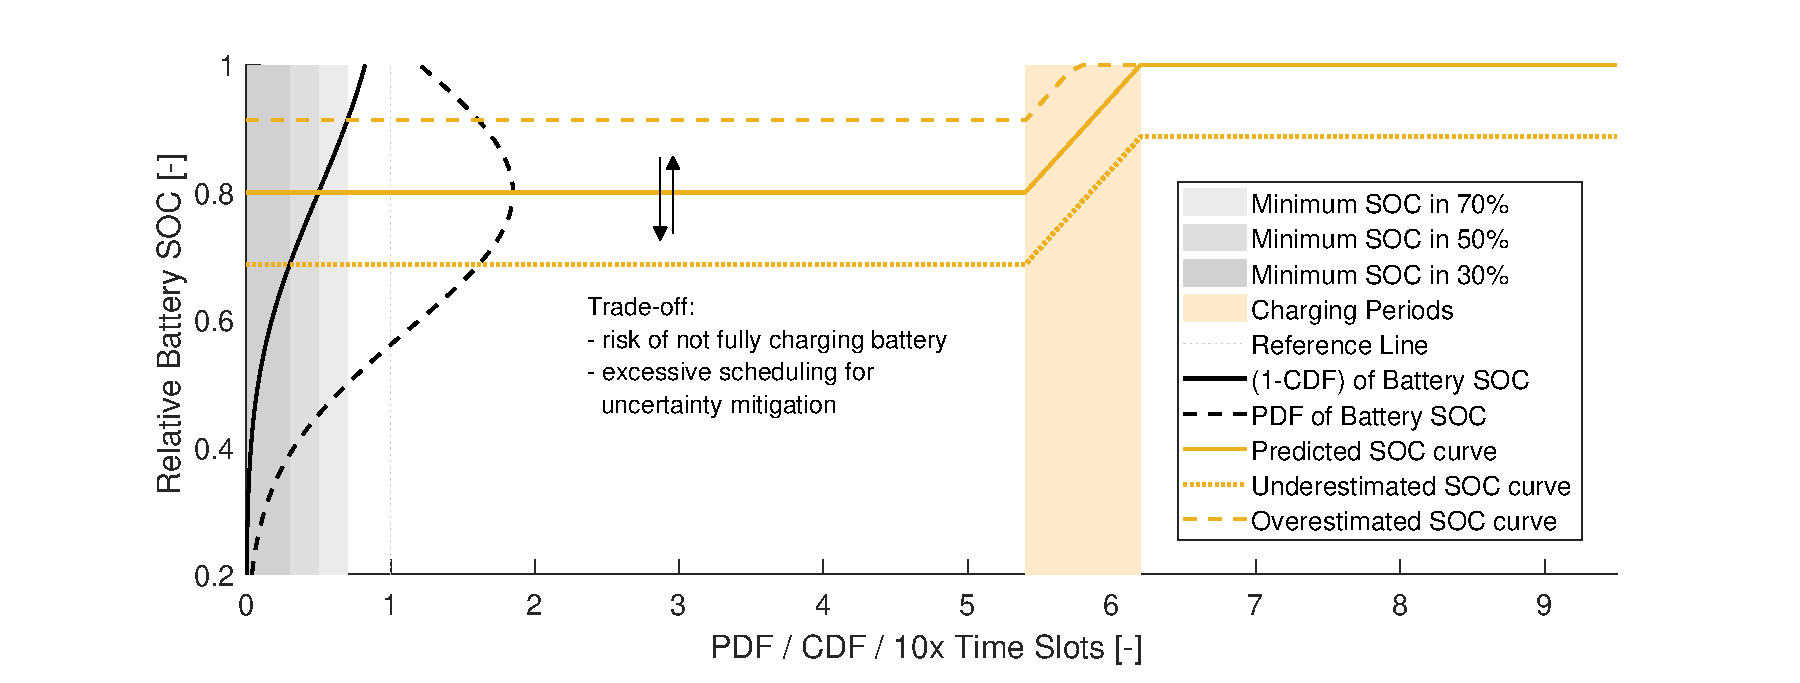
\includegraphics[width=\textwidth,trim={2.1cm 0cm 2.1cm 0.2cm},clip]{figures/mitigation/soc_mit.eps}
	\caption{Mitigation of battery state of charge uncertainty}
	\label{fig:soc_mit}
\end{figure}

\subsection{Spot Price Uncertainty}

Mitigation of price uncertainties relies on the assumption that forecasts can be given with certain error margins and distributions. Furthermore, it is clear that uncertainty of price time series is only relevant if the ranking is distorted significantly and hedging against severe underestimation of prices is a priority for risk-averse aggregators. Instead, expectation values could be replaced by their $\nu_{\pi}$-quantiles as the price input for each time slot. This quantile refers to the rate which is not exceeded in $100\cdot\nu_{\pi}$ \% of cases. Although this input deviates from the best estimator for electricity prices, it reflects the extent of involved uncertainties by deferring highly uncertain time slots to rearward positions in the price ranking. Thereby, it disincentivises a scheduling algorithm to charge in cheap but uncertain slots and increases the robustness of the schedules against adverse realisations of electricity prices. 

For the exemplary price profile of \Autoref{sec:pr_unc}, \Autoref{fig:pr_mit} visualises the quantiles and ranking distortion compared to the 0.5-quantile. Approximating the worst-case scenario, the ranking distortion measured by the Spearman's rank correlation coefficient intensifies. Nonetheless, the correlation coefficients also expose very limited variation in the ranking. Per design, the cost of mitigation arises from the diminished opportunity to exploit low prices in uncertain time slots.

\begin{figure}[]
	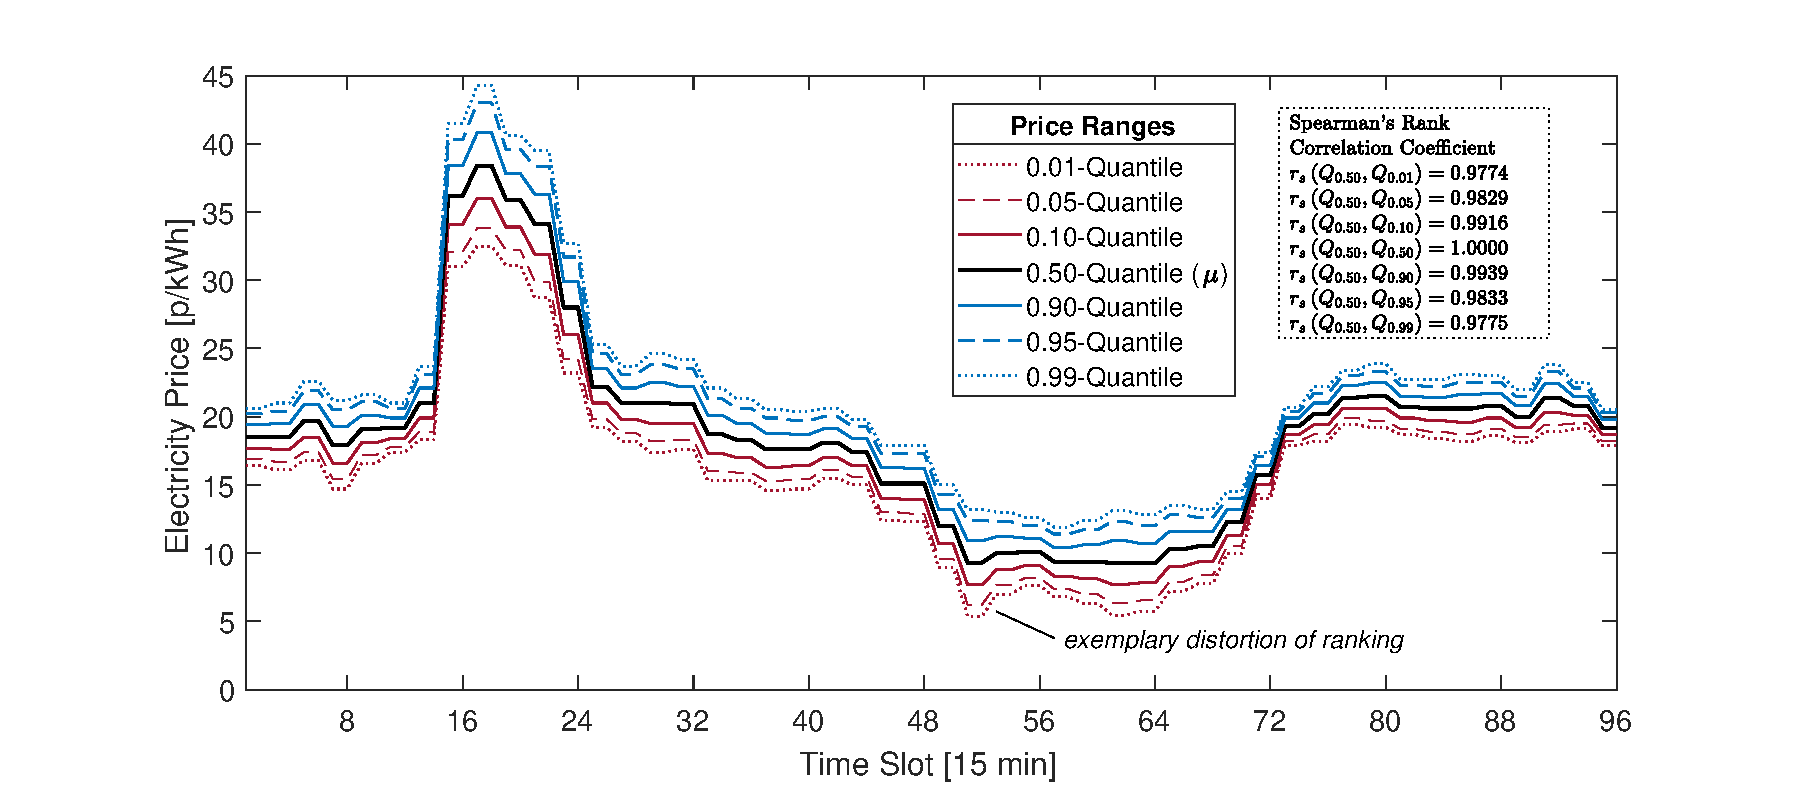
\includegraphics[width=\textwidth,trim={2.1cm 0cm 2.1cm 0.2cm},clip]{figures/mitigation/pr_mit.eps}
	\caption{Approaches to mitigation of price uncertainties}
	\label{fig:pr_mit}
\end{figure}

\subsection{Residential Demand Uncertainty}

In \Autoref{sec:rd_unc} it has been discussed that uncertainty \textit{when} dominates uncertainty about \textit{what} residential demand peaks occur and demand profiles may randomly shift within a certain time frame. Robustness against demand uncertainty is achieved by building a rolling maximum from expected residential loads to form the new demand forecast

\begin{equation}
\hat{D}_t' = \max \left\{\hat{D}_i \;|\; i \in \{t-w_{max},\dots,t,\dots,t+w_{max}\}\right\},
\end{equation}

where $w_{max}$ is the presumed maximum deviation between predicted and simulated demand. Set to 30 minutes in either direction, the adapted residential demand output compares to the prediction as shown in in \Autoref{fig:dem_mit}. This protects the schedule from causing overloads and voltage problems due to residential loads deviating within the window size by anticipating their occurrence in any possible slot. As this approach reduces the available capacity for EV charging, cost increases are foreseen. 

\begin{figure}[]
	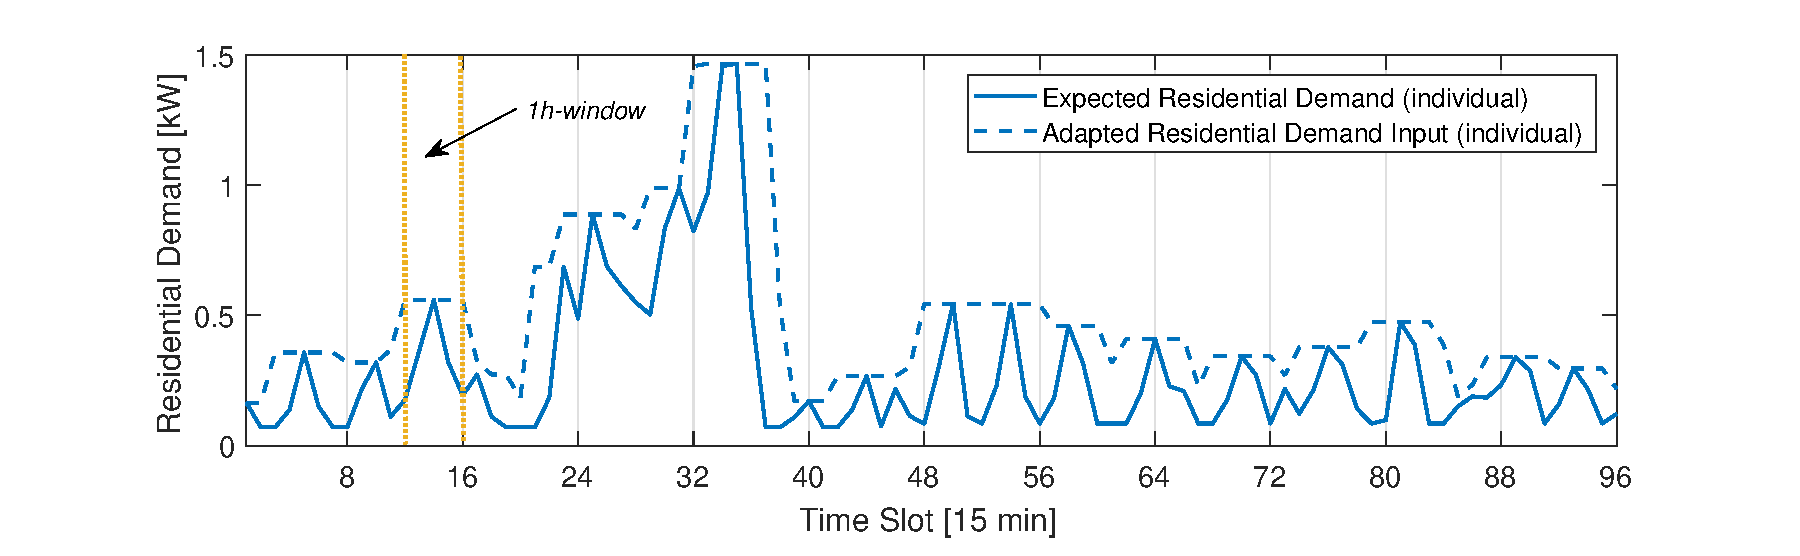
\includegraphics[width=\textwidth,trim={2.1cm 0cm 2.1cm 0.2cm},clip]{figures/mitigation/dem_mit.eps}
	\caption{Illustration of demand uncertainty mitigation}
	\label{fig:dem_mit}
\end{figure}
\addtocontents{toc}{\protect\newpage}
\chapter{Evaluation}
\label{sec:eval}

This chapter investigates the performance of presented approaches and variants to EV scheduling in relation to the pre-defined reference cases, summarised in \Autoref{tab:casestuds}. In \Autoref{sec:ec} the characteristics of the reference optimisations are reiterated, and evaluation criteria whereby effectiveness will be assessed are introduced. \Autoref{sec:hmlp} compares the performance of different configurations of network-constrained heuristics and linear programming before uncertainty mitigation options are applied in \Autoref{sec:saunc}. Parametrisation options are, first, interpreted individually and then applied conjointly in \Autoref{sec:joint}. While the preceding sections judge based on the aggregate of 20 scenarios corresponding to a four week weekday period to hedge against the variability of performances across different situations, \Autoref{sec:sceneval} picks a single scenario for an in-depth analysis. \Autoref{sec:hdeval} provides insight into peculiarities on an individual household level before results are discussed, and potential is analysed in \Autoref{sec:pseval}. This is associated with a sensitivity analysis of market price spreading factors towards cost savings.

\begin{table}[]
	\centering
	\scriptsize
	\begin{tabular}{@{}lllll@{}}
		\toprule
		\textbf{Case Studies}  & \textbf{Variants}        &                         &                       &                             \\ \midrule
		Reference Cases        & No Electric Vehicles     & Uncontrolled Charging   & Price-Based Heuristic &                             \\ \midrule
		Heuristics             & Availability             & Battery SOC             & Distance (asc.)       & Distance (desc.)            \\ \midrule
		Linear Programming     & Unconstrained Modulation & Constrainted Modulation & Combined Mitigation   &                             \\ \midrule
		Uncertainty Mitigation & \textit{Availability}    & \textit{Battery SOC}    & \textit{Market Price} & \textit{Res. Demand} \\  \cmidrule{2-5}
		& $\nu_\alpha = 0.6$       & $\nu_B = 0.6$           & $\nu_\pi = 0.90$      & $w = 0.5 $ h                 \\
		& $\nu_\alpha = 0.7$       & $\nu_B = 0.7$           & $\nu_\pi = 0.95$      &                             \\
		& $\nu_\alpha = 0.8$       & $\nu_B = 0.8$           & $\nu_\pi = 0.99$      &                             \\ \bottomrule
	\end{tabular}
	\caption{Summary of evaluated case studies}
	\label{tab:casestuds}
\end{table}

\section{Evaluation Criteria and Reference Cases}
\label{sec:ec}

To facilitate a concise comparison between the scheduling approaches, boxplots are used to indicate the distributions (illustrated by quartiles and whiskers) and averages (denoted by circles) of evaluation criteria throughout the 20 scenarios. Particularly concerning costs, the results are set in relation to the results of uncontrolled charging and the purely price-based heuristic. Recall that three major areas of concern determine the performance of a scheduling approach: cost savings from devised charging, a full battery at the end of the charging period, and the observation of network constraints. These lead to the following evaluation criteria which are inspected separately as no trade-offs are quantified.

\begin{itemize}
	\item \textbf{Relative charging costs} offer insight into the economic benefit of coordinated charging compared to uncontrolled charging as well as a proxy for the costs of introducing network constraints if compared to unconstrained price-based charging.
	\item \textbf{Demand satisfaction} is measured by both the average and minimum final battery state of charge of the controlled vehicles. The latter gives an indication of an algorithm's reliability to provide a minimum driving range to the customer.
	\item \textbf{Severity of constraint violations} is quantified by maximum line loadings and the minimum bus voltages occurring at the households throughout the optimisation horizon.
	\item \textbf{Frequency of constraint violations} is measured by relating the number of overloads or voltage violations to the total number of values measured.
\end{itemize}

\begin{figure}[]
	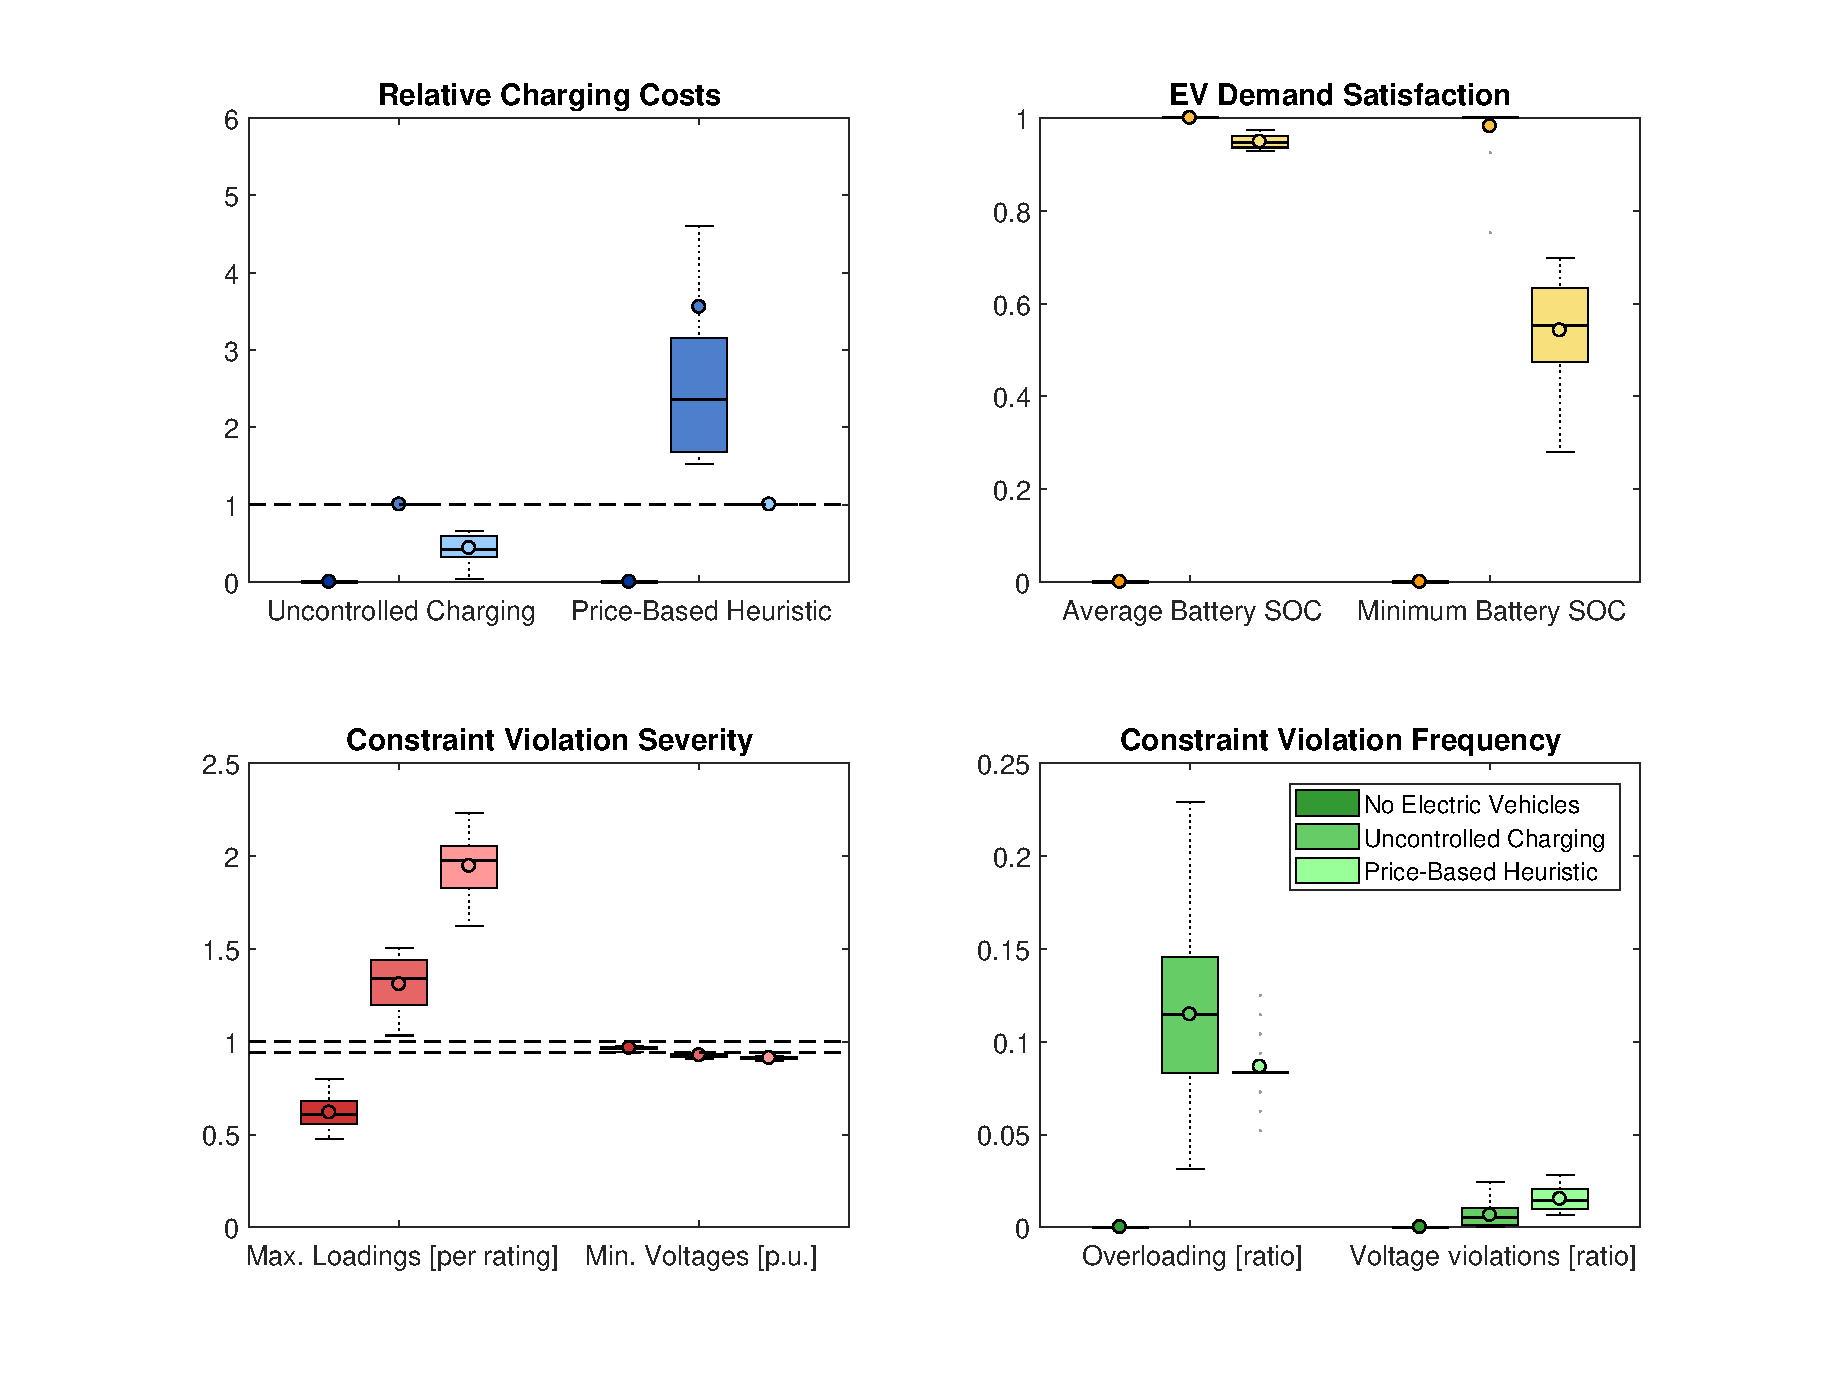
\includegraphics[width=\textwidth,trim={3cm 1.5cm 2.5cm 0cm},clip]{figures/evaluation/refcases.eps}
	\caption{Benchmark of reference cases: no EVs, uncontrolled charging, and price-based heuristic}
	\label{fig:refcases}
\end{figure}

Initially, a look at the performance of the benchmarks in \Autoref{fig:refcases} affirms their unsuitability to achieve safe, reliable, and cheap EV charging. While the price-based heuristic excels at reducing charging costs to about one half compared to uncontrolled charging, it fails to guarantee a full battery state of charge which is due to the day-ahead scheduling involving uncertain parameters. Conversely, the uncontrolled charging stands out with its advantage of operating in real-time and can almost guarantee a full battery. Still, the possibility exists that charging cannot be completed for the EV availability is too limited. Despite the shortcomings of day-ahead scheduling, an average fulfilment ratio of vehicle demand of 94.86\% is considerable and covers most daily trip lengths. However, due to reliability concerns the minimum battery SOC is the more critical performance measure influencing customer acceptance, which averages at only 54.17\%.

\newpage
A glance at the maximum line loadings and minimum voltages reveals that without electric vehicles the test network is perfectly healthy; no violations occur. Yet, the presence of uncontrolled EV charging causes voltage violations and overloads in any scenario averaging at an excess loading of 30.84\%. Due to the natural spread of arrival times, the overloads are nowhere near the overloads caused by applying the price-based heuristic averaging at a 94.63\% excess loading. Analogous findings could be made for minimum bus voltages. The fact that charging concentrates in the single cheapest slots coupled with high availability rates reiterates the need for charging coordination of electric vehicles if general price-based incentives are given.

In terms of violation frequency, the price-based heuristic also entails more voltage issues than uncontrolled charging because the high peak loads -- in addition to the increased likelihood \textit{that} a voltage violation occurs -- not only deteriorates voltages locally but will also propagate along the feeder. Because of the peakiness of the schedule overloads of the mains cable are less frequent than invoked by uncontrolled charging, again due to the natural arrival time spread. While loads still occur in periods of peak residential demand, they distributed over that period such that line limits are continuously exceeded.

\section{Performance of Heuristic Modes and Linear Programming}
\label{sec:hmlp}

Having analysed the reference cases, the different network-constrained heuristic modes were run as outlined in the introduction to this chapter, with priority lists determined by the rank of availability period, initial SOC, ascending or descending distance from the substation. \Autoref{fig:heulp} summarises the performance of applied charging schemes. Relatively similar charging costs are achieved regardless of the priority list used by which EVs are scheduled. All were able to reduce costs by approximately 54\% compared to uncontrolled charging for the given market assumptions (spreading factor $s=5$), the sensitivities to which are addressed later in \Autoref{sec:pseval}. Noteworthily, other than expected the ordering by ascending distance does not improve costs, and no financial benefit could be drawn from maximum capacity exploitation in cheap slots. Instead, prioritising by initial SOC convinces with a slight advantage of 1\% with respect to cost increase due to technical constraints. The lower deviation of the price-based heuristic costs by the network-constrained variants is obtained through favourable price forecast variations in slots where the latter charges more than the former and this would not be possible if no uncertainty were involved. While the average fulfilment ratio of EV demands remains indistinguishable at 94.80\% across different heuristic configurations, the minimum reached battery charge level of vehicles under the aggregator's control is minimally less for mode `SOC' and `descending distance'.

Concerning the technical performance of the heuristic modes, it can be noticed that the marginal economic advantage of mode `SOC' is paid with an increased risk of overloading of the mains cable and local voltage violations. Although in the vast majority of cases network constraints are observed, they are not precluded. Importantly, other than for the uncoordinated reference cases, overloads induced by the network-constrained heuristics are limited to marginal overloads of up to 2\% which are most likely due to an unfavourable shift in residential loads. The linear power flow approximation continued to yield overestimates and did not contribute to these overloads.

\begin{figure}[]
	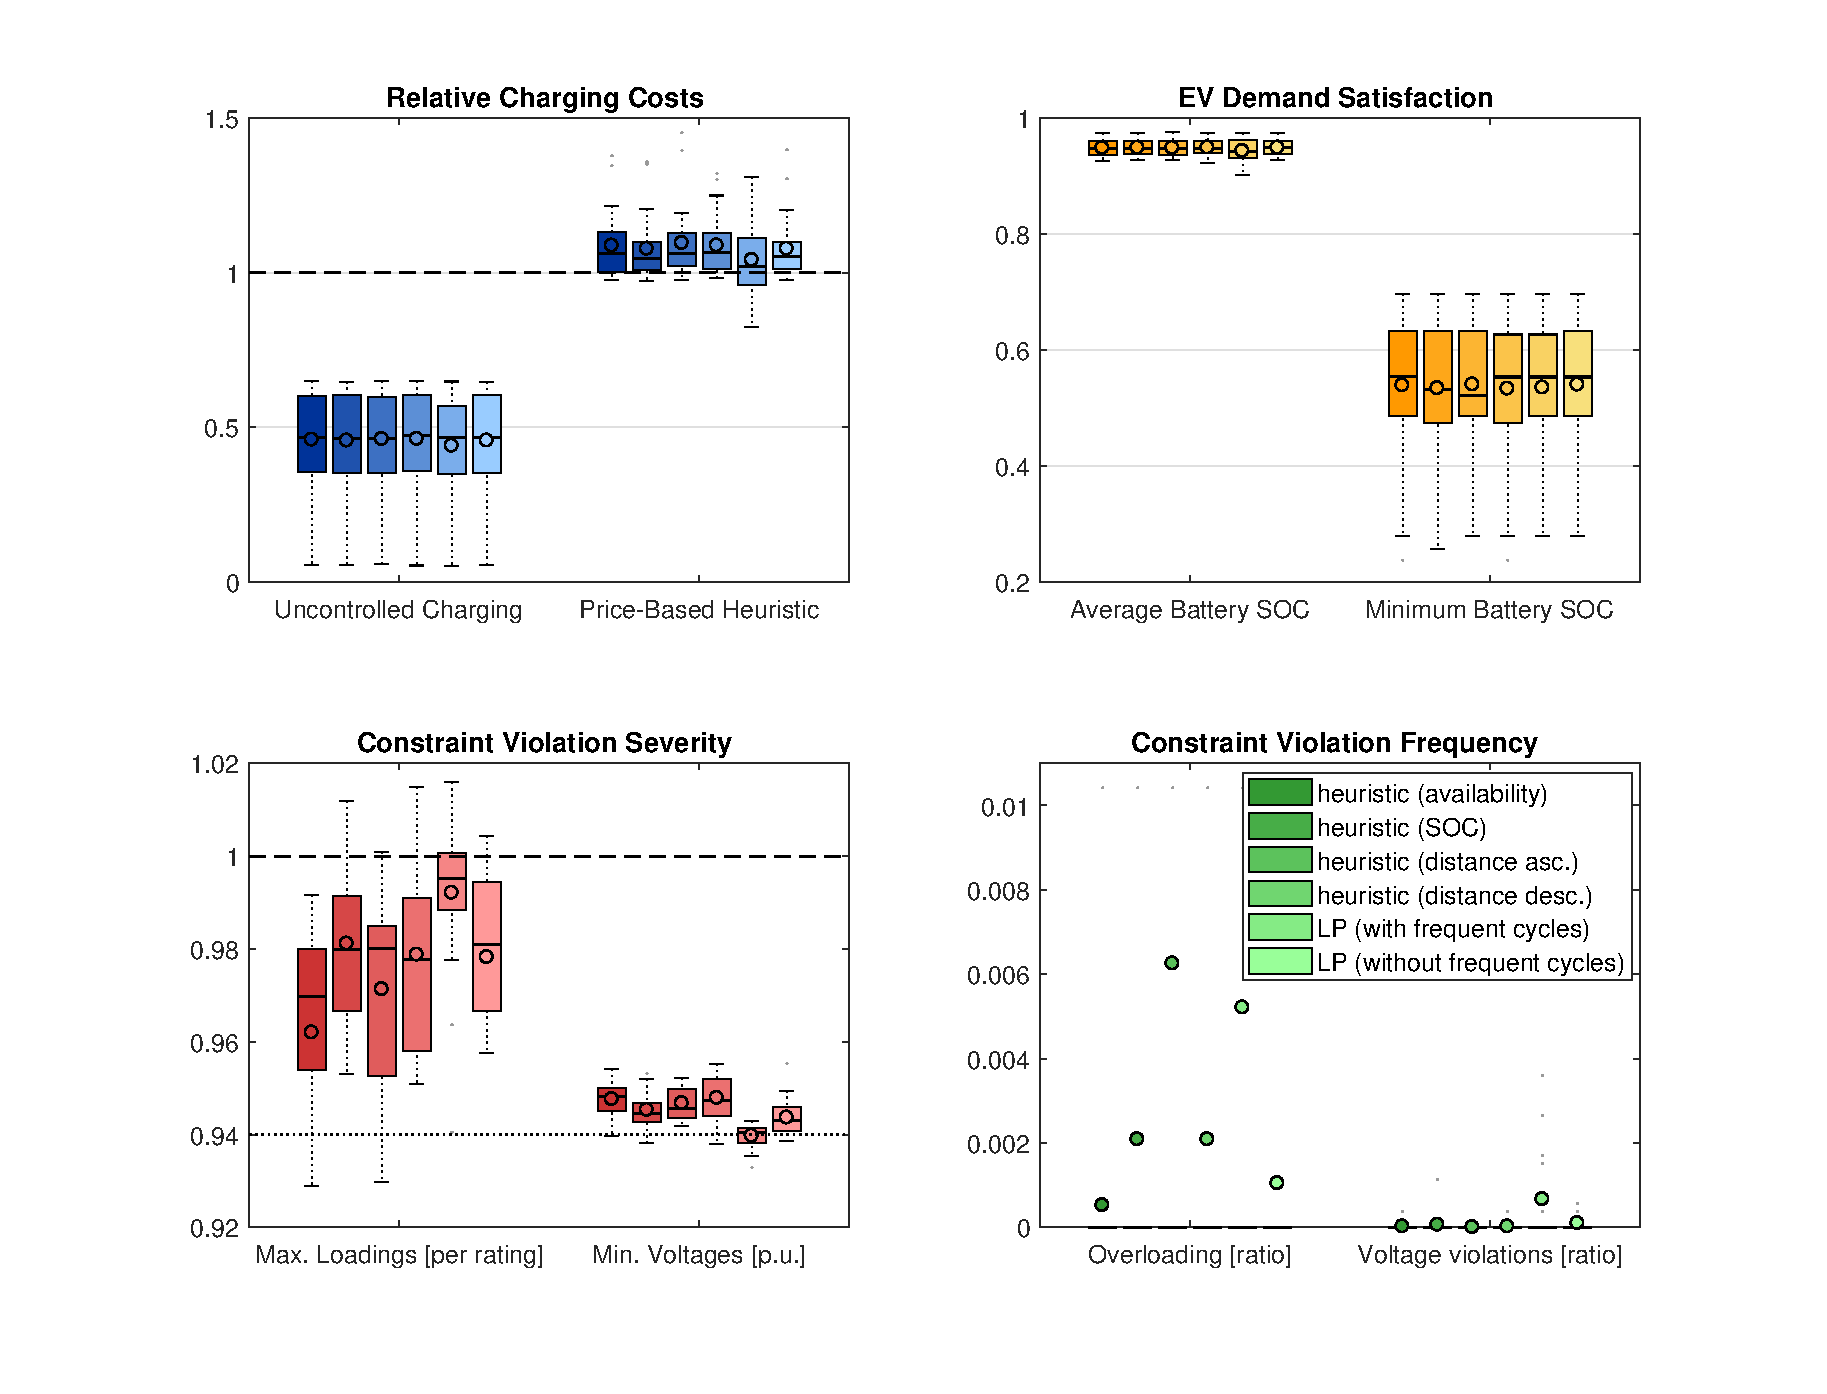
\includegraphics[width=\textwidth,trim={2.9cm 1.5cm 2.5cm 0cm},clip]{figures/evaluation/heulp.eps}
	\caption{Performance of heuristic optimisation modes and linear programming}
	\label{fig:heulp}
\end{figure}

The linear programme (LP) was run in two variants. First, with unconstrained charge rate modulation allowing frequent on/off cycles and, second, with constrained charge rate modulation as prescribed in the constraint formulated in \Autoref{eq:crm} which could not be recognised in heuristic scheduling. The LP allowing frequent cycling achieves another 1.6\% cost reduction compared to uncontrolled charging averaging at 43.99\%, whereas virtually no change in relative charging costs could be observed for the LP including the charge rate modulation constraint. 

However, because the latter obstructs maximum charging rates on the edges of the availability period, but requires slow ramping of charging rates, the average fulfilment ratio of demand stabilises on the niveau of the heuristics, which had deteriorated marginally for the unconstrained LP. Likewise, in the technical domain, the LP with restricted charge rate modulation outperforms its unconstrained pendant. More than half of the analysed scenarios exhibits some voltage violations in the network, whereas this is reduced to a fraction for the constrained LP.

In general, the fact that the cost increase from unconstrained to network-constrained optimisation is confined to the order of 10\% on average is remarkable. Since it was established that the price-based heuristic causes severe slot-wise violations, this indicates that numerous alternative slots with similar charging costs and suitable capacities are available limiting the financial impact of network constraints.

\section{Sensitivity Analysis of Uncertainty Mitigation Approaches}
\label{sec:saunc}

This section analyses the sensitivity of algorithm performance to different parameter configurations of the uncertainty mitigation approaches presented in \Autoref{sec:uncmitigation}. The parameters mirror varying degrees of conservatism and determine the extent of security margins applied. The base case for comparison was chosen to be the LP with constrained charge rate modulation.

\subsection{Vehicle Availability Uncertainty Attenuation}

\Autoref{fig:lpav} reveals a limited effect for availability uncertainty attenuation in non-technical regards: except for a minor improvement in minimum battery charge levels from 54.00\% to 54.83\% on average at negligible extra cost, no refinement could be noted. A reason for the limited effect of availability uncertainty mitigation falling short of expectations is that the slow ramping of charging rates in the LP already mitigates inherently by not allocating maximum charge rates in rather uncertain boundary regions of predicted availability. Nonetheless, this approach constitutes a valuable addition if a charge rate modulation constraint is not imposed. %PROOF!

\begin{figure}[]
	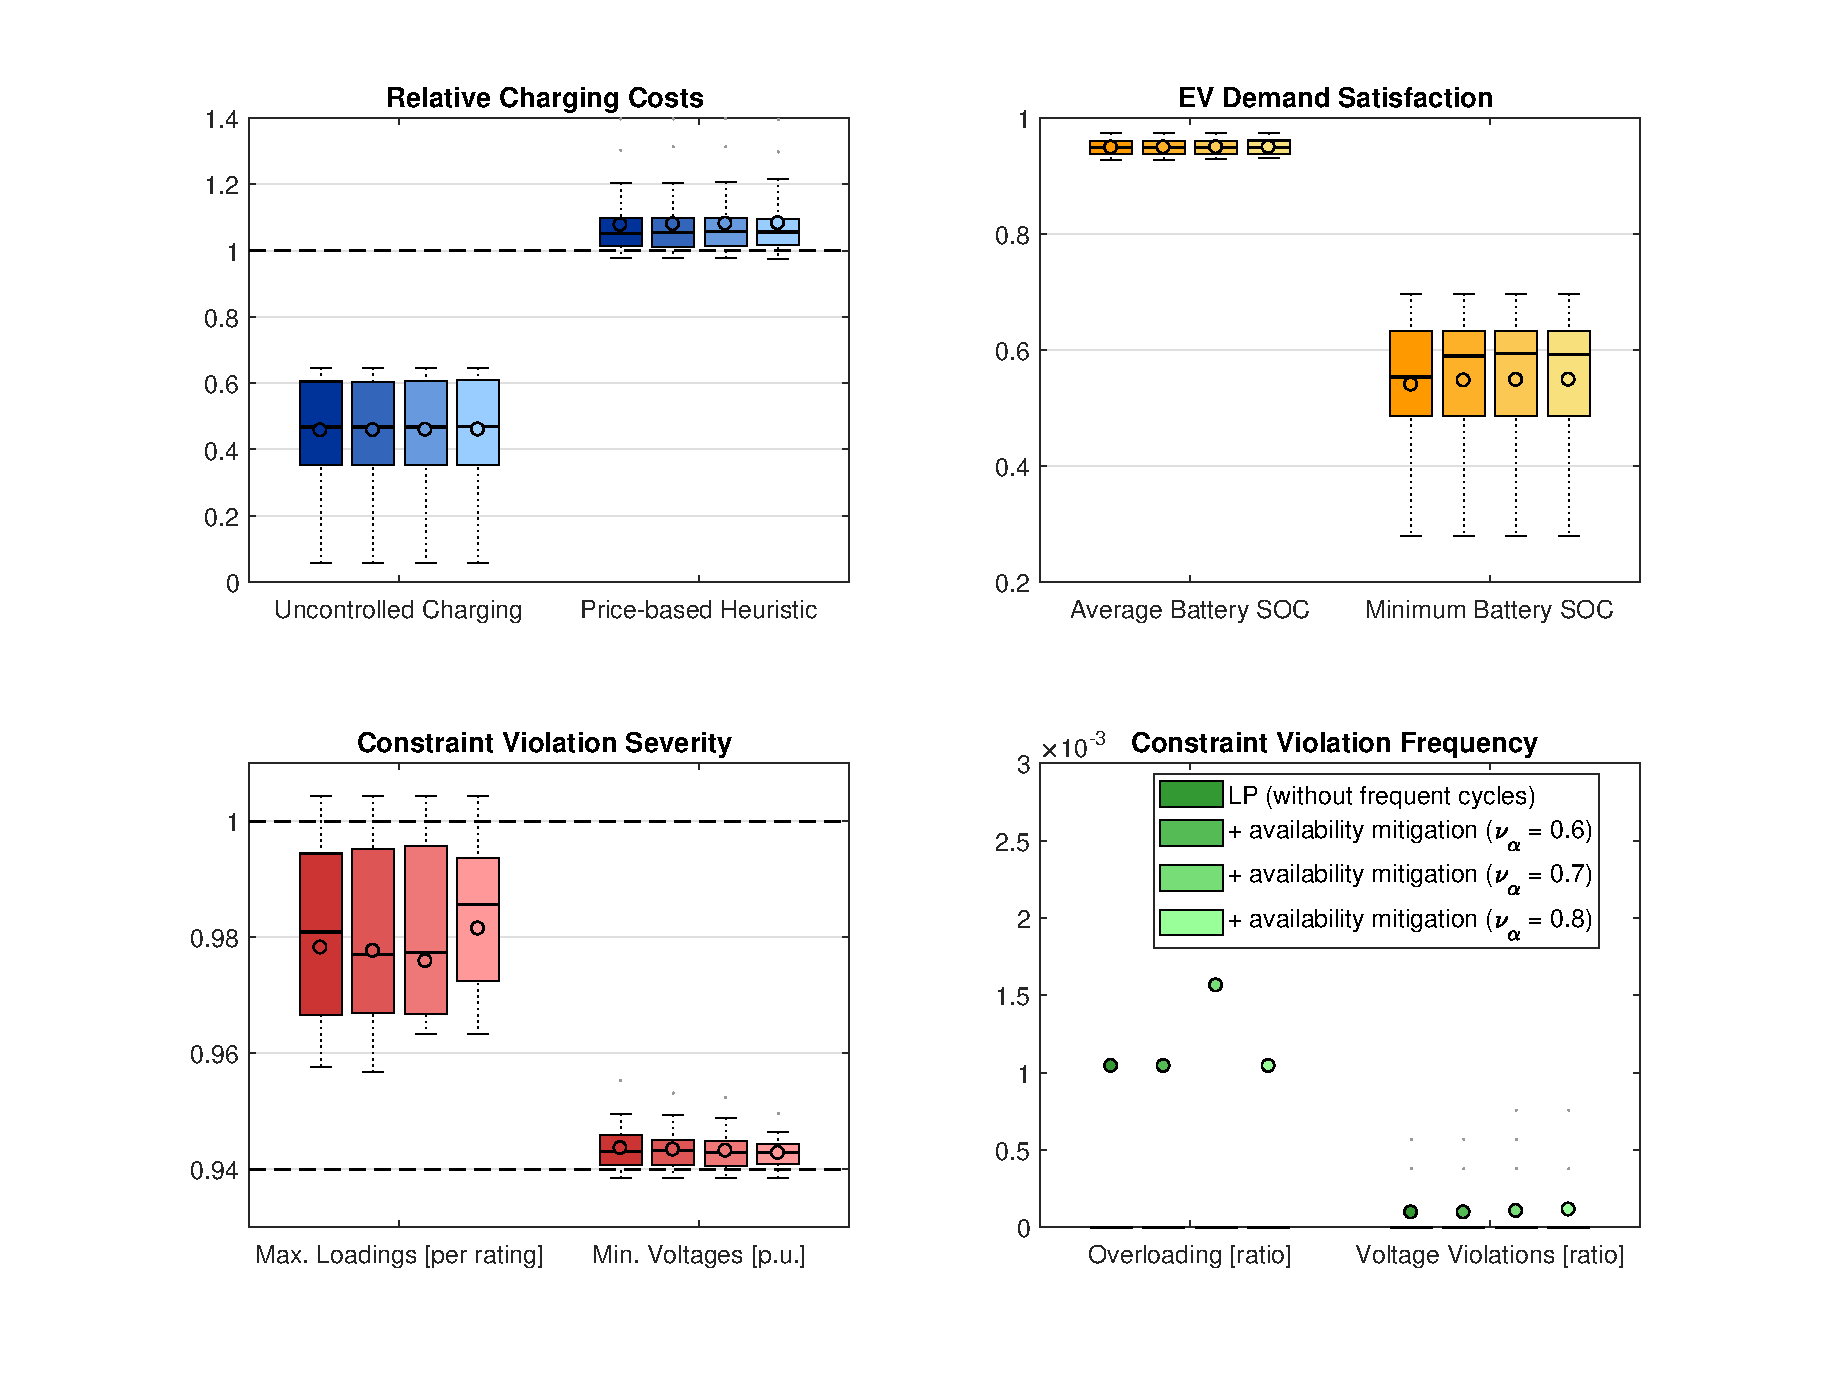
\includegraphics[width=\textwidth,trim={2.9cm 1.5cm 2.5cm 0cm},clip]{figures/evaluation/lp_av.eps}
	\caption{Sensitivities of availability uncertainty mitigation parameters}
	\label{fig:lpav}
\end{figure}

Technically, discernible changes are observed exclusively for high security margins. The average line loading increases, while voltages tend to deteriorate marginally. This effect is induced by the limited load flexibility of electric vehicles due to a high level of conservatism and, thus, constellations in which loads aggregate on fewer slots even if sub-optimal. By subjective weighting, parameter $\nu_{\alpha}=0.6$ is chosen to enter into the joint mitigation parameter set.

\subsection{Battery State of Charge Uncertainty Attenuation}

Battery state of charge uncertainty mitigation summarised in \Autoref{fig:lpsoc} yields results as intuitively expected. With increasing security constraints, while charging costs increase, the reliability of EV demand satisfaction rises; especially the minimum final battery charge increases rapidly. Charging for a battery state of charge that is not lower in 80\% of all cases leads to satisfaction rates of more than 98.18\% on average compared to previously 94.86\% and minimum charge levels of 74.08\% rather than mere 54.00\% for a limited increase in costs of 10\%. Because electric vehicles are scheduled to provide more energy than they are actually expected to require, necessarily some schedule slots will remain unused and may not coincide with the most economical benign slots if simply cut off by a controller once a full charge is reached.

\begin{figure}[]
	\centering
	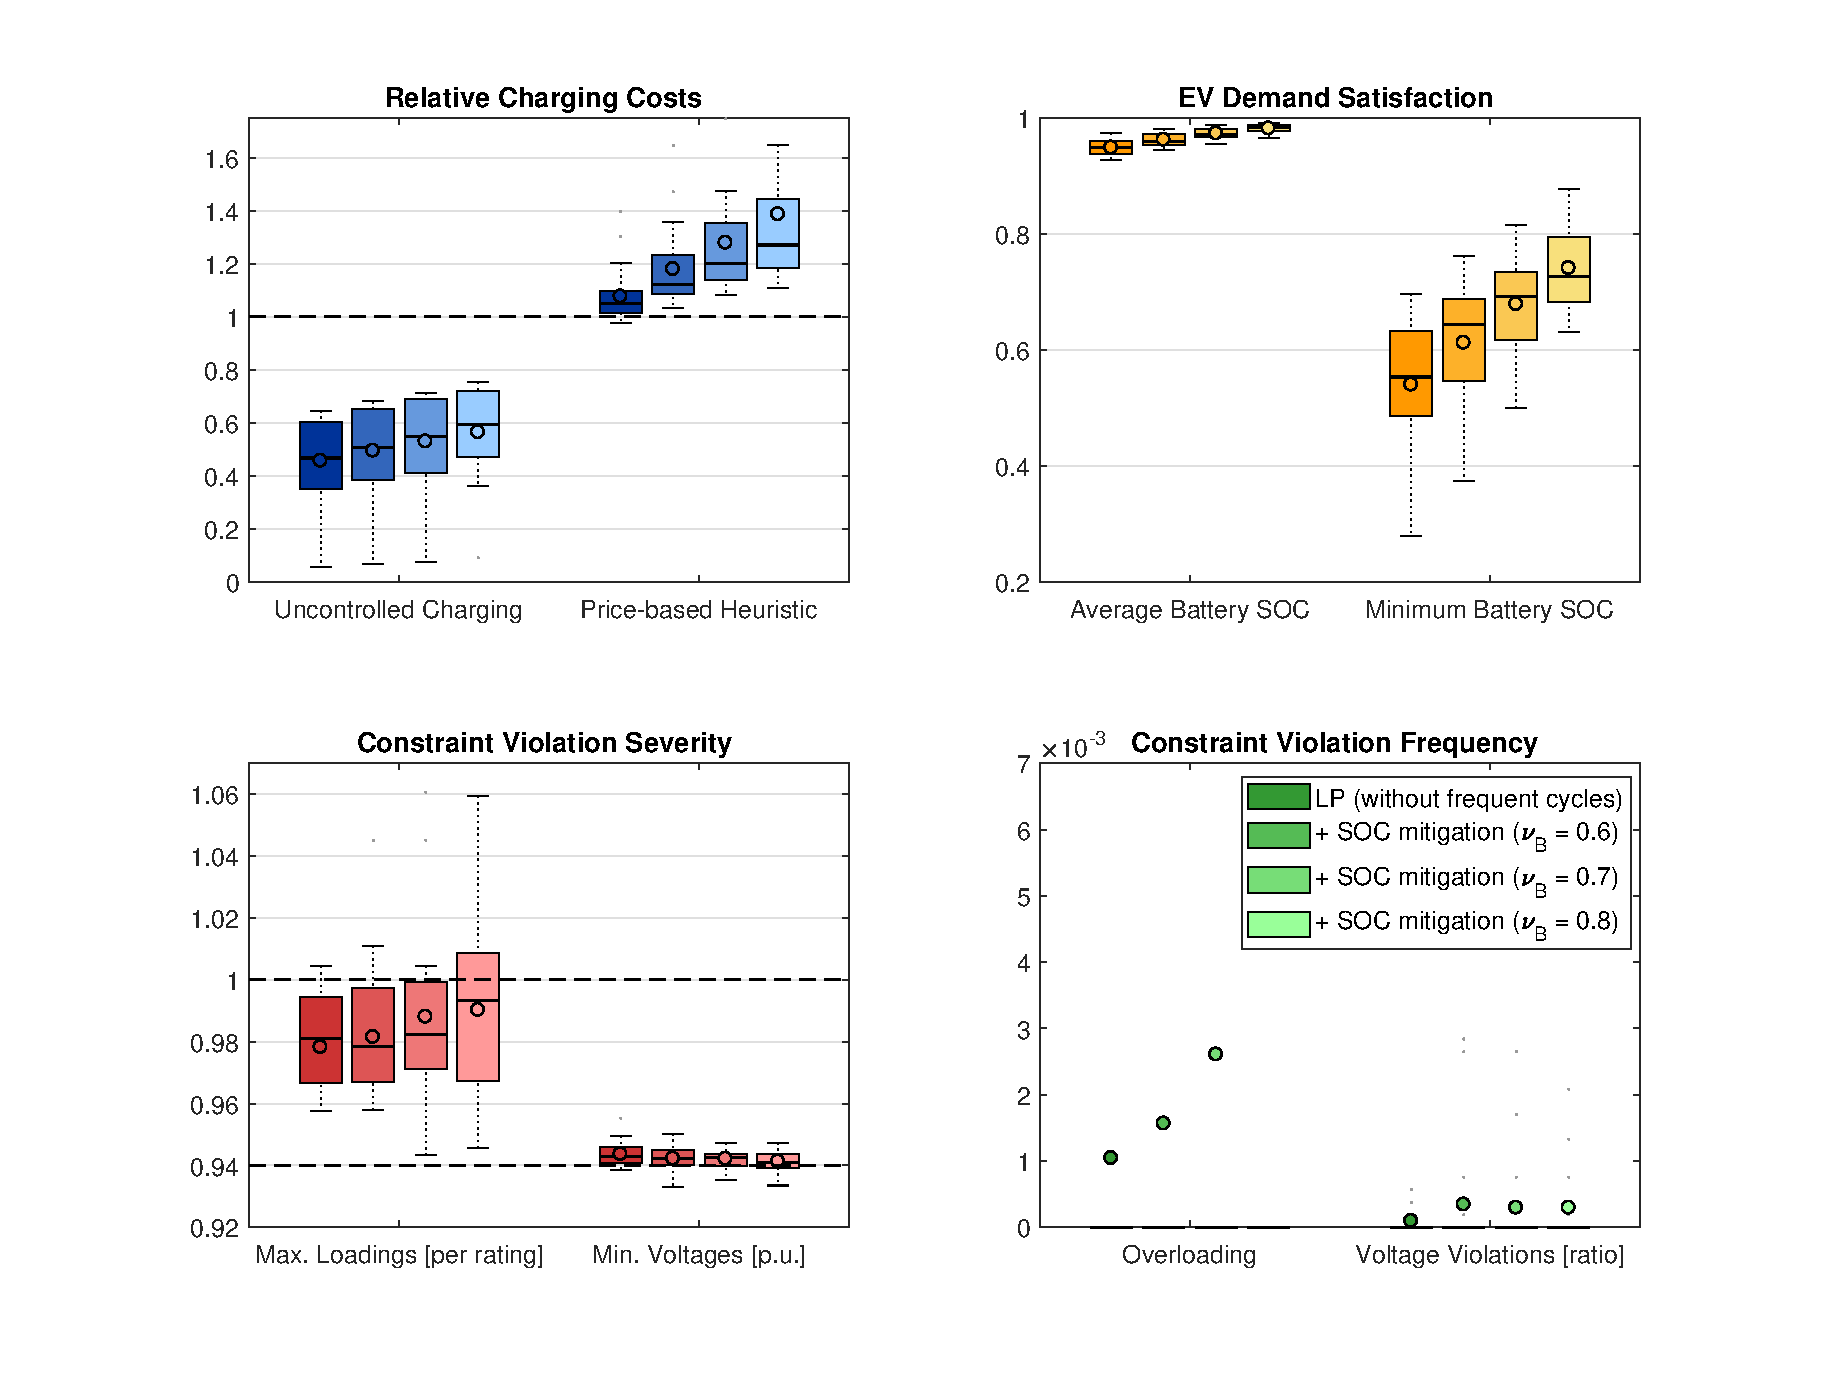
\includegraphics[width=.98\textwidth,trim={2.9cm 1.7cm 2.5cm 0.9cm},clip]{figures/evaluation/lp_soc.eps}
	\caption{Sensitivities of daily mileage uncertainty mitigation parameters}
	\label{fig:lpsoc}
\end{figure}

\newpage
A more intelligent controller might alleviate this price rise by deleting the most expensive redundant slots from the schedule after arrival and knowledge about the battery state of charge is available. Nonetheless, with either type of controller charging will be more expensive as there is a trade-off between granting an electric vehicle flexibility and blocking cheap time slots for others. The unused scheduled charge rates of one electric vehicle could have potentially reduced costs for another and freed network capacity in inexpensive slots stays unexploited. Therefore, the increased satisfaction levels of EVs participating in controlled charging is purchased by a suboptimal allocation of finally realised charging processes.

Moreover, the flexibility through this form of uncertainty mitigation fosters the violation of network constraints as loads must partially be allocated in slots where inhabitants are active, and residential electricity demand is inflicted with more substantial uncertainties. Again, the parameter $\nu_{B}=0.7$ is subjectively chosen for the joint mitigation parameter set. Higher security margins were excluded as these yielded frequent infeasible problem formulations as too much load was demand under given constraints.

\subsection{Market Price Uncertainty Attenuation}

The application of market price uncertainty mitigation is effective at reducing the uncertainty about realised charging costs. \Autoref{fig:lppr} illustrates how the range of deviations of simulated charging costs from the predicted costs of the schedule shrinks with increasing security margins $\nu_{\pi}$. Particularly the step from $\nu_\pi=0.95$ to $\nu_\pi=0.99$ is very effective, which is underlined by the compilation of ranges in \Autoref{tab:costrange}. As this is achieved by shifting the schedules away from the most inexpensive but highly uncertain slots, an average cost increase of 2.34\% from \pounds 44.32 to \pounds 45.35 results. Because of the little distortion of price ranking, for lower $\nu_{\pi}$ the approach is ineffective. In conclusion, efficacy requires alterations in the price ranking.

\begin{figure}[]
	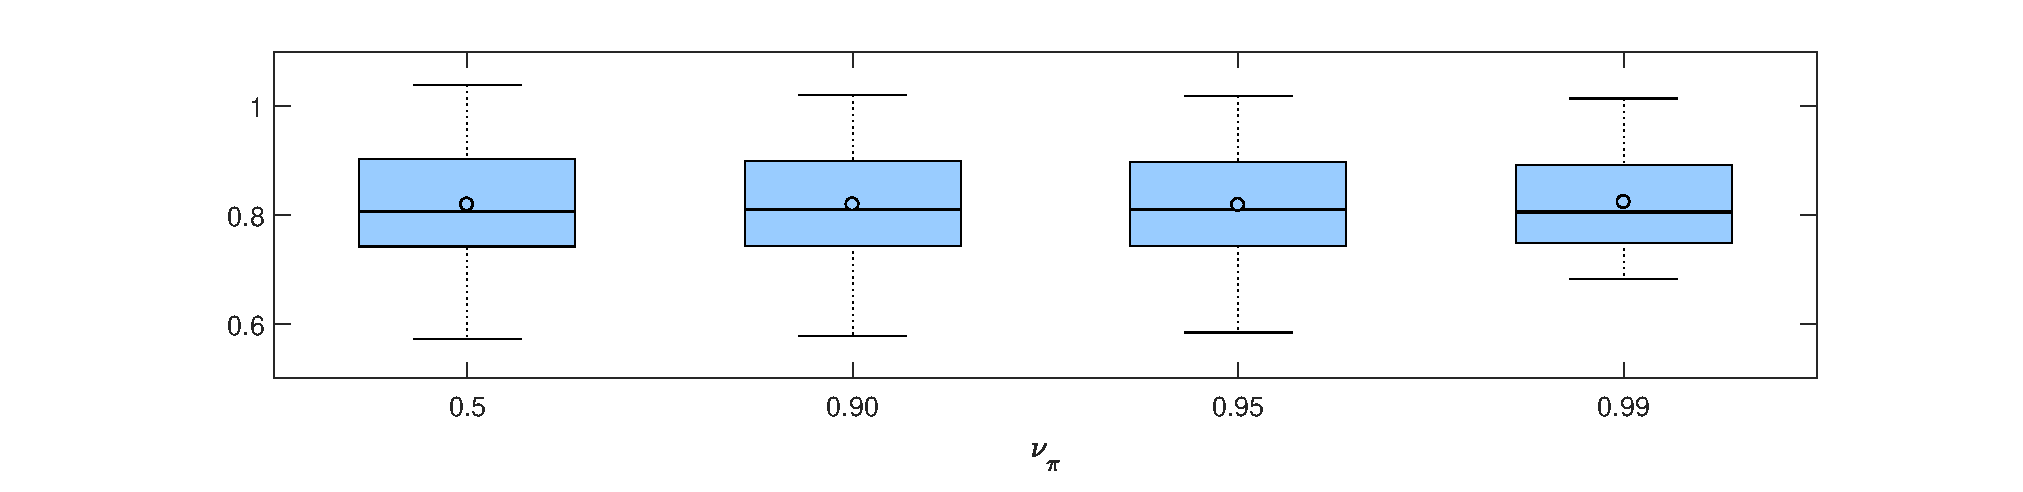
\includegraphics[width=\textwidth,trim={2.9cm 0cm 2.5cm 0cm},clip]{figures/evaluation/lp_pr2.eps}
	\caption[Sensitivity of price uncertainty mitigation parameters]{Simulated costs in relation to predicted costs of schedule with varying price uncertainty mitigation parameters. Shows the sensitivity of price uncertainty mitigation.}
	\label{fig:lppr}
\end{figure}

\begin{table}[]
	\centering
		\begin{tabular}{@{}llllll@{}}
			\toprule
			$\nu_\pi$ & \textbf{0.5}   & \textbf{0.90}   & \textbf{0.95}   & \textbf{0.99}  & \textbf{[unit]} \\ \midrule
			Maximum & 1.039 & 1.020 & 1.019 & 1.014 & - \\
			Minimum & 0.573 & 0.578 & 0.884 & 0.683 & -\\
			Range     & 0.466 & 0.442 & 0.434 & 0.331 &-  \\
			Average simulated costs & 44.32 & 44.43 & 44.43 & 45.35 & \pounds\\ \bottomrule
		\end{tabular}%
	\caption[Sensitivity of price uncertainty mitigation parameters]{Ranges of simulated costs in relation to predicted costs of schedule with varying price uncertainty mitigation parameters. Shows the sensitivity of price uncertainty mitigation.}
	\label{tab:costrange}
\end{table}

\subsection{Residential Demand Uncertainty Attenuation}

With little to no infringement on charging costs or satisfaction of electric vehicle demand, the introduction of a demand mitigation approach with a rolling maximum demand profile recognising a 30-minute window size for residential loads entailed a substantial improvement of the schedules' technical performance as depicted in \Autoref{fig:lpdem}. Both overloads and voltage violations were eliminated in all sampled scenarios. Hence, it constitutes a valuable addition to the EV scheduling approach and will be reflected in the joint mitigation with $w = 0.5$h. Similar to the battery uncertainty mitigation, no larger windows were regarded as these would engender intrinsic overloads and voltage violations even without the presence of EVs and grant no possibility to accommodate EV loads in remaining network capacity.

\begin{figure}[]
	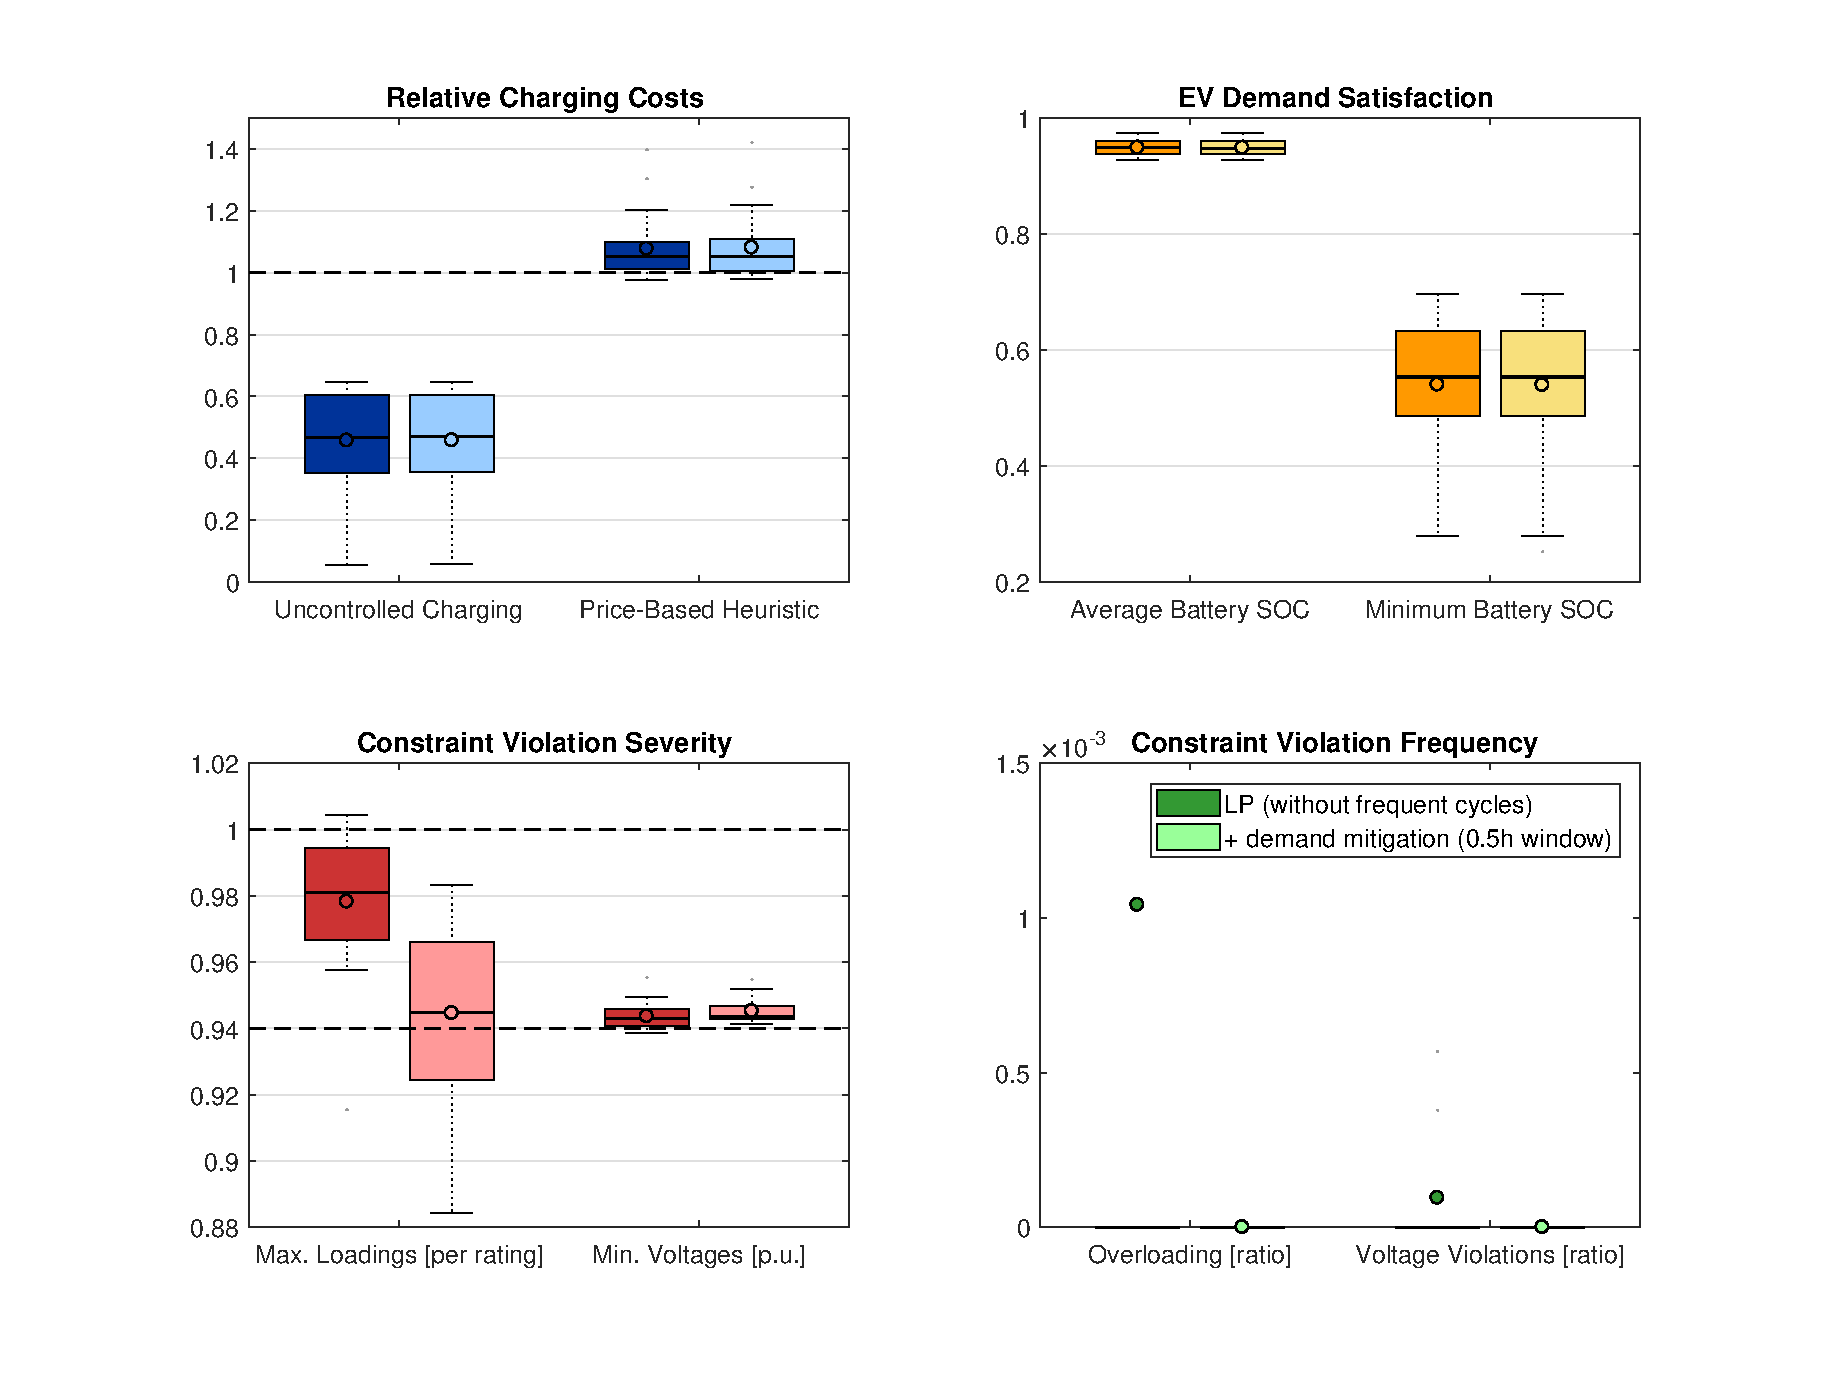
\includegraphics[width=.98\textwidth,trim={2.9cm 1.7cm 2.5cm 0.9cm},clip]{figures/evaluation/lp_dem.eps}
	\caption{Sensitivities of demand uncertainty mitigation parameters}
	\label{fig:lpdem}
\end{figure}

\subsection{Joint Uncertainty Attenuation}
\label{sec:joint}

Individual uncertainty mitigation options have shown that benefits can be drawn to varying degrees. Recall that adapting demand and battery charge level parameters have shown most improvements. It is, however, also vital to evaluate the EV scheduling optimisation, when multiple mitigation approaches are applied simultaneously. As previously noted, too extreme degrees of conservatism may obstruct the feasibility of the problem formulation. Jointly applying security margins to multiple uncertain input parameters bear the potential to be prohibitive and, therefore, are put in a broader perspective via a comparison to the best heuristic and the two LP variants as summarised in \Autoref{fig:joint}.

Indeed, the joint uncertainty mitigation serves its purposes and is generally feasible for the selected subset of parameters. First, the fulfilment ratio of both minimum and average demand could be enhanced to 68.57\% and 97.37\% respectively. Second, neither do voltage violations occur nor are thermal line ratings exceeded. Whether the advantage in EV demand satisfaction on the customer side and the observation of network constraints on the distribution system operator side are worth the reduced cost savings in the order of 10\% in comparison to uncontrolled charging could be based on a willingness to pay or, more accurately, get paid approach. By surveying EV owners the value of a conceivable compensation paid by the aggregator for not completely charging the corresponding battery is determined. Likewise, the inclination of the distribution network operator to appreciate the robustness of the adapted EV schedules depends on the DNO's toolbox, i.e.\ what are its alternative means to overcome unplanned voltage drops or excess demand in the network and what are their respective operating cost. Both considerations are pivotal for the real implementation of the scheduling method but require rigorous analysis of another domain. Instead, this work focusses on what the cost is and eludes a recommendation whether the increase in costs is economically justified.

\begin{figure}[]
	\centering
	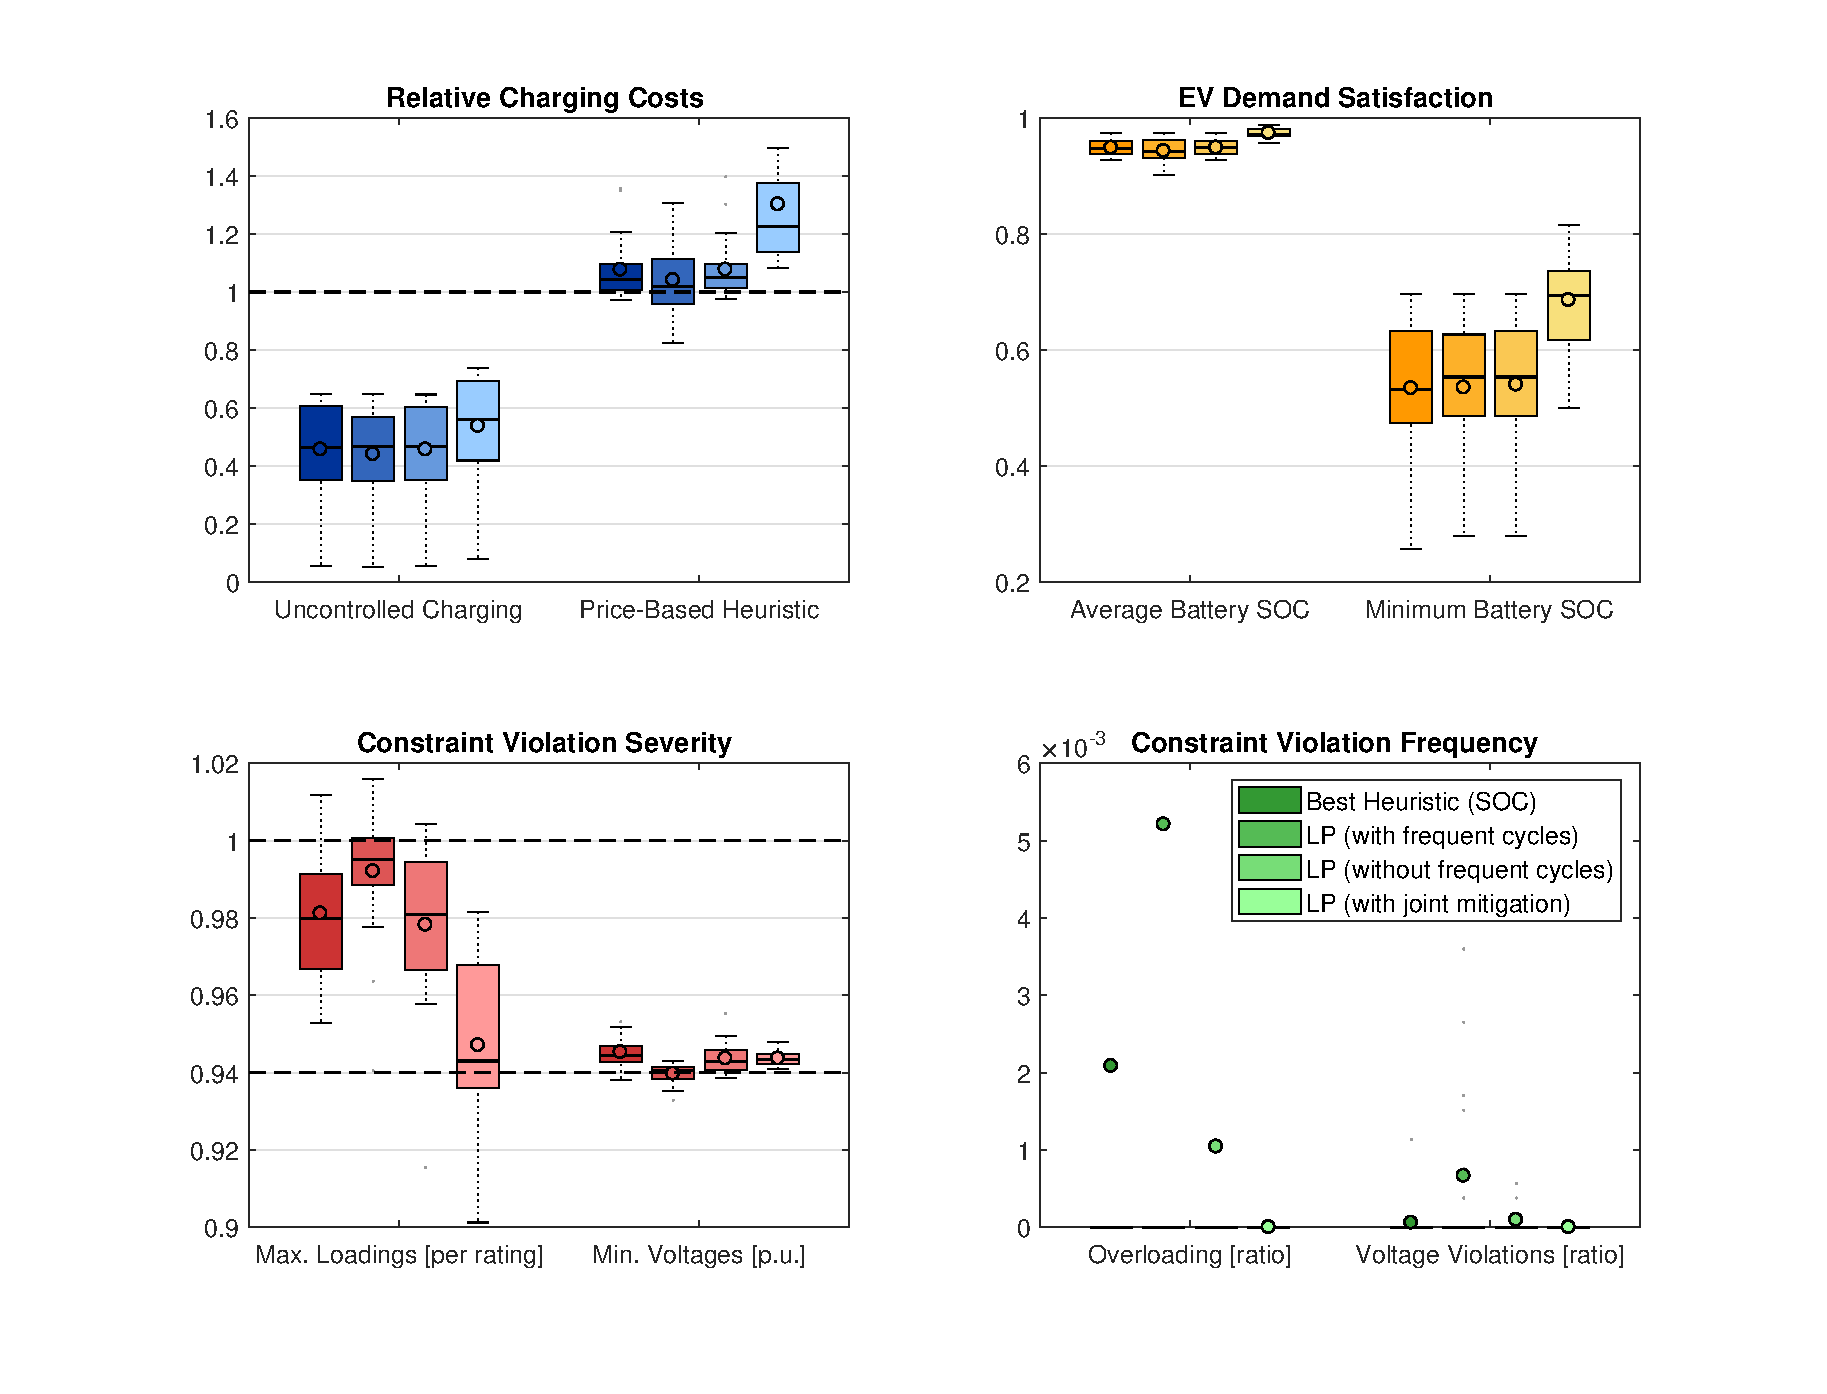
\includegraphics[width=0.98\textwidth,trim={2.9cm 1.7cm 2.5cm 0.9cm},clip]{figures/evaluation/joint.eps}
	\caption{Performance benchmark of joint uncertainty mitigation with linear programming}
	\label{fig:joint}
\end{figure}

%\vspace{-18pt}
\section{Scenario-Level Evaluation}
\label{sec:sceneval}

So far focus was put on the overall performance of different scheduling approaches across scenarios. This section is dedicated to an exemplary scenario for an in-depth study of the lost potential due to the presence of uncertainty and how schedules differ when uncertainty mitigation is applied. Therefore, \Autoref{fig:99} overlays the reference case analysis of \Autoref{fig:dumbprice} with LP results without uncertainty mitigation, with uncertainty mitigation, and ultimately an LP given perfect information about its input parameters.

\begin{figure}[]
	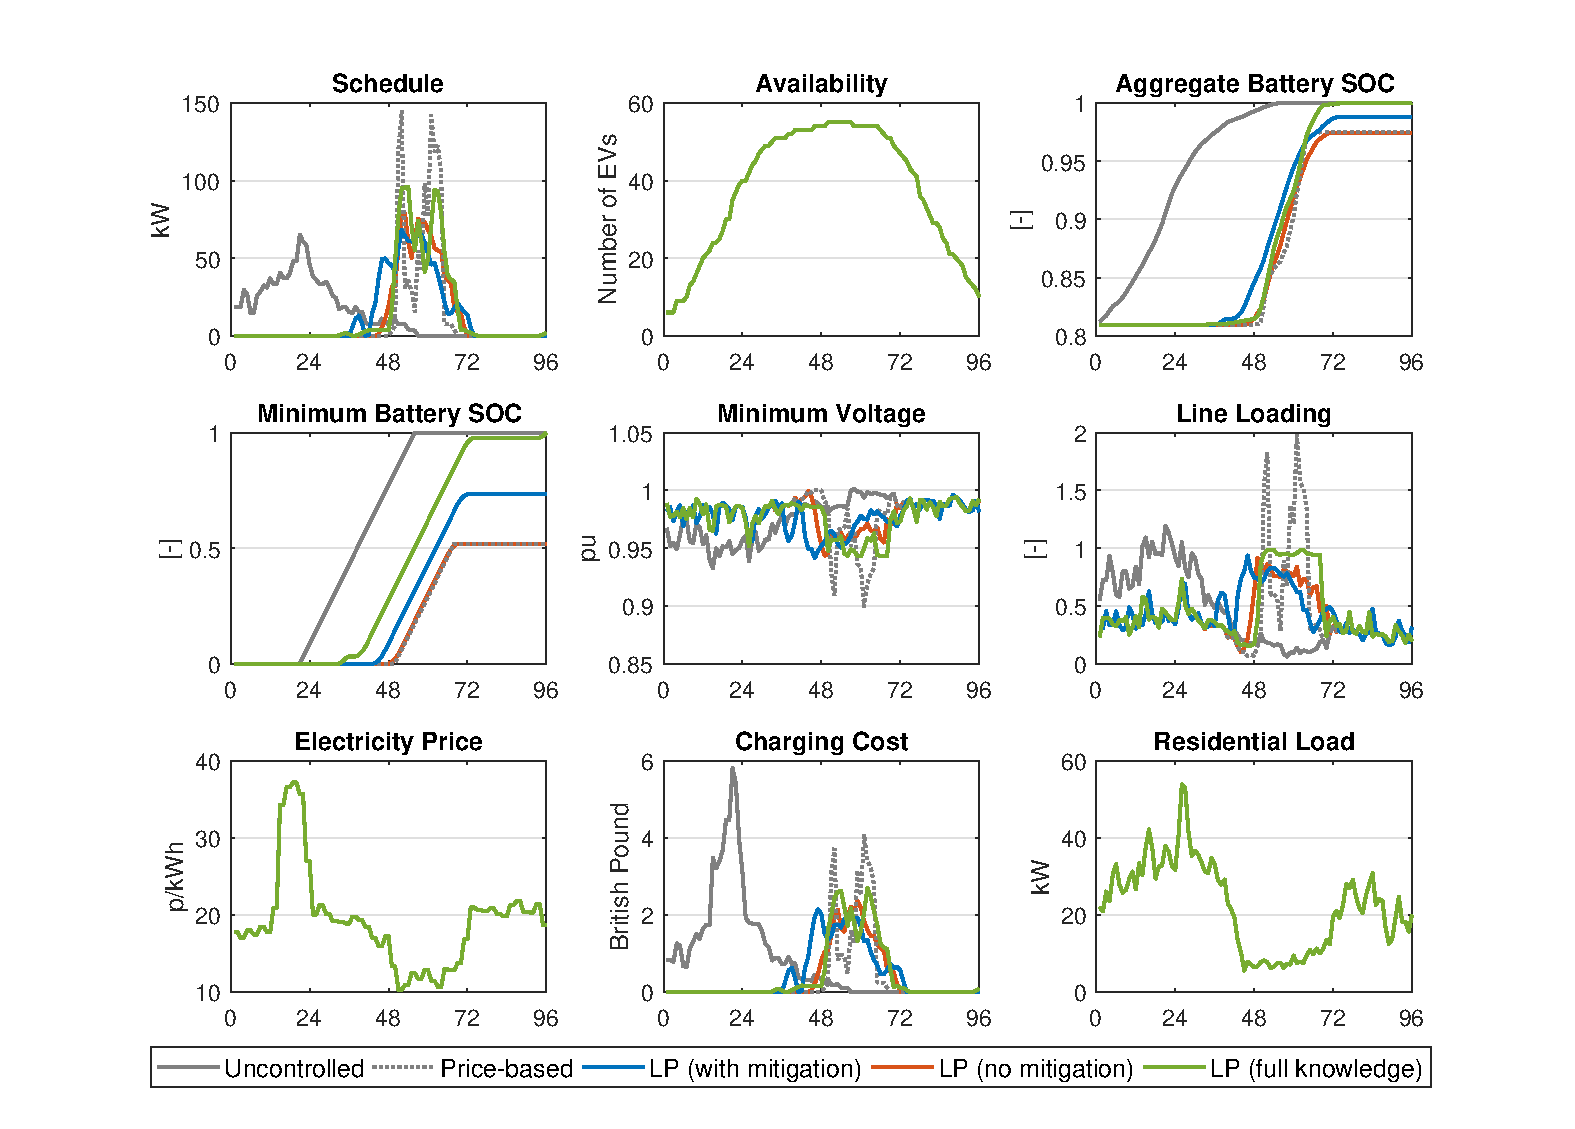
\includegraphics[width=\textwidth,trim={2cm 0cm 1.5cm 0cm},clip]{figures/evaluation/scen/99.eps}
	\caption{Comparison of linear programming with/without uncertainty mitigation}
	\label{fig:99}
\end{figure}

Clearly, loads tend to be allocated in slots with low electricity prices and high chances of availability. Moreover, they concentrate on periods of low residential demand limiting the impact of demand uncertainty and allowing substantial EV loads to be allotted in these slots. By comparison also in this specific scenario demand satisfaction is improved by uncertainty mitigation. This is achieved by increasing the scheduled energy for all EVs. Because the simple controller starts with the earliest scheduled slots and cuts off once the battery is fully charged, the resulting aggregate charge curve is shifted to earlier time slots and some of the cheapest slots are less exploited.

\begin{figure}[]
	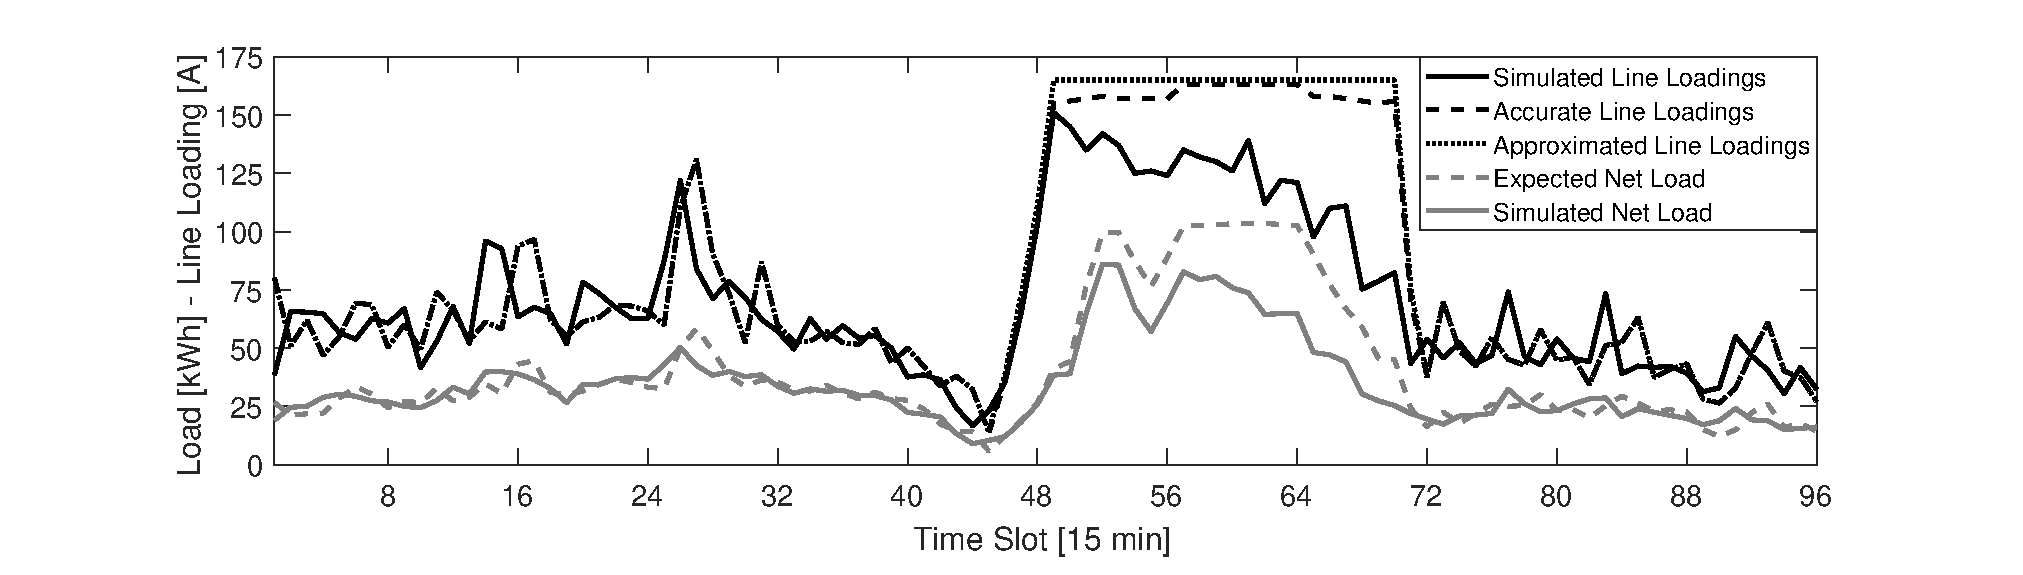
\includegraphics[width=\textwidth,trim={2cm 0.0cm 1.5cm 0cm},clip]{figures/evaluation/scen/constraints.eps}
	\caption{Constraint observation and reasons for the lack of capacity utilisation}
	\label{fig:constraints}
\end{figure}

Moreover, both LP variants lack a full capacity exploitation, the cause of which is presented in \Autoref{fig:constraints}. Approximated line loadings only play a minor role in underestimating the actual line loadings. Much more it is the net load falling short of expectations leading to a limited loading of the mains cable in inexpensive slots. A look at the LP run with perfect information supports that high rates of capacity exploitation are possible and deviations are due to prediction errors. It could further be noted that both voltage constraints, as well as maximum line loadings, take turns at causing a limitation of charging powers in respective slots.

\subsubsection*{Variation of optimal schedules due to uncertainty mitigation}

While the change in aggregate EV loads due to uncertainty mitigation was discernible from \Autoref{fig:99}, it is of further interest to examine how the schedules vary on a disaggregated level as depicted in \Autoref{fig:schedule_comparison}. First, the total charging demand increased through the lower assumed initial battery charge levels. This leads to some loads diverging from the cheapest slots. Interestingly, loads at the end of the feeder spread out more for the network is more sensitive to loads at these households. Demand uncertainty mitigation is particularly important for new charging times as they coincide more with times when residents are active. Due to its subtlety diversion from uncertain inexpensive slots cannot be observed. Further minor conceivable changes may occur through a simple exchange of charging times and rates.

\begin{figure}[]
	\centering
	\subfloat[Schedule without uncertainty mitigation]{
		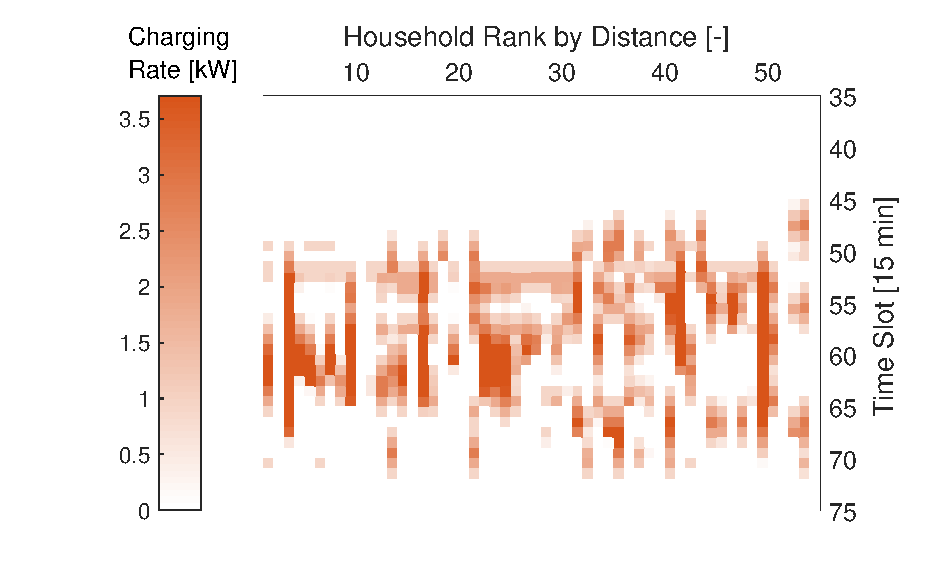
\includegraphics[width=0.48\textwidth,trim={0.2cm 0cm 0.2cm 0cm},clip]{figures/evaluation/scen/sched_nomit.eps}
		\label{fig:schednomit}
	}
	\hfill
	\subfloat[Schedule with uncertainty mitigation]{
		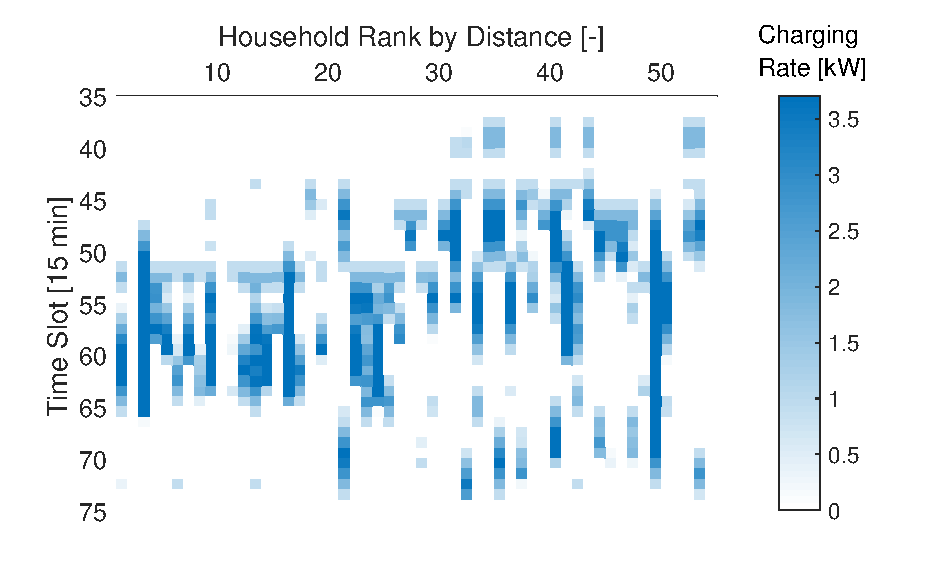
\includegraphics[width=0.48\textwidth,trim={0.2cm 0cm 0.2cm 0cm},clip]{figures/evaluation/scen/sched_mit.eps}
		\label{fig:schedmit}
	}
	\hfill
	\subfloat[Differences in schedules with and without uncertainty mitigation]{
		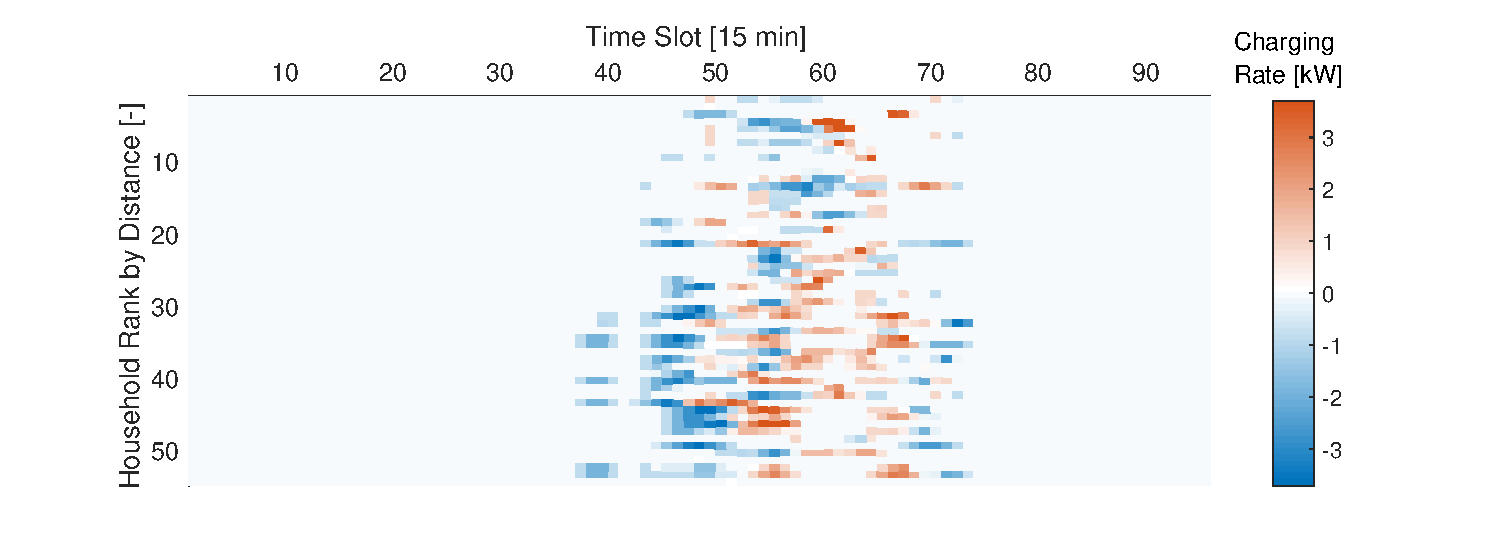
\includegraphics[width=0.95\textwidth,trim={1.5cm 0cm 2cm 0cm},clip]{figures/evaluation/scen/sched_comp.eps}
		\label{fig:schedcomp}
	}
	\caption{Optimal schedule variation due to uncertainty mitigation}
	\label{fig:schedule_comparison}
\end{figure}

\subsubsection*{Further technical issues: load losses and phase balance}

Phase imbalances have been reported to intensify in three-phase low-voltage distribution networks in the presence of electric vehicles \cite{Ul-Haq2015}. Networks are designed for loads balanced across the three phases, where currents in each phase and voltages are approximately equal. Imbalances may result in currents within the neutral line, which tends not to be rated for such currents and may lead to excessive heating \cite{Bass2013a}. This results in an increased risk of failures increases energy losses and may cause significant degradation of power quality \cite{Sun2015} as load imbalances likely entail voltage unbalances, which are in turn problematic for three-phase loads. Indeed, \Autoref{fig:phasebalance} reveals more uneven strains of individual phases for coordinated charging than for uncontrolled charging. In extreme cases, one phase is loaded less than 10 percent while others dominate with a share of more than 60 percent. Multiple means to avoid phase imbalances exist, one of which is to incorporate a phase balance constraint into the EV scheduling problem \cite{Putrus2009,Sun2015}. % FUTURE WORK

\begin{figure}[]
	\centering
	\subfloat[Uncontrolled Charging]{
		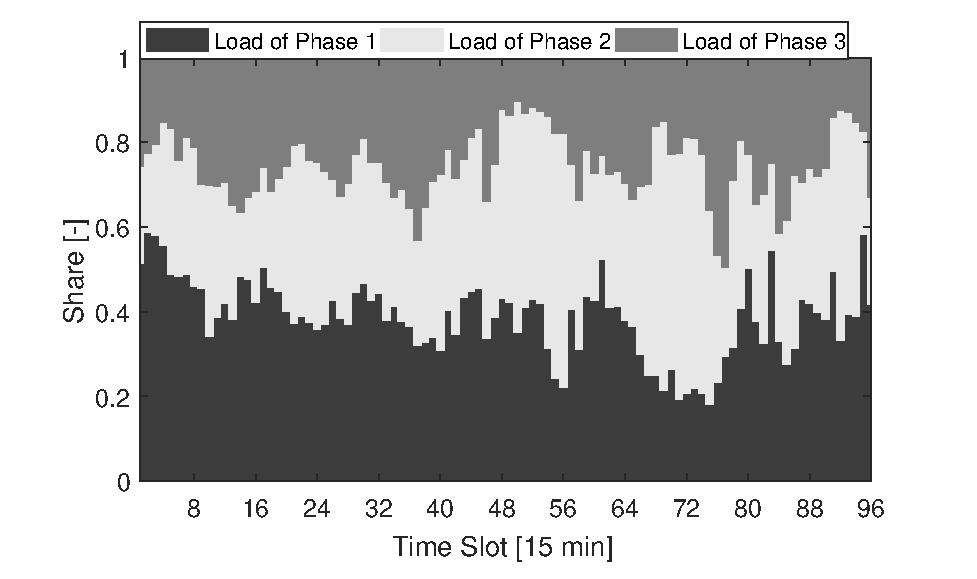
\includegraphics[width=0.48\textwidth,trim={1cm 0cm 1cm 0cm},clip]{figures/evaluation/scen/phasebalance_uc.eps}
		\label{fig:pb_uc}
	}
	\hfill
	\subfloat[LP (with uncertainty mitigation)]{
		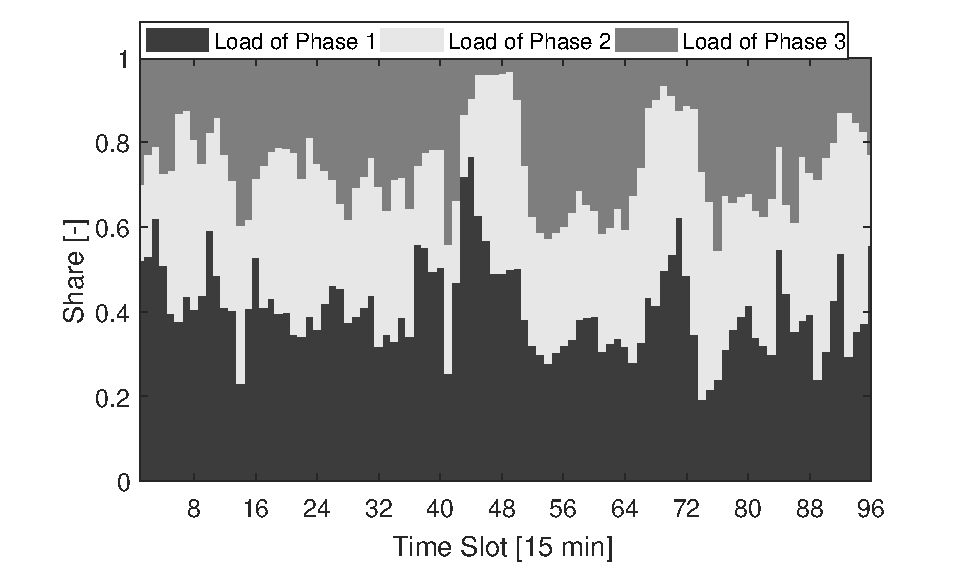
\includegraphics[width=0.48\textwidth,trim={1cm 0cm 1cm 0cm},clip]{figures/evaluation/scen/phasebalance_lp.eps}
		\label{fig:pb_lp}
	}
	\caption{Phase balance of net loads over time}
	\label{fig:phasebalance}
\end{figure}

Another concern is increased losses induced by EV scheduling. \Autoref{fig:loss} depicts load losses following the aggregate residential electricity demand including EVs. The charging rates both affect active and reactive power losses. Noteworthily, while maintaining losses in the range of less than 1\% of the total net load, the LP with uncertainty mitigation leads to an 8\% increase in losses. Hence similar to phase imbalances, the minimisation of losses may be a suitable additional objective for EV scheduling. In fact, loss minimisation has successfully been considered with regards to the limitation of EV impact on power system performance \cite{Sortomme2011, Clement2010,Deilami2011, Fazelpour2014}. However, the studies are confined to the technical optimisation and do not relate the economic benefit to the cost savings which could be obtained from price-based charging.

\begin{figure}[]
	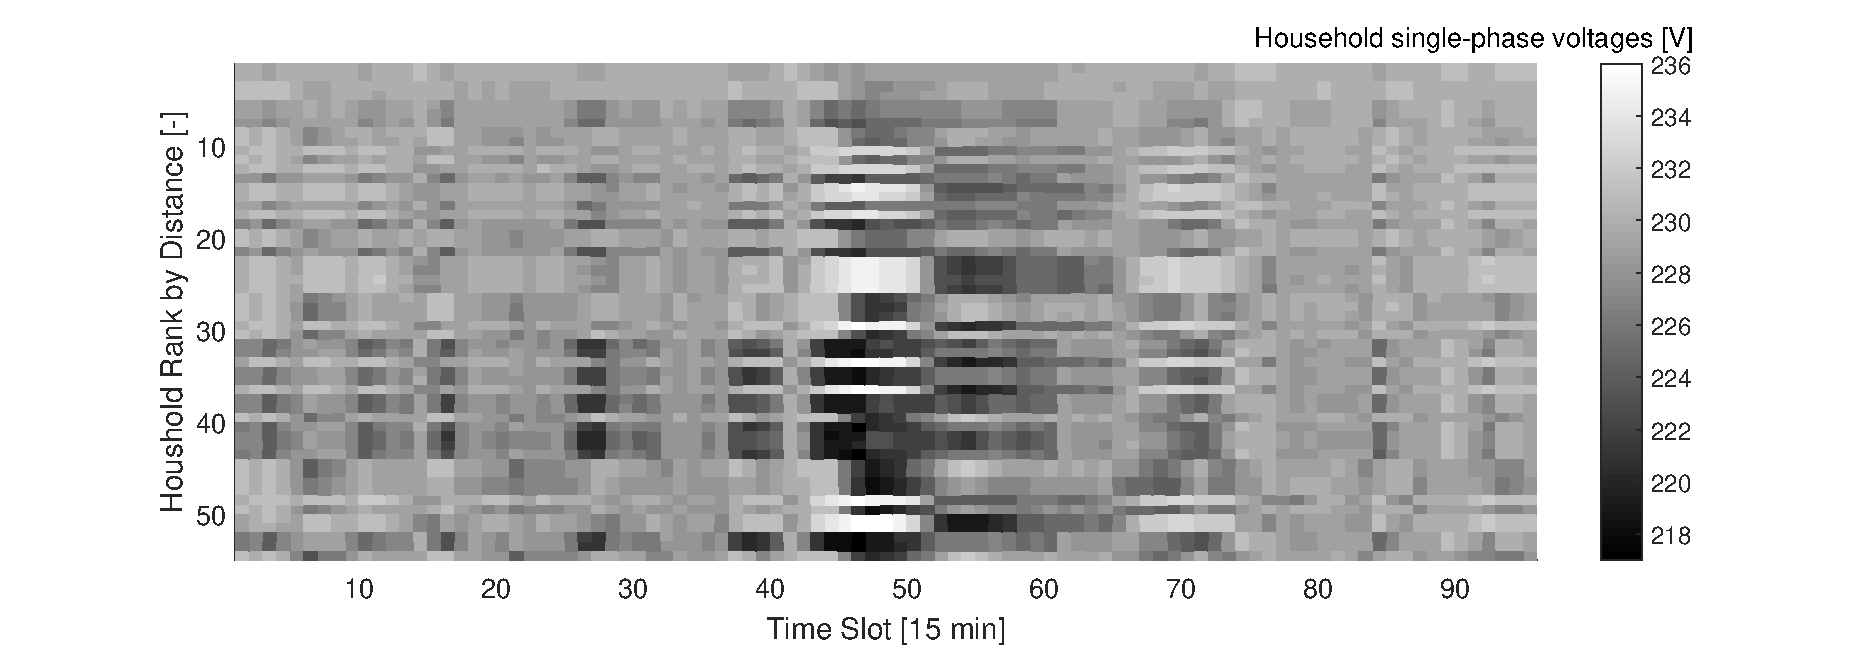
\includegraphics[width=\textwidth,trim={2cm 0cm 2cm 0cm},clip]{figures/evaluation/scen/volts.eps}
	\label{fig:volts}
	\caption{Household voltage temporal and spatial distributions (LP with uncertainty mitigation)}
\end{figure}

\begin{figure}[]
	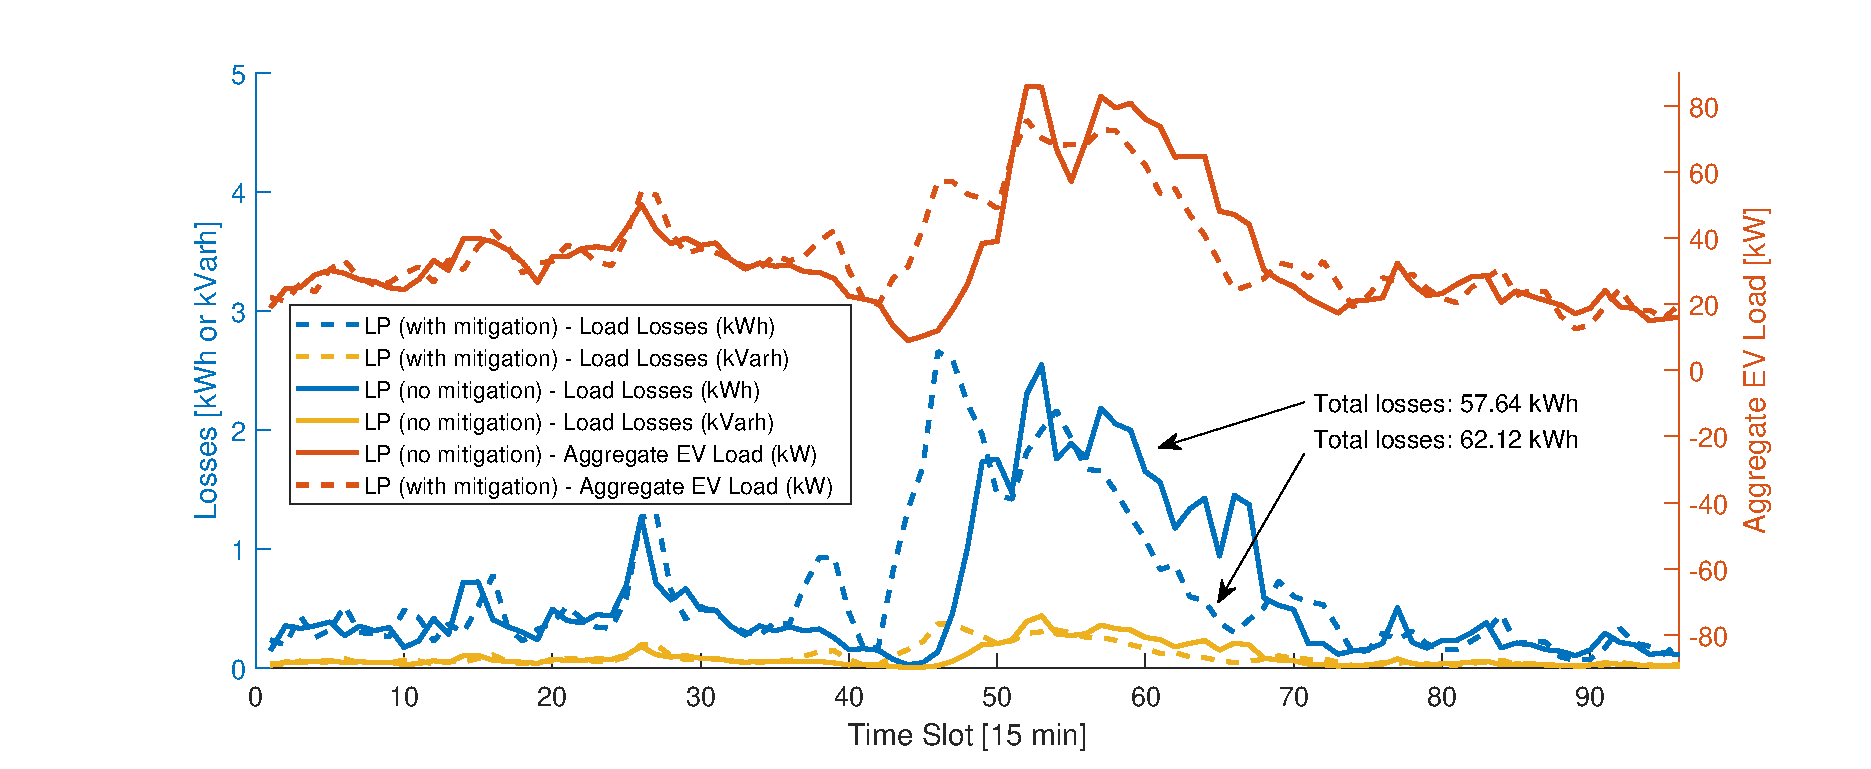
\includegraphics[width=\textwidth,trim={2cm 0cm 2cm 0.7cm},clip]{figures/evaluation/scen/losses.eps}
	\caption{Load losses in relation to aggregate EV loads}
	\label{fig:loss}
\end{figure}

\subsubsection*{Intra-scenario parameter and performance measure distributions}

Looking at the scenario parameters and selected evaluation criteria from a different angle as displayed in \Autoref{fig:hists} provides a more detailed insight into the spread achieved costs and demand satisfaction levels.

First, electricity prices range between \mbox{10-40 p/kWh} and a significant portion of prices remains below \mbox{22 p/kWh}. Because uncontrolled charging does not react to prices, average costs per household are broadly spread under the premise that consumers pay adapted wholesale prices rather than single-rate tariffs. Individual arrival times and the amount of required charge are the exclusive determinants. In comparison to the distribution of electricity prices, the histogram underlines that charging concentrates on peak demand periods with high electricity prices. Inversely, the LP without uncertainty mitigation succeeds at focussing EV loads on inexpensive and draws energy for predominantly less than \mbox{13 p/kWh} and no more than \mbox{19 p/kWh}. Thus, the cost range within which EVs are charged is small. Loads can be allocated in slots of similar prices. This changes when security constraints are applied since it causes a more even distribution of costs ranging between 10 and \mbox{19 p/kWh}. Consequently, the cost of charging is higher for some households than for others, which raises concerns about the redistribution of charging costs by the aggregator.

Second, the distributions of availability periods show that a vast majority of households are available for charging more than 12 hours per day. Coupled with the high initial battery charge levels, where a majority did not use more than 20\% of the stored energy, this exposes the high degree of flexibility of EV loads.

Third, despite the high level of freedom, not all EVs will recharge completely due to prediction errors. For both LP variants, only individual EVs could not be supplied with demanded energy due to heavy deviations from behaviour predictions, i.e.\ vehicles were available only for an insufficient time or had a shallow initial battery charge level. However, the LP with uncertainty mitigation could lift final battery charge levels from the interval $[0.9,0.95]$ to the next $[0.95,1.0]$ affecting around 10\% of vehicles.

\begin{figure}[]
	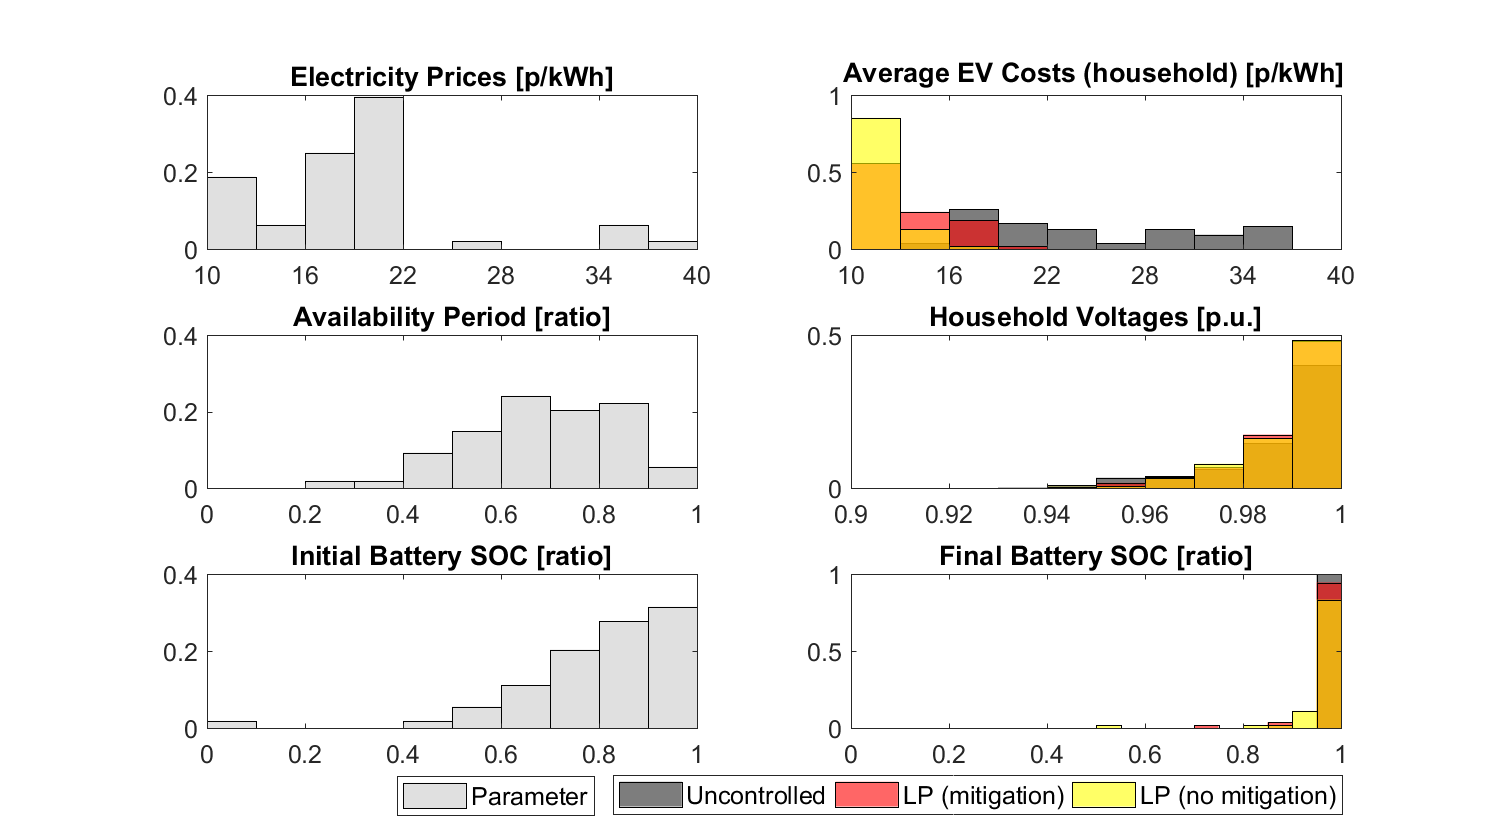
\includegraphics[width=0.9\textwidth,trim={1cm 0cm 1cm 0.5cm},clip]{figures/evaluation/scen/hists.eps}
	\caption{Histograms of scenario parameters and selected evaluation criteria}
	\label{fig:hists}
\end{figure}

\section{Household-Level Evaluation}
\label{sec:hdeval}

To complement the scenario-level evaluation, two exemplary households were picked to gain insight into the implication of EV scheduling to individual households with regards to their point of connection, the uncertainty involved and functioning principle of the controller. 

\begin{figure}[]
	\centering
	\subfloat[Household 17 (close to substation)]{
		\includegraphics[width=0.48\textwidth]{figures/evaluation/ind/ind17.eps}
		\label{fig:ind17}
	}
	\hfill
	\subfloat[Household 54 (far from substation)]{
		\includegraphics[width=0.48\textwidth]{figures/evaluation/ind/ind54.eps}
		\label{fig:ind54}
	}
	\caption{Household-level effect of point of connection, uncertainty, and controller}
	\label{fig:examplehds}
\end{figure}

\Autoref{fig:ind17} shows the characteristics of a home close to the substation. It generally exhibits high bus voltages, which are weakest when EV charges locally. Overall, voltages tend to weaken when the price is low, and EV loads are allocated elsewhere. Periods, where the electric vehicle is available, are shaded. It becomes apparent that the day-ahead schedule failed to predict the availability period correctly. Due to low prices, the vehicle was scheduled to charge in a period where availability was predicted. However, because the vehicle departed earlier than expected and planned charging processes are missed, the battery could not be refilled completely.

Conversely, \Autoref{fig:ind54} shows the features of a household located further away from the transformer. Lower voltages persist throughout the optimisation horizon, but similarly, voltages are weakest when the corresponding vehicle is charged, and lower voltages coincide either with peak residential demand or EV loads elsewhere prompted by low electricity prices. Furthermore, it exhibits another peculiarity related to the battery state of charge uncertainty mitigation. Because the initial battery charge level is higher than expected, the battery is fully charged before the schedule is exhausted. The controller prevents the battery from overcharging, but it is easily discernible that the loads reserved for this household and expected to strain cables and deteriorate voltages could have been allocated to another EV whose load ipso facto could not be accommodated.

\section{Sensitivity of Cost Saving Potential Towards Price Variance}
\label{sec:pseval}

The prospect of real-time electricity prices (RTP) has caused worries for both customers and utilities. While customers fear an increase in average retail prices, utilities are afraid of a revenue shortfall. In fact, RTP promise lower costs through reduced peak loads and increased reliability via a reduced likelihood of system shortages and blackouts \cite{Borenstein2002}. Generally, customers with a flatter demand profile will benefit more than customers with rather peaky consumption patterns and customers with numerous deferrable loads will realise larger cost reductions than static customers \cite{Borenstein2002}. However, the extent of cost savings will ultimately not only depend on the customer's flexibility but also on the variance of electricity prices.

\begin{figure}[]
	\includegraphics[width=\textwidth,trim={3cm 0cm 2.5cm 0cm},clip]{figures/evaluation/spreads.eps}
	\caption{Sensitivity of relative charging costs to different price spreads}
	\label{fig:spreads}
\end{figure}

This influence is analysed by running the presented EV scheduling method for each low, medium, and high spreading factors. It is shown that the more price signals were spread, the more savings could be achieved compared to uncontrolled charging. According to \Autoref{fig:spreads}, average charging cost reductions decrease linearly from 10\% via 26\% to 41\%. However, naturally, the range of cost savings increases reducing the certainty about the daily revenue. This, however, is a second-tier issue as the aggregator reports on a long-term basis. Most strikingly, it highlights that the cost saving potential is insufficient for today's market and electricity retail structure with dominating static surcharges. If, for instance, the average annual electricity demand of an electric vehicle is 4,000 kWh and the current average single-rate tariff is \mbox{17 p/kWh} the charging cost would amount to \pounds 680.00. A reduction to 90\% of this value would result in absolute annual cost savings of \pounds 68.00. This small potential is unlikely to trigger vehicle owners to devise charging control to a central aggregator, let alone offer an economic foundation for aggregators to flourish \cite{Bessa2010}. The increase by a fourfold, however, may change this perception; an outlook on savings of \pounds 272.00 sounds more intriguing against the backdrop of total anticipated charging costs of \pounds 680.00.

The analysis underlines that the integration of EV load flexibilities into the market requires dependable financial incentives to cover investment costs in charging, control, and vehicle infrastructure. As pointed out earlier, wholesale market prices for end-users are burdened with a variety of additive levies, charges, and taxes, which reduce the price signals in their relevance and make them unattractive for demand side management. To unfold the incentive effect of market prices, it is proposed to redesign surcharges by dynamising these additive price components. Instead of charging the same amount of levy for each unit of electricity consumed, the corresponding price component is adjusted employing a market indicator such as the spot price. If the price is low, only a small surcharge is due. When spot prices are high, the shortage signal reflecting the overall network state is amplified.

This incentive proposition is advantageous as it does not influence the price-setting mechanism on the electricity market since the surcharges only affect consumers. Besides, a regional adjustment is possible, depending on the design, to not only reflect bottlenecks in the transmission system but also on distribution networks. Instead of a static subsidy with significant fiscal implications, owners are affirmatively nudged to exploit available renewable power generation through the amplification of the price signal. Most intriguingly, it may be fiscally neutral if efficiently implemented and anticipated systematic load shifts to cheaper periods are priced in. The major drawbacks are high expected administrative, and operative efforts end the concern that adaptations under changing market conditions reduce the planning security of consumers and, predominantly, aggregators.

Besides the experiment showed that through increased price spreads the relative costs of shifting loads away from the cheapest time slots to observe technical constraints inherently increases. Alternative slots are relatively more expensive. While for today's price spreads the average cost increase is confined to 1\%, lost profits ascend to almost 10\% for spreading factor 5 including numerous outliers.

\chapter{Conclusion}
\label{sec:concl}

To complete the dissertation a summary of the results and answers obtained regarding the research questions. Thereafter, limitations and an outlook on supplementary options to the approaches presented in this work are provided.

\section{Summary and Implications}

In this work, a deterministic robust cost-minimising unidirectional day-ahead scheduling routine for charging electric vehicles overnight in residential low voltage distribution networks has been presented, that observes local network, equipment and charging demand constraints in a stochastic environment. The stochastic environment involves uncertain residential electricity demand, market prices, and the mobility behaviour of electric vehicle owners including stochastic daily trip distances, arrival and departure times. Knowledge about the probability distributions of these parameters is used to hedge risks regarding the costs of charging, network overloadings and voltage violations, and vehicle demand fulfilment.

In \Autoref{sec:rq} the goals and research questions of this work have been set.

\textbf{Research Question 1} asked about the characterisation and modelling of the major uncertainties involved in EV scheduling, which were derived in \Autoref{sec:model}. Residential demand indefiniteness, considered at each individual household, is represented by a random shift of a forecasted load profile within a set window assuming historical data on characteristic demand peaks. Spot market price uncertainty is modelled by a normally distributed red noise error sequence to reflect the serial correlation of prediction errors, that is magnified for price extremes. From extensive survey data, a mobility model based on few continuous distributions is built. Its consideration of not only scenario uncertainty about average travel behaviour of households with EVs but also a typical deviation from this average is a prime advantage in accuracy.

\textbf{Research Question 2} inquired the robustness of analytical and heuristic scheduling methods under uncertainty. To circumvent the complexity induced by nonlinear power flow and receive solutions quickly from linear programming, a method for linear power flow approximation based on network sensitivities is introduced. Besides remarkably accurate results, corresponding analysis reiterated the predisposition of households further along the feeder to be more sensitive to additional loads in the network. While reference optimisations underlined the poor performance of uncoordinated charging, linear programming could only marginally outrun the heuristic scheduling methods regarding charging costs but even succumbs in terms of technical constraint violation severity. Due to uncertainty, a full battery could not be guaranteed, and while average charge levels are at 95\%, occasionally charge levels amount to mere 50\%. The fact that the cost increase from purely price-based to network-constrained optimisation is confined to the order of 10\% on average is remarkable and indicates that numerous alternative slots with similar charging costs and suitable capacities are available to avoid constraint violations.

\textbf{Research Question 3} further regarded the performance trade-off by uncertainty mitigation options concerning charging cost and technical intactness. Compared to previous approaches addressing the stochasticity in EV scheduling, the simplicity of presented approaches protrudes. The same deterministic optimisation method is employed and adapts to varying levels of uncertainty by entering more conservative estimates of the probabilistic input parameters. The attenuation of residential demand uncertainty eliminated overloads and voltage violations at negligible extra cost. The consideration of market price uncertainty by damping cheapest but most variable slots was effective at confining the range of realised charging costs. Tackling availability uncertainty had only a limited effect since slow ramping of charging rates in the linear programme already mitigates inherently by not allocation maximum charge rates in rather uncertain boundary regions of predicted availability. The trade-off between cost and reliability became most evident when addressing battery charge level uncertainty.  With increasing security margins, while the reliability of EV demand satisfaction rises and especially the minimum final battery charge increases rapidly, the charging costs increase since vehicles are scheduled to provide more energy than they are expected to require.

\newpage
\textbf{Research Question 4} concerned the influence of electricity tariff designs on cost saving potential. Low, medium and high price spreading factors are tested, and it is shown that the magnitude of savings depends on the spreading of the price signal, ranging from 10\% to more than 40\%. The availability of high price spreads raised cost savings on average significantly and subordinately their daily indefiniteness. Therefore, dynamic charges, which amplify the effect of variable electricity prices, constitute a driver to incentivise demand-side management with electric vehicles further and, thereby, accelerate the transition towards a more sustainable transport and electricity sector with little fiscal implication.

\section{Limitations and Outlook}

Although interesting insights into the deterministic uncertainty mitigation of electricity prices, mobility behaviour and residential demand in EV scheduling could be provided and clear improvements compared to naive reference optimisation approaches for both financial and technical domains could be shown, there are several more promising aspects deserving consideration in the future which were not elaborated in this work as they would exceed its scope due to the limited editing time.

In this work, electric vehicles are considered to be the only deferrable load at households. In the future, it could be examined how optimisation of a pool of controllable devices can be conducted taking into account their interdependencies on a home level. This especially gains importance due to the advent of renewable heat applications, namely heat pumps and combined heat and power (CHP) devices, adding further loads to the network but also energy storage capabilities \cite{Neumann2016}. Furthermore, the interaction with local photovoltaic generation bears the potential to minimise power exchange with the distribution system and, consequently, by increasing self-reliance to contain detrimental grid impacts of both distributed generation and electric vehicle loads if controlled judiciously \cite{Allerding2014}. A challenge that has to be overcome is the temporal mismatch of PV generation and residential EV availability. In this context, it is also conceivable to transpose the optimisation routine from residential areas to more industrial regions where electric vehicles charge in the parking lots of office buildings with similar degrees of load flexibility. This might even expose less uncertainty due to more reliable working times and locational aggregation of loads.

Moreover, on an aggregate level, it would be of further value to assess the impact of many coordinating aggregators after a significant market uptake of electric vehicles on electricity markets and transmission system operation, particularly, whether the assumption that aggregators act as price takers on the market and do not exert market power holds. Commonly the influence of additional EV loads on electricity prices is disregarded. Additionally, research on the optimal sizing of scheduling problems and more decentralised approaches is pivotal, as centralised decision making will become impractical and intractable considering its rising computational complexity \cite{Mukherjee2015}.

The dissertation further focusses on day-ahead scheduling with minimal real-time adaptation. To find out to what extend a rolling optimisation horizon can increase cost savings and robustness towards uncertainties due to a more precise updated predictions, uncertainty has to be introduced to the simulation environment in a way such that prediction quality diminishes the further it diverges from the starting point of the optimisation horizon. Moreover, an intelligent controller could be superimposed on the optimised schedule to control charging processes at a higher resolution than 15 minutes and address neglected volatilities as well as deviations from predicted parameters.

Moreover, the presented concepts for uncertainty mitigation primarily rely on the assumption that based on the empirical data of a user's behaviour, probabilities for input parameters can be defined similarly to the modelled continuous distribution functions. This raises two issues: First, the consideration of mobility behaviour uncertainty demands a certain lead time or more rigorous manual communication with the EV owner to collect data on typical behaviour. Second, once required data is available, it must be exchanged with the aggregator in consideration of data privacy concerns. In the context of distribution assumptions, it must further be highlighted that the mitigation of price uncertainties relies on the assumption that forecasts can be given with certain error margins and distributions.

Ancillary service provision has only been marginally touched on by the ability to provide negative regulation capacity. Activation of this capacity or even bi-directional power flow by discharging batteries would add a greater degree of uncertainty to the scheduling process and require accurate modelling of the respective markets, which tend to be more complex and less uniform across different countries \cite{Ocker2016,Siddiqui2001}. While technical and economic aspects have been addressed separately, the impact of market participation on security and reliability in the distribution network is a non-concluded research question. Furthermore, a valuation of installing bi-directional charging infrastructure against the background of different subsets of regulation service markets could be of value for future research.

It is also assumed that intelligent charging control is always financially preferred to network reinforcement. However, limited network reinforcement at bottlenecks of the distribution network might enhance the relative advantage of smart EV scheduling \cite{Papadopoulos2012}. Consequently, a long-term trade-off analysis to determine the optimal mix of network equipment upgrades and charging coordination to minimise infrastructure and operating costs could shape future research projects.

Future tariff-design by amplifying wholesale market signals is a promising lead which still requires further examination from the policy and operational perspective.

In conclusion, although several requirements apply for the well-functioning of the proposed uncertainty mitigation approaches in reality due to the simplifying modelling assumptions, they are not unlikely to be fulfilled. Further research will extend the joint optimisation and scheduling of a variety of distributed resources, market power of aggregators, future tariff-design, the economic feasibility of ancillary service provision and the consideration of minor network reinforcement for an additional economic benefit through coordinated EV charging.

%\mbox{}
%\thispagestyle{empty}
%\newpage
%
%\mbox{}
%\thispagestyle{empty}
%\newpage

%%%% ACKNOWLEDGEMENTS
% \frontchapter{Acknowledgements}

%%%% WRITE OUT BIBLIOGRAPHY

%% Path to bib file. Use \edbibliography command here or nobib
%% option and bibhyphenpenalty variable will not work.
%\edbibliography{bib/edengref}

%% Path to style file. It's recommended that you use the provided style
%% file (a variation on plainnat) as it does italic et als and reduces
%% all first names to initials. It also puts the surname first in apa style.
%\bibliographystyle{bib/edengapa}
\addcontentsline{toc}{chapter}{Bibliography}%

\bibliographystyle{IEEEtran}
%\bibliographystyle{amsplain}
\bibliography{bib/edengref}

%% List of figure
% \listoffigures

%% List of tables
% \listoftables

%% List of figures and tables
\listoffiguresandtables

%% Index
%\addcontentsline{toc}{chapter}{\indexname}
%\printindex

%%%% START APPENDICIES

%% Execute the appendix commands. To allow use of include
%% for appendix files, the commands are maintained in a
%% separate file.
%%
%% This file must also be listed in the \includeonly command.
%%%
%% edengapp.tex - Addition to edength Latex2e thesis class
%%
%% Copyright (C) 2012 Mathew Topper <damm_horse@yahoo.co.uk>
%%
%% This file is part of the University of Edinburgh, Department of
%% Engineering LaTeX2e thesis template.
%% 
%% The University of Edinburgh, Department of Engineering LaTeX2e thesis
%% template is free software: you can redistribute it and/or modify
%% it under the terms of the GNU General Public License as published by
%% the Free Software Foundation, either version 3 of the License, or
%% (at your option) any later version.
%% 
%% The University of Edinburgh, Department of Engineering LaTeX2e thesis
%% template is distributed in the hope that it will be useful,
%% but WITHOUT ANY WARRANTY; without even the implied warranty of
%% MERCHANTABILITY or FITNESS FOR A PARTICULAR PURPOSE.  See the
%% GNU General Public License for more details.
%% 
%% You should have received a copy of the GNU General Public License
%% along with the University of Edinburgh, Department of Engineering
%% LaTeX2e thesis template.  If not, see <http://www.gnu.org/licenses/>.
%%
%%
%%   ABOUT
%%
%% This is required to start the appendicies for a Latex2e template which
%% corresponds to the regulations regarding layout of a thesis submitted
%% within the University of Edinburgh School of Engineering. It is not
%% `official', but conforms as best as possible to the regulation as detailed
%% at:
%%
%% http://www.ed.ac.uk/schools-departments/science-engineering/current-students/
%% research/submitting-thesis
%%
%% Please feel free to alter the template to your own liking, but note that
%% the template is made available under the GNU GPL and must be similarly
%% licenced should you wish to release your modified template.
%%
%%
%%   CREDITS
%%
%% This template is an amalgamtion of an existing Edinburgh University,
%% Electrical Engineering PhD Thesis class file (jthesis-v1.cls) authored by
%% George S Taylor which was released under the GNU GPL.
%% Code is included from the dmathesis class Written by M. Imran
%% for a thesis according to the university of Durham regulation, which was
%% released without copyright. It also contains ideas (possibly code) from the
%% Princeton thesis class file (PrincetonThesis.cls), authored by Mike Nolta.
%% Mathew Topper, Eoghan Maguire and Bill Edwards forsaw the need to maintain a
%% more recent latex implementation of the thesis regulations and thus, this
%% project was born. It is hoped that the template will be maintained by the
%% Edinburgh Engineering PhD community once released.

%%%% START APPENDIX

%% These commands must be '\included' to '\include' the appendx.tex files.
\appendix

%% Add appendicies heading to the TOC but without a number
\noappendicestocpagenum
\addappheadtotoc

%% Change 'Chapter' to 'Appendix'
\renewcommand{\chaptername}{Appendix}
\renewcommand{\thechapter}{A.\arabic{chapter}}

%% Equations should have the chapter letter in them.
\renewcommand{\theequation}{A.\arabic{chapter}.\arabic{equation}}


%% Appendix files. Start each with \chapter
%\chapter{GitHub and Data Report}

\url{https://github.com/orley-enterprises/ev_chargingcoordination2017}

\chapter{Network Topology}
\label{app:networktopology}

\setcounter{equation}{0}
Test
\begin{figure}[]
	\includegraphics[width=\textwidth,trim={0cm 0cm 0cm 0cm}, clip]{figures/app_network/linecodes2}
	\caption{Low Voltage Network Cable Type Data \cite{ENWL2017}}
	\label{fig:linecodes2}
\end{figure}

\begin{figure}[]
	\includegraphics[width=\textwidth,trim={0cm 0cm 0cm 0cm}, clip]{figures/app_network/linecodes1}
	\caption{Low Voltage Network Cable Type Data \cite{ENWL2017}}
	\label{fig:linecodes1}
\end{figure}

% Please add the following required packages to your document preamble:
% \usepackage{booktabs}
\begin{table}[]
	\centering
	\small
	\caption{Line Codes}
	\label{tab:linecodes}
	\begin{tabular}{@{}llllllllll@{}}
		\toprule
		Line Code       & Phases & R1    & X1     & R0    & X0    & C1 & C0 & Units       & Ampacity {[}A{]} \\ \midrule
		2c\_.007        & 3      & 3.97  & 0.099  & 3.97  & 0.099 & 0  & 0  & $\Omega$/km & 80               \\
		2c\_.0225       & 3      & 1.257 & 0.085  & 1.257 & 0.085 & 0  & 0  & $\Omega$/km & 80               \\
		2c\_16          & 3      & 1.15  & 0.088  & 1.2   & 0.088 & 0  & 0  & $\Omega$/km & 80               \\
		35\_SAC\_XSC    & 3      & 0.868 & 0.092  & 0.76  & 0.092 & 0  & 0  & $\Omega$/km & 80               \\
		4c\_.06         & 3      & 0.469 & 0.075  & 1.581 & 0.091 & 0  & 0  & $\Omega$/km & 150              \\
		4c\_.1          & 3      & 0.274 & 0.073  & 0.959 & 0.079 & 0  & 0  & $\Omega$/km & 200              \\
		4c\_.35         & 3      & 0.089 & 0.0675 & 0.319 & 0.076 &    & 0  & $\Omega$/km & 150              \\
		4c\_185         & 3      & 0.166 & 0.068  & 0.58  & 0.078 & 0  & 0  & $\Omega$/km & 195              \\
		4c\_70          & 3      & 0.446 & 0.071  & 1.505 & 0.083 & 0  & 0  & $\Omega$/km & 165              \\
		4c\_95\_SAC\_XC & 3      & 0.322 & 0.074  & 0.804 & 0.093 & 0  & 0  & $\Omega$/km & 205              \\ \bottomrule
	\end{tabular}
\end{table}

\chapter*{Acknowledgements and Pointers}
\phantomsection
\addcontentsline{toc}{chapter}{Acknowledgements and Pointers}%

My deepest appreciation goes to my supervisor Dr. Wei Sun for his time and guidance on this project. Your feedback has encouraged me to explore new pathways. I am further indebted to my examiner Dr. Quan Li for taking the time to listen to my initial ideas and concerns on the scope of the project as well as for taking on the responsibility of assessing my work. A big shout out also to my companions Kelvin, Claudina, Farid, Conrad, Tony, Pablo and all the others of the Sustainable Energy Systems cohort for inspiration and friendship. You are fun to be around! Ultimately, thank you as well to my parents for heartfelt moral support and the constant link to home.

At last, some housekeeping. To enable fellow researches to benefit from my work and modify the experiments or algorithms to complement my findings, the simulation environment was uploaded into a public GitHub repository which can be found here:

\begin{center}
\url{https://github.com/orley-enterprises/ev_chargingcoordination2017}
\end{center}

Guidance on installation and usage are provided. To spare a long appendix, all the necessary information to reproduce and check the conducted experiments are either included in the main body of this dissertation or complemented online, ready to run or download. I would sincerely appreciate further usage of the simulation tool and am happy to answer any queries via \href{mailto:fabian.neumann@outlook.de}{email}.

% %%
%% frontmtr.tex - LaTeX2e thesis class
%%
%% Copyright (C) 2012 Mathew Topper <damm_horse@yahoo.co.uk>
%%
%% This file is part of the University of Edinburgh, Department of
%% Engineering LaTeX2e thesis template.
%% 
%% The University of Edinburgh, Department of Engineering LaTeX2e thesis
%% template is free software: you can redistribute it and/or modify
%% it under the terms of the GNU General Public License as published by
%% the Free Software Foundation, either version 3 of the License, or
%% (at your option) any later version.
%% 
%% The University of Edinburgh, Department of Engineering LaTeX2e thesis
%% template is distributed in the hope that it will be useful,
%% but WITHOUT ANY WARRANTY; without even the implied warranty of
%% MERCHANTABILITY or FITNESS FOR A PARTICULAR PURPOSE.  See the
%% GNU General Public License for more details.
%% 
%% You should have received a copy of the GNU General Public License
%% along with the University of Edinburgh, Department of Engineering
%% LaTeX2e thesis template.  If not, see <http://www.gnu.org/licenses/>.
%%
%%
%%   ABOUT
%%
%% This is the frontmatter file for a Latex2e template which corresponds to the
%% regulations regarding layout of a thesis submitted within the University
%% of Edinburgh School of Engineering. It is not `official', but conforms
%% as best as possible to the regulation as detailed at:
%%
%% http://www.ed.ac.uk/schools-departments/science-engineering/current-students/
%% research/submitting-thesis
%%
%% Please feel free to alter the template to your own liking, but note that
%% the template is made available under the GNU GPL and must be similarly
%% licenced should you wish to release your modified template.
%%
%%
%%   CREDITS
%%
%% This template is an amalgamtion of an existing Edinburgh University,
%% Electrical Engineering PhD Thesis class file (jthesis-v1.cls) authored by
%% George S Taylor which was released under the GNU GPL.
%% Code is included from the dmathesis class Written by M. Imran
%% for a thesis according to the university of Durham regulation, which was
%% released without copyright. It also contains ideas (possibly code) from the
%% Princeton thesis class file (PrincetonThesis.cls), authored by Mike Nolta.
%% Mathew Topper, Eoghan Maguire and Bill Edwards forsaw the need to maintain a
%% more recent latex implementation of the thesis regulations and thus, this
%% project was born. It is hoped that the template will be maintained by the
%% Edinburgh Engineering PhD community once released.
%%
%%
%%   RECORD OF REVISIONS
%%
%%     Date      Programmer        Description of change
%%     ====      ==========        =====================
%%   19/10/10    Mathew Topper     Ported from thesis.tex
%%                                 to allow the front matter
%%                                 to be included.
%%
%%   04/04/11                      Added some info about
%%                                 \frontchapter command.
%%
%%                                 Added \printglossary command
%%                                 to output nomenclature.
%%
%%

%% The special formatting in the class requires the use of
%% a particular command to call the front matter for everything
%% before the table of contents. Just supply the path to the
%% file containing the pre content front matter.

\makepostcontent{back/predntnt.tex}

%% Custom front matter chapters can be added using \input{frontchapter.tex}
%% For the correct title behaviour use the \frontchapter{title} command instead
%% of \chapter{title} at the start.


\mbox{}
\thispagestyle{empty}
\newpage

\mbox{}
\thispagestyle{empty}
\newpage

\includepdf[pages={1-}]{dse}



\end{document}
